\subsection{Unblinded Results}
The unblinded results are summarised in Table ~\ref{tab:sr-summary}. 

For reader's interest, we integrate the background prediction from a certain mass point on and compare that with our unblinded observations. These are listed in Table ~\ref{tab:sr-region-4b}, ~\ref{tab:sr-region-3b}, ~\ref{tab:sr-region-2b}. The unscaled 2$b$s/3$b$/4$b$s dijet mass distributions are shown in Figures~\ref{fig:boosted-2b-signal-l}, \ref{fig:boosted-3b-signal-l}, \ref{fig:boosted-4b-signal-l}. No significant excess of number of events or in the dijet mass distribution is observed.

For the scaled dijet mass, the integral values are listed in Table ~\ref{tab:sr-region-4b-pole}, ~\ref{tab:sr-region-3b-pole}, ~\ref{tab:sr-region-2b-pole}. The scaled 2$b$s/3$b$/4$b$s dijet mass distributions are shown in Figures~\ref{fig:boosted-2b-signal-pole}, \ref{fig:boosted-3b-signal-pole}, \ref{fig:boosted-4b-signal-pole}. No significant excess of number of events or in the dijet mass distribution is observed as well.


\begin{table}[htbp!]
\scriptsize
\begin{center}
%\begin{footnotesize} 
\begin{tabular}{c|c|c|c} 
Sample & FourTag & ThreeTag & TwoTag split \\ 
\hline\hline 
qcd & 32.92 $\pm$ 7.07 & 702.16 $\pm$ 63.12 & 3393.81 $\pm$ 148.78\\ 
ttbar & 1.68 $\pm$ 1.43 & 79.41 $\pm$ 33.12 & 859.03 $\pm$ 107.86\\ 
totalbkg & 34.6 $\pm$ 6.28 & 781.56 $\pm$ 52.42 & 4252.83 $\pm$ 125.73\\ 
\hline 
Data & 31.0 $\pm$ 5.57 & 801.0 $\pm$ 28.3 & 4376.0 $\pm$ 66.15\\ 
\hline\hline 
\end{tabular} 
\end{footnotesize} 
\newline 

\caption{Unblinded Signal Region predictions and results. All systemtic uncertainties included for backgrounds. For Data, the statistical uncertainty is shown.}
\label{tab:sr-summary}
\end{center}
\end{table}

\begin{table}[htbp!]
\scriptsize
\begin{center}
%\input{figures/tables/FourTag_Signal_region_compare.tex}
\caption{4$b$ unblinded Signal Region predictions and results. All systemtic uncertainties included for backgrounds. For Data, the statistical uncertainty is shown. Mass range is broken into greater than 1 TeV, 1.5 TeV, 2 TeV, 2.5 TeV, and 3 TeV intevals.}
\label{tab:sr-region-4b}
\end{center}
\end{table}

\begin{table}[htbp!]
\scriptsize
\begin{center}
%\input{figures/tables/ThreeTag_Signal_region_compare.tex}
\caption{3$b$ unblinded Signal Region predictions and results. All systemtic uncertainties included for backgrounds. For Data, the statistical uncertainty is shown. Mass range is broken into greater than 1 TeV, 1.5 TeV, 2 TeV, 2.5 TeV, and 3 TeV intevals.}
\label{tab:sr-region-3b}
\end{center}
\end{table}

\begin{table}[htbp!]
\scriptsize
\begin{center}
%\input{figures/tables/TwoTag_split_Signal_region_compare.tex}
\caption{2$b$s unblinded Signal Region predictions and results. All systemtic uncertainties included for backgrounds. For Data, the statistical uncertainty is shown. Mass range is broken into greater than 1 TeV, 1.5 TeV, 2 TeV, 2.5 TeV, and 3 TeV intevals.}
\label{tab:sr-region-2b}
\end{center}
\end{table}


\begin{table}[htbp!]
\scriptsize
\begin{center}
%\input{figures/tables/FourTag_Signal_region_compare_pole.tex}
\caption{4$b$ unblinded Scaled dijet mass Region predictions and results. All systemtic uncertainties included for backgrounds. For Data, the statistical uncertainty is shown. Mass range is broken into greater than 1 TeV, 1.5 TeV, 2 TeV, 2.5 TeV, and 3 TeV intevals.}
\label{tab:sr-region-4b-pole}
\end{center}
\end{table}

\begin{table}[htbp!]
\scriptsize
\begin{center}
%\input{figures/tables/ThreeTag_Signal_region_compare_pole.tex}
\caption{3$b$ unblinded Scaled dijet mass Signal Region predictions and results. All systemtic uncertainties included for backgrounds. For Data, the statistical uncertainty is shown. Mass range is broken into greater than 1 TeV, 1.5 TeV, 2 TeV, 2.5 TeV, and 3 TeV intevals.}
\label{tab:sr-region-3b-pole}
\end{center}
\end{table}

\begin{table}[htbp!]
\scriptsize
\begin{center}
%\input{figures/tables/TwoTag_split_Signal_region_compare_pole.tex}
\caption{2$b$s unblinded Scaled dijet mass Signal Region predictions and results. All systemtic uncertainties included for backgrounds. For Data, the statistical uncertainty is shown. Mass range is broken into greater than 1 TeV, 1.5 TeV, 2 TeV, 2.5 TeV, and 3 TeV intevals.}
\label{tab:sr-region-2b-pole}
\end{center}
\end{table}
\clearpage
%%%%%%%%%%%%%%%%%%%%%%%%%%%plots%%%%%%%%%%%%%
\begin{figure*}[htbp!]
\begin{center}
%\includegraphics[angle=270, width=0.31\textwidth]{./figures/boosted/Signal_Syst/b77_FourTag_Signal_mHH_l.pdf}
%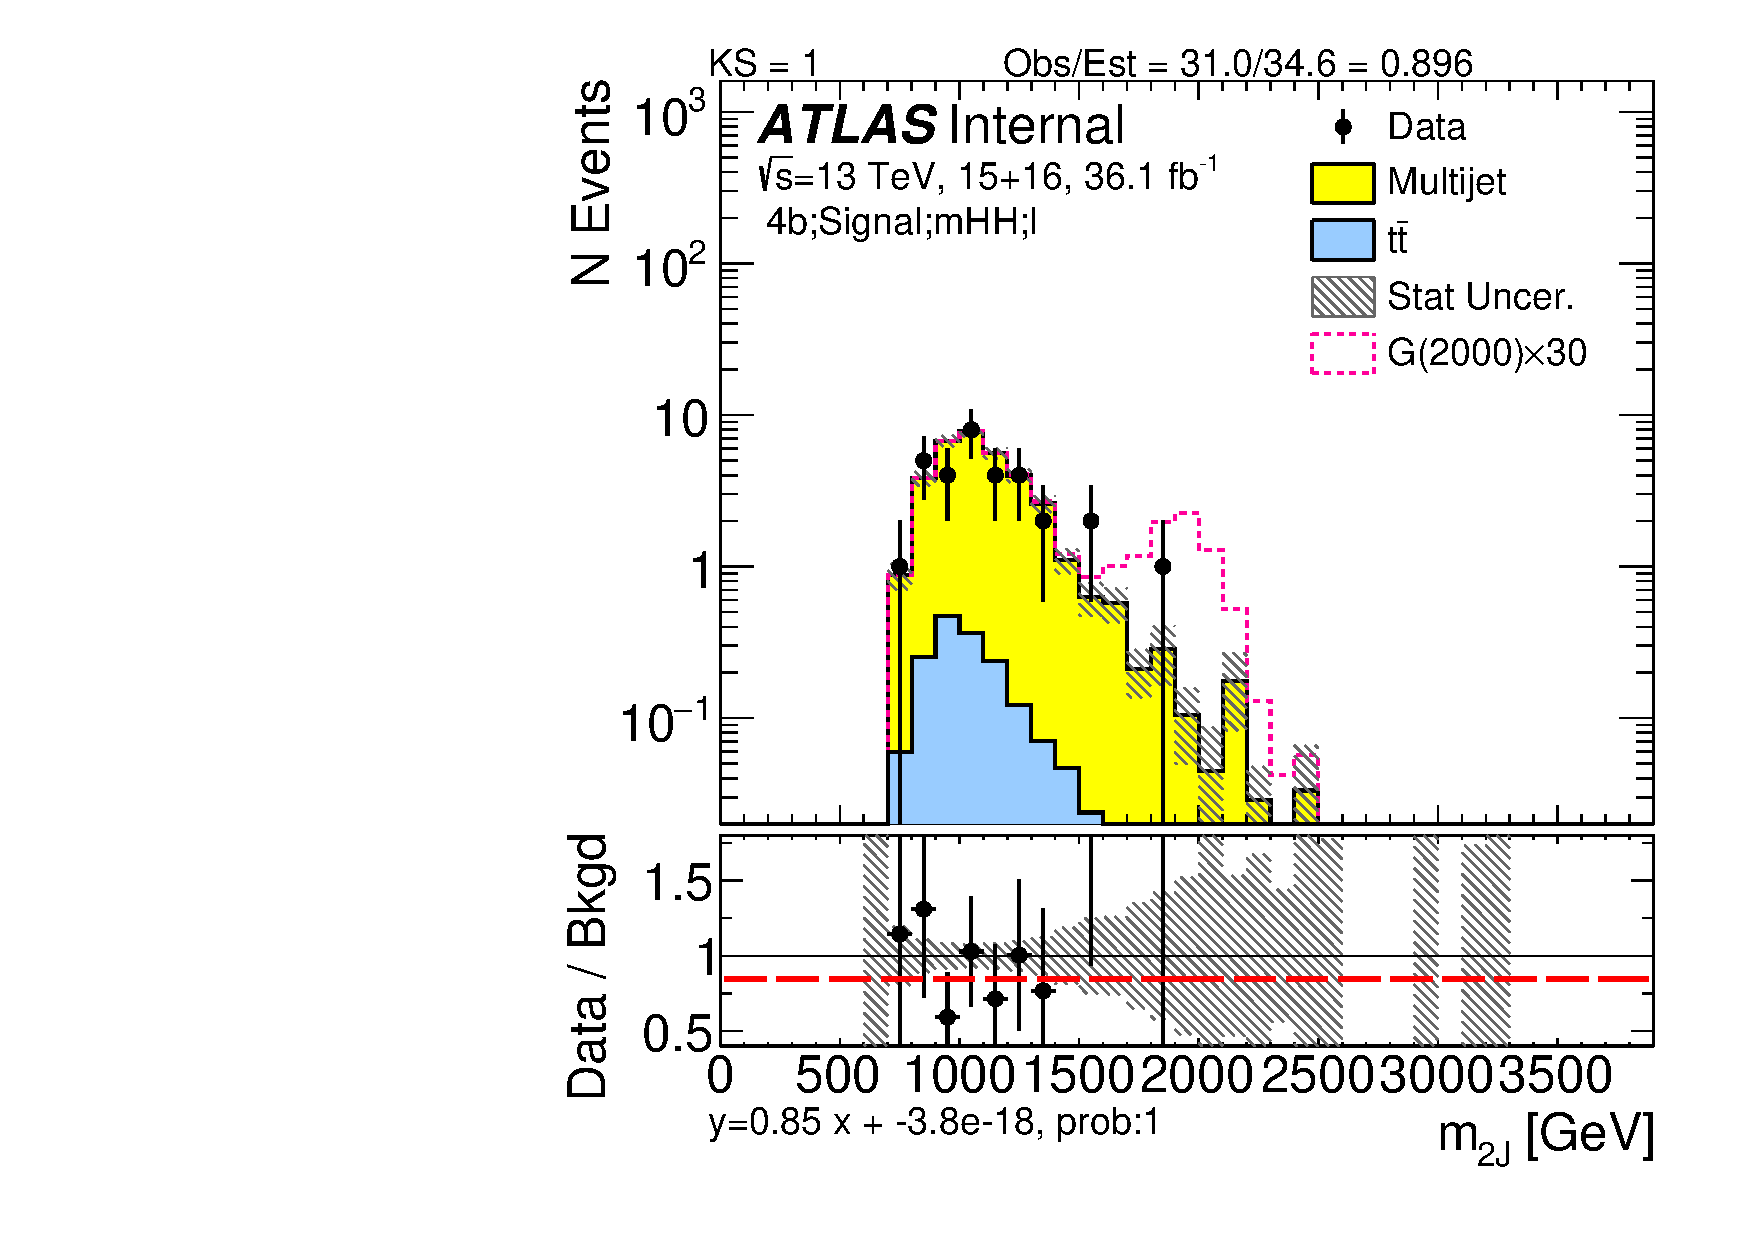
\includegraphics[angle=270, width=0.31\textwidth]{./figures/boosted/Signal_Syst/b77_FourTag_Signal_mHH_l_1.pdf}
  \caption{Unscaled dijet mass distribution in the 4$b$ Signal Region after unblinding. The left plot is on linear scale and the right plot is on log scale. Stat uncertainty and systematic ucnertainties are shown on the plot.}
  \label{fig:boosted-4b-signal-l}
\end{center}
\end{figure*}

\begin{figure*}[htbp!]
\begin{center}
%\includegraphics[angle=270, width=0.31\textwidth]{./figures/boosted/Signal_Syst/b77_ThreeTag_Signal_mHH_l.pdf}
%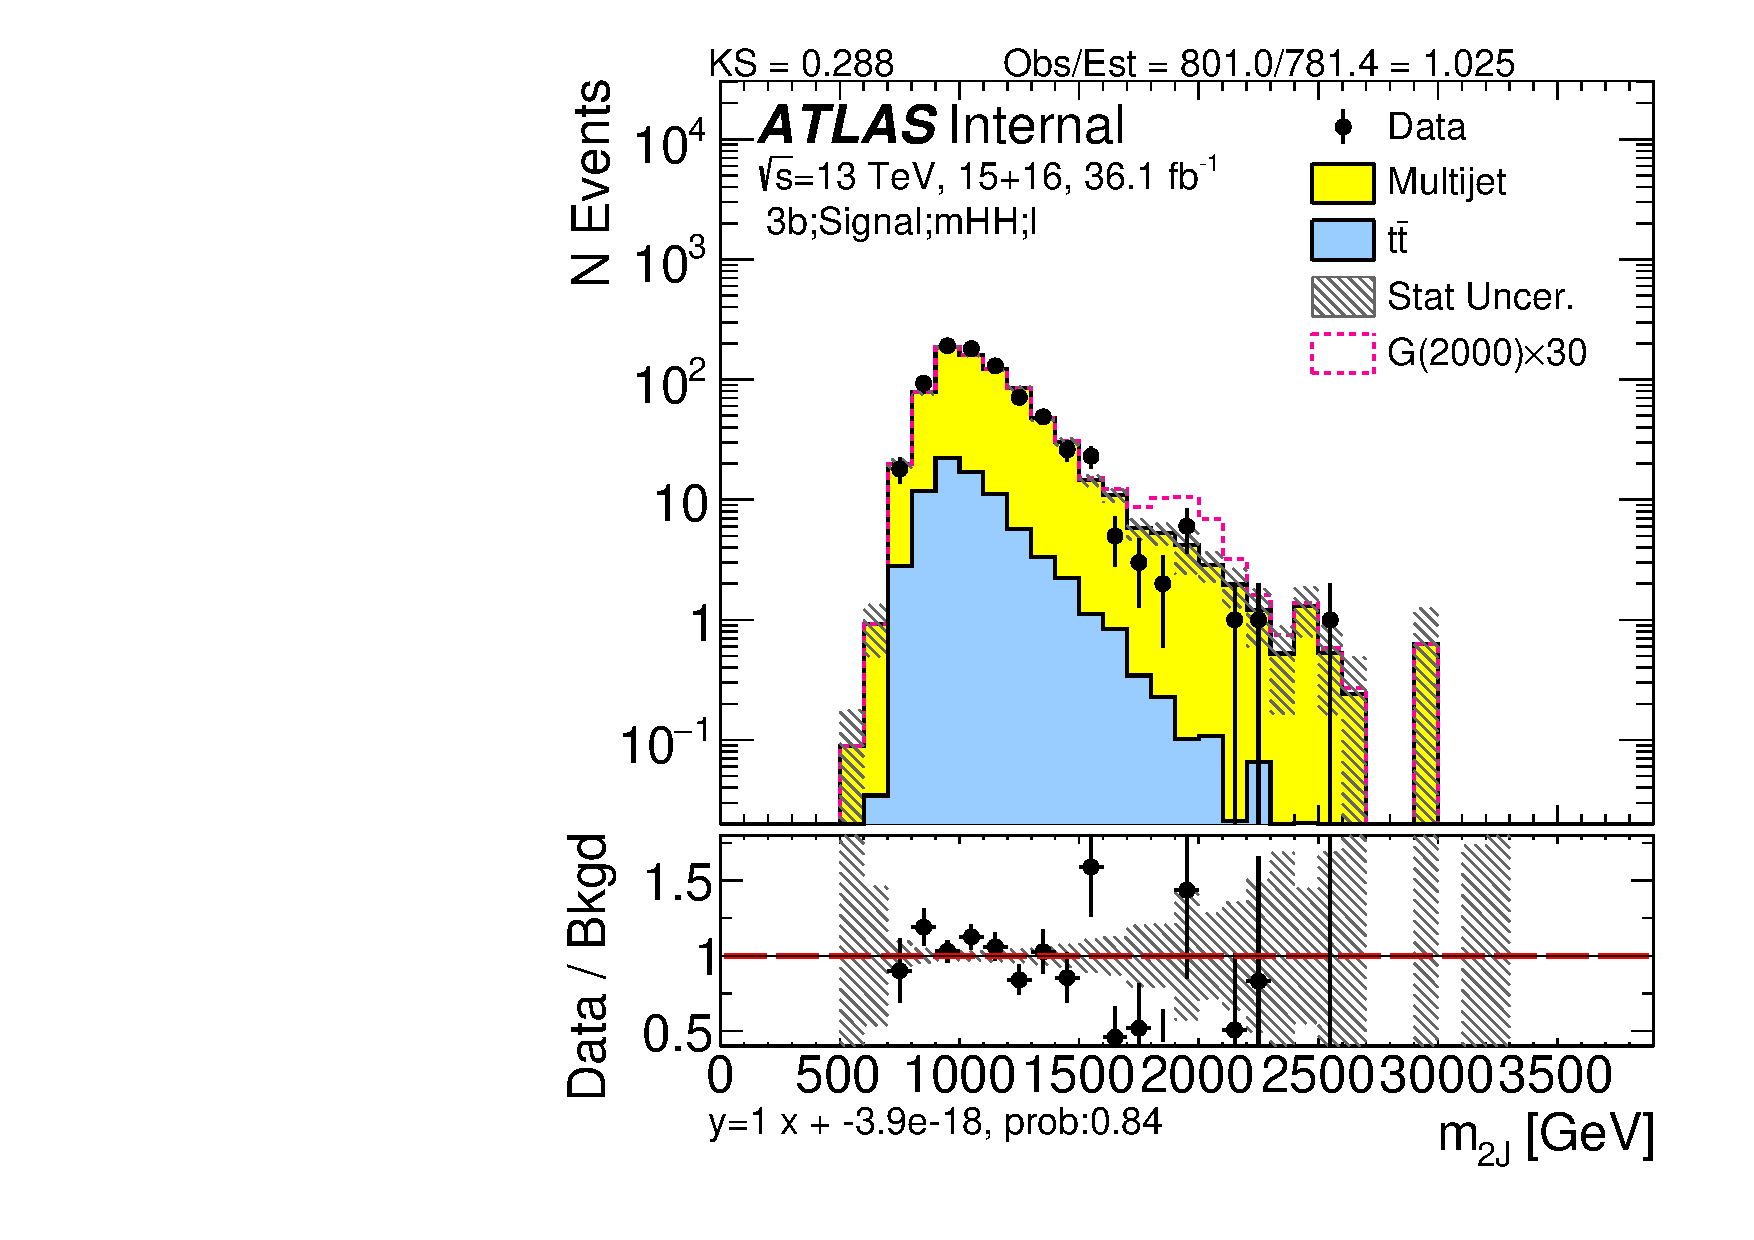
\includegraphics[angle=270, width=0.31\textwidth]{./figures/boosted/Signal_Syst/b77_ThreeTag_Signal_mHH_l_1.pdf}  
  \caption{Unscaled dijet mass distribution in the 3$b$ Signal Region after unblinding. The left plot is on linear scale and the right plot is on log scale. Stat uncertainty and systematic ucnertainties are shown on the plot.}
  \label{fig:boosted-3b-signal-l}
\end{center}
\end{figure*}

\begin{figure*}[htbp!]
\begin{center}
%\includegraphics[angle=270, width=0.31\textwidth]{./figures/boosted/Signal_Syst/b77_TwoTag_split_Signal_mHH_l.pdf}
%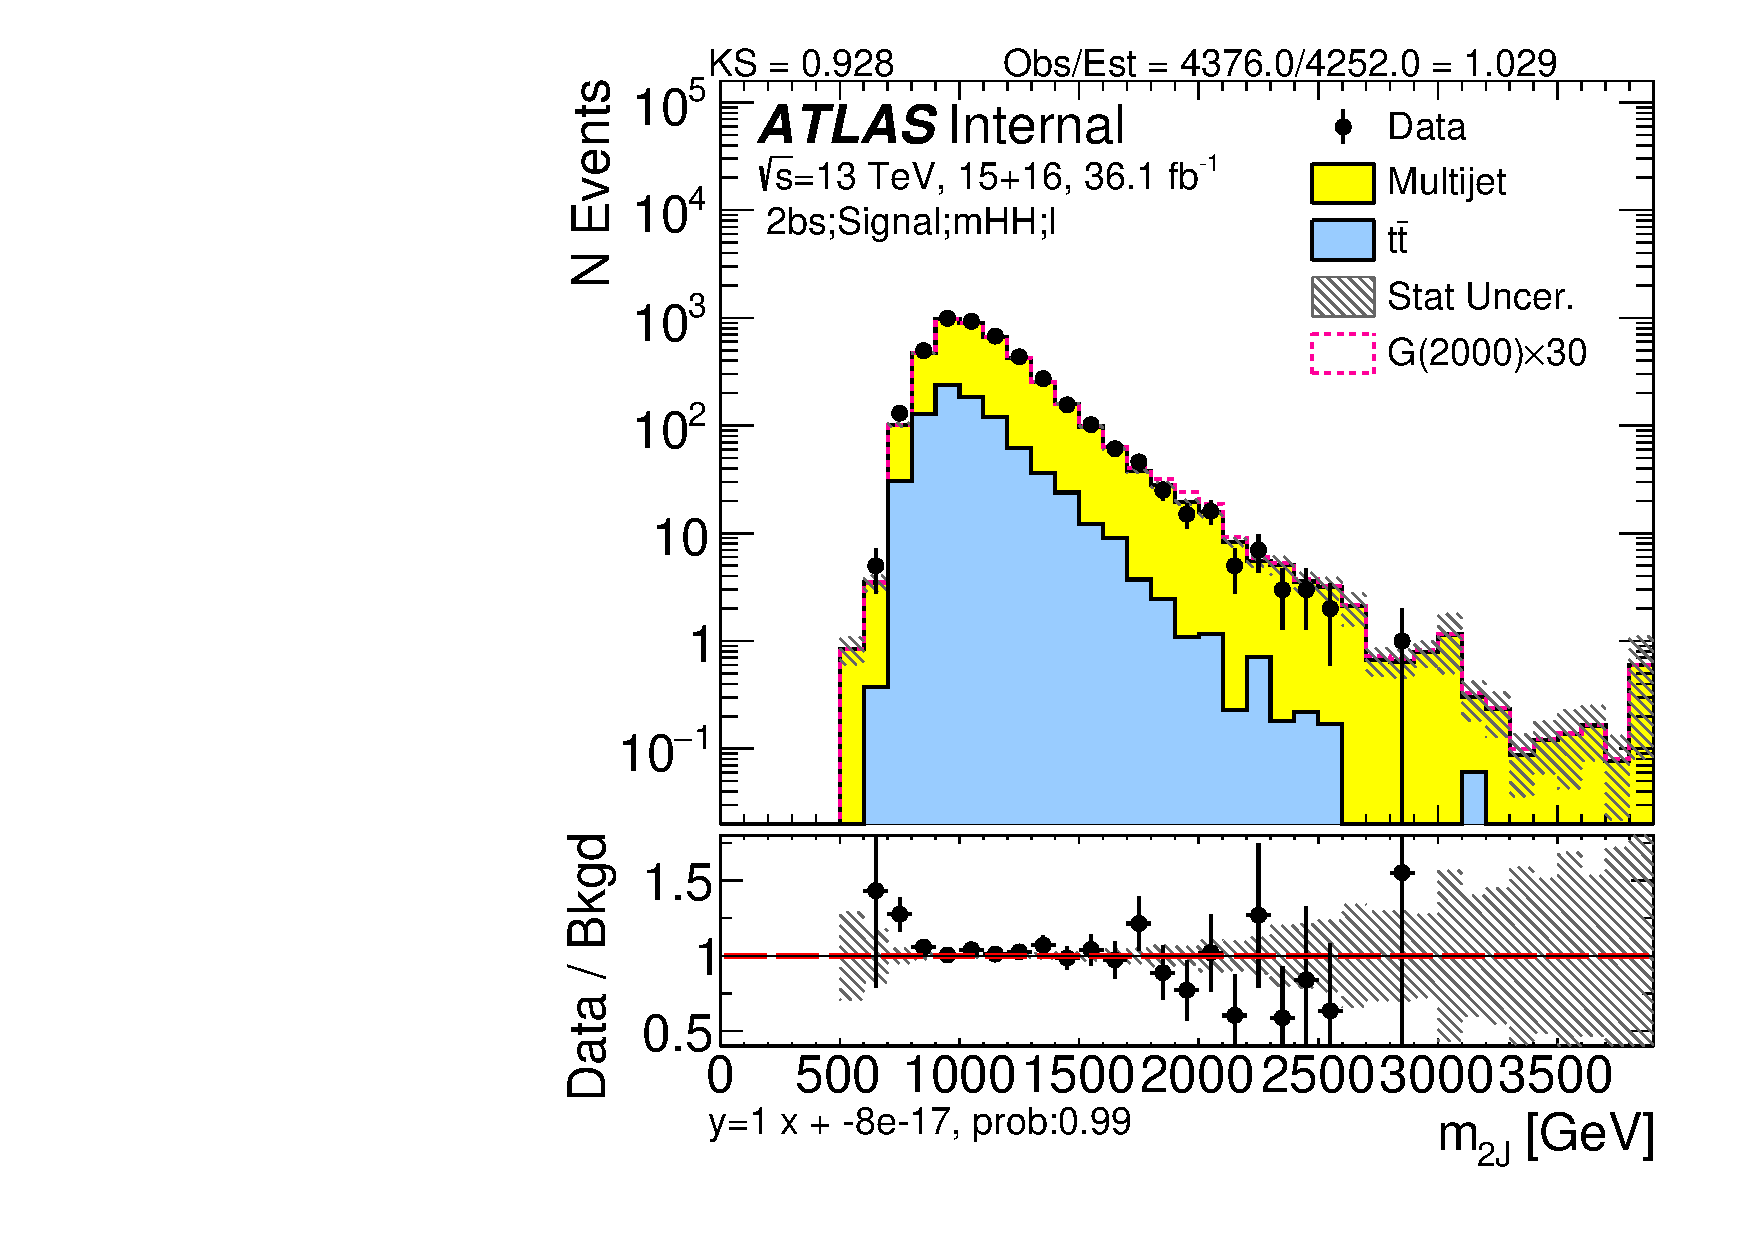
\includegraphics[angle=270, width=0.31\textwidth]{./figures/boosted/Signal_Syst/b77_TwoTag_split_Signal_mHH_l_1.pdf}  
  \caption{Unscaled dijet mass distribution in the 2$b$s Signal Region after unblinding. The left plot is on linear scale and the right plot is on log scale. Stat uncertainty and systematic ucnertainties are shown on the plot.}
  \label{fig:boosted-2b-signal-l}
\end{center}
\end{figure*}

\begin{figure*}[htbp!]
\begin{center}
%\includegraphics[angle=270, width=0.31\textwidth]{./figures/boosted/Signal_Syst/b77_FourTag_Signal_mHH_pole.pdf}
%\includegraphics[angle=270, width=0.31\textwidth]{./figures/boosted/Signal_Syst/b77_FourTag_Signal_mHH_pole_1.pdf}
  \caption{Scaled dijet mass distribution in the 4$b$ Signal Region after unblinding. The left plot is on linear scale and the right plot is on log scale. Stat uncertainty and systematic ucnertainties are shown on the plot.}
  \label{fig:boosted-4b-signal-pole}
\end{center}
\end{figure*}

\begin{figure*}[htbp!]
\begin{center}
%\includegraphics[angle=270, width=0.31\textwidth]{./figures/boosted/Signal_Syst/b77_ThreeTag_Signal_mHH_pole.pdf}
%\includegraphics[angle=270, width=0.31\textwidth]{./figures/boosted/Signal_Syst/b77_ThreeTag_Signal_mHH_pole_1.pdf}  
  \caption{Scaled dijet mass distribution in the 3$b$ Signal Region after unblinding. The left plot is on linear scale and the right plot is on log scale. Stat uncertainty and systematic ucnertainties are shown on the plot.}
  \label{fig:boosted-3b-signal-pole}
\end{center}
\end{figure*}

\begin{figure*}[htbp!]
\begin{center}
%\includegraphics[angle=270, width=0.31\textwidth]{./figures/boosted/Signal_Syst/b77_TwoTag_split_Signal_mHH_pole.pdf}
%\includegraphics[angle=270, width=0.31\textwidth]{./figures/boosted/Signal_Syst/b77_TwoTag_split_Signal_mHH_pole_1.pdf}  
  \caption{Scaled dijet mass distribution in the 2$b$s Signal Region after unblinding. The left plot is on linear scale and the right plot is on log scale. Stat uncertainty and systematic ucnertainties are shown on the plot.}
  \label{fig:boosted-2b-signal-pole}
\end{center}
\end{figure*}

\clearpage
\subsection{Kinematic Distributions}
This section shows unblinded comparisons of data with the prediction of QCD multi-jets and \ttbar in the signal region (SR). Plots shown are with stat uncertainty only.

Figures~\ref{fig:boosted-4b-signal-ak10-lead}, \ref{fig:boosted-4b-signal-ak10-subl}, \ref{fig:boosted-4b-signal-ak2}, and \ref{fig:boosted-4b-signal-ak10-system} show predictions of various kinematics of the large-$R$ jets and their associated track jets in the 4$b$ selection.

Figures~\ref{fig:boosted-3b-signal-ak10-lead}, \ref{fig:boosted-3b-signal-ak10-subl}, \ref{fig:boosted-3b-signal-ak2}, and \ref{fig:boosted-3b-signal-ak10-system} show predictions of various kinematics of the large-$R$ jets and their associated track jets in the 3$b$ selection.

Figures~\ref{fig:boosted-2bs-signal-ak10-lead}, \ref{fig:boosted-2bs-signal-ak10-subl}, \ref{fig:boosted-2bs-signal-ak2}, and \ref{fig:boosted-2bs-signal-ak10-system} show predictions of various kinematics of the large-$R$ jets and their associated track jets in the 2$b$ selection.

\begin{figure*}[htbp!]
\begin{center}
%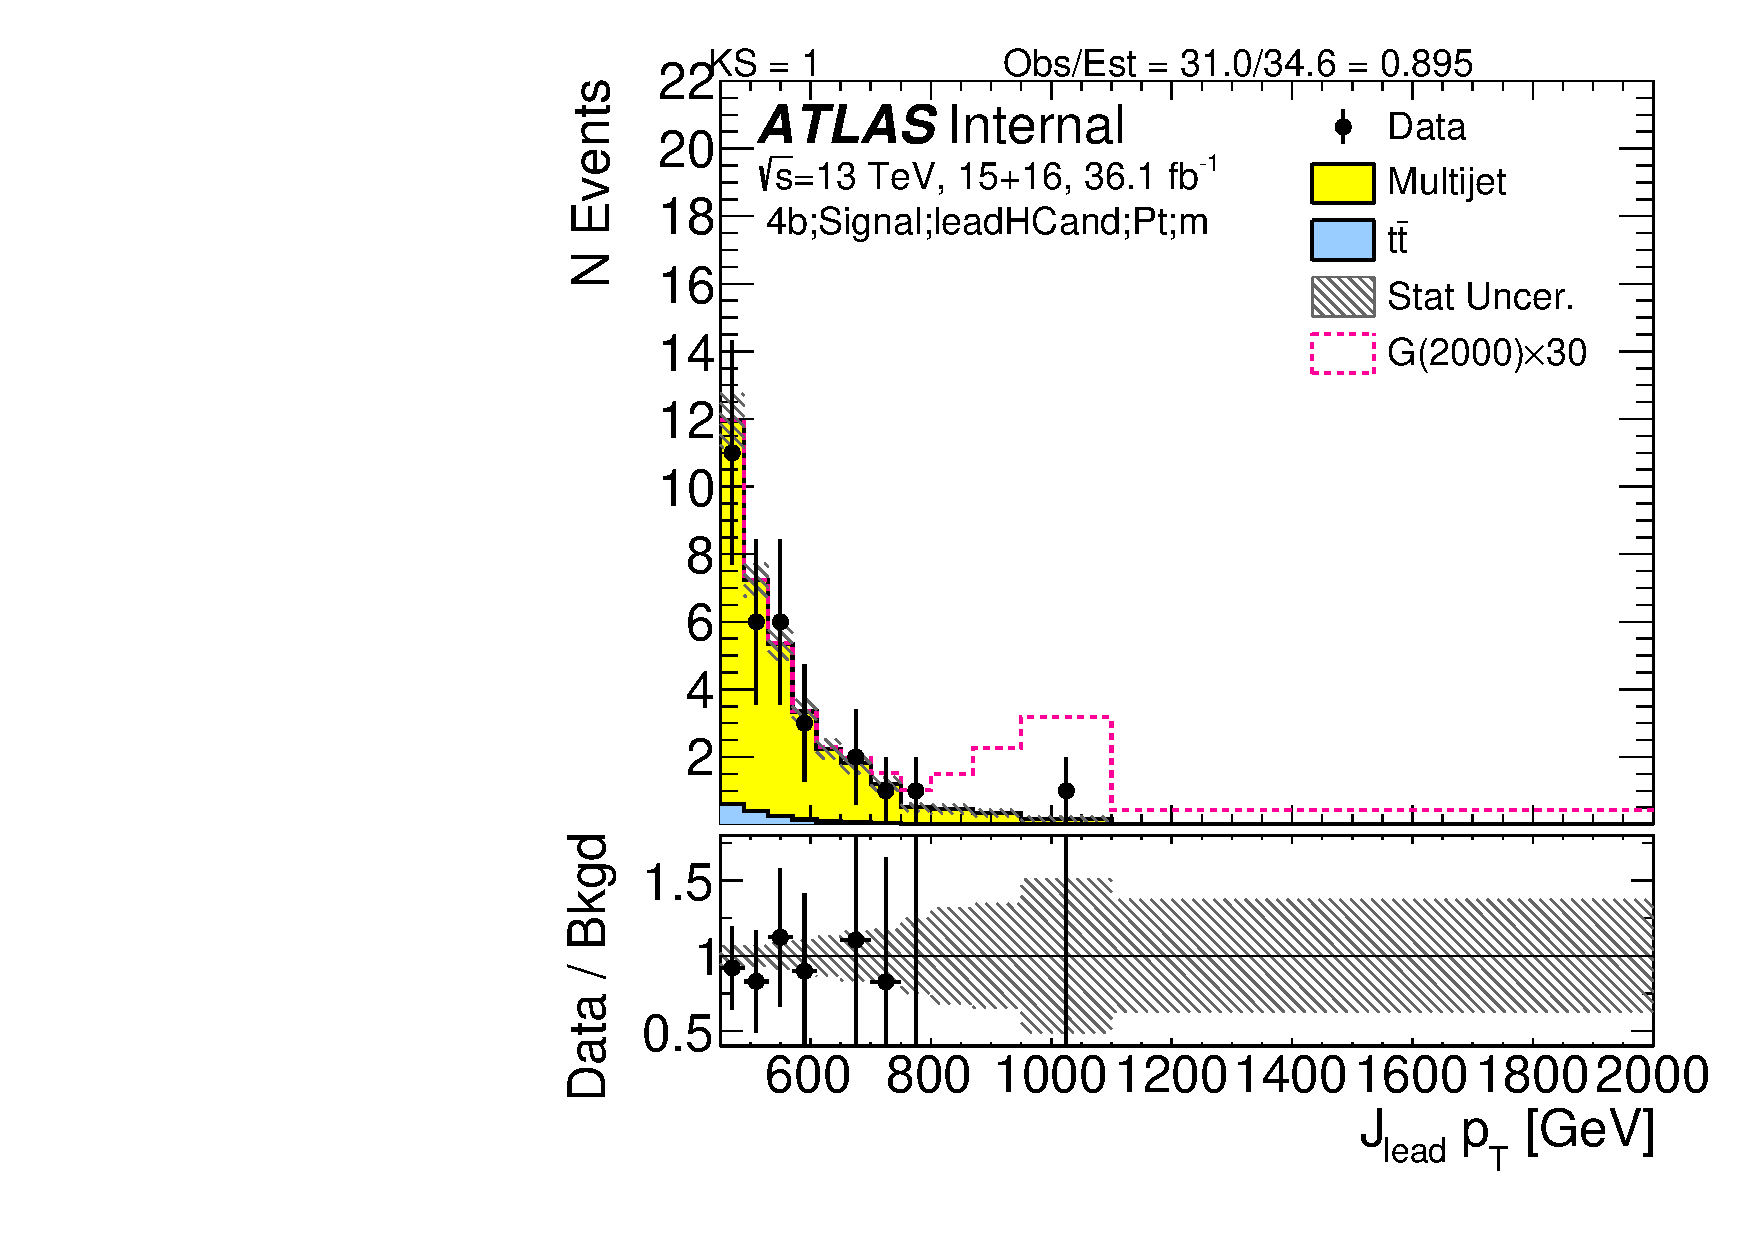
\includegraphics[angle=270, width=0.31\textwidth]{./figures/boosted/Signal/b77_FourTag_Signal_leadHCand_Pt_m.pdf}
%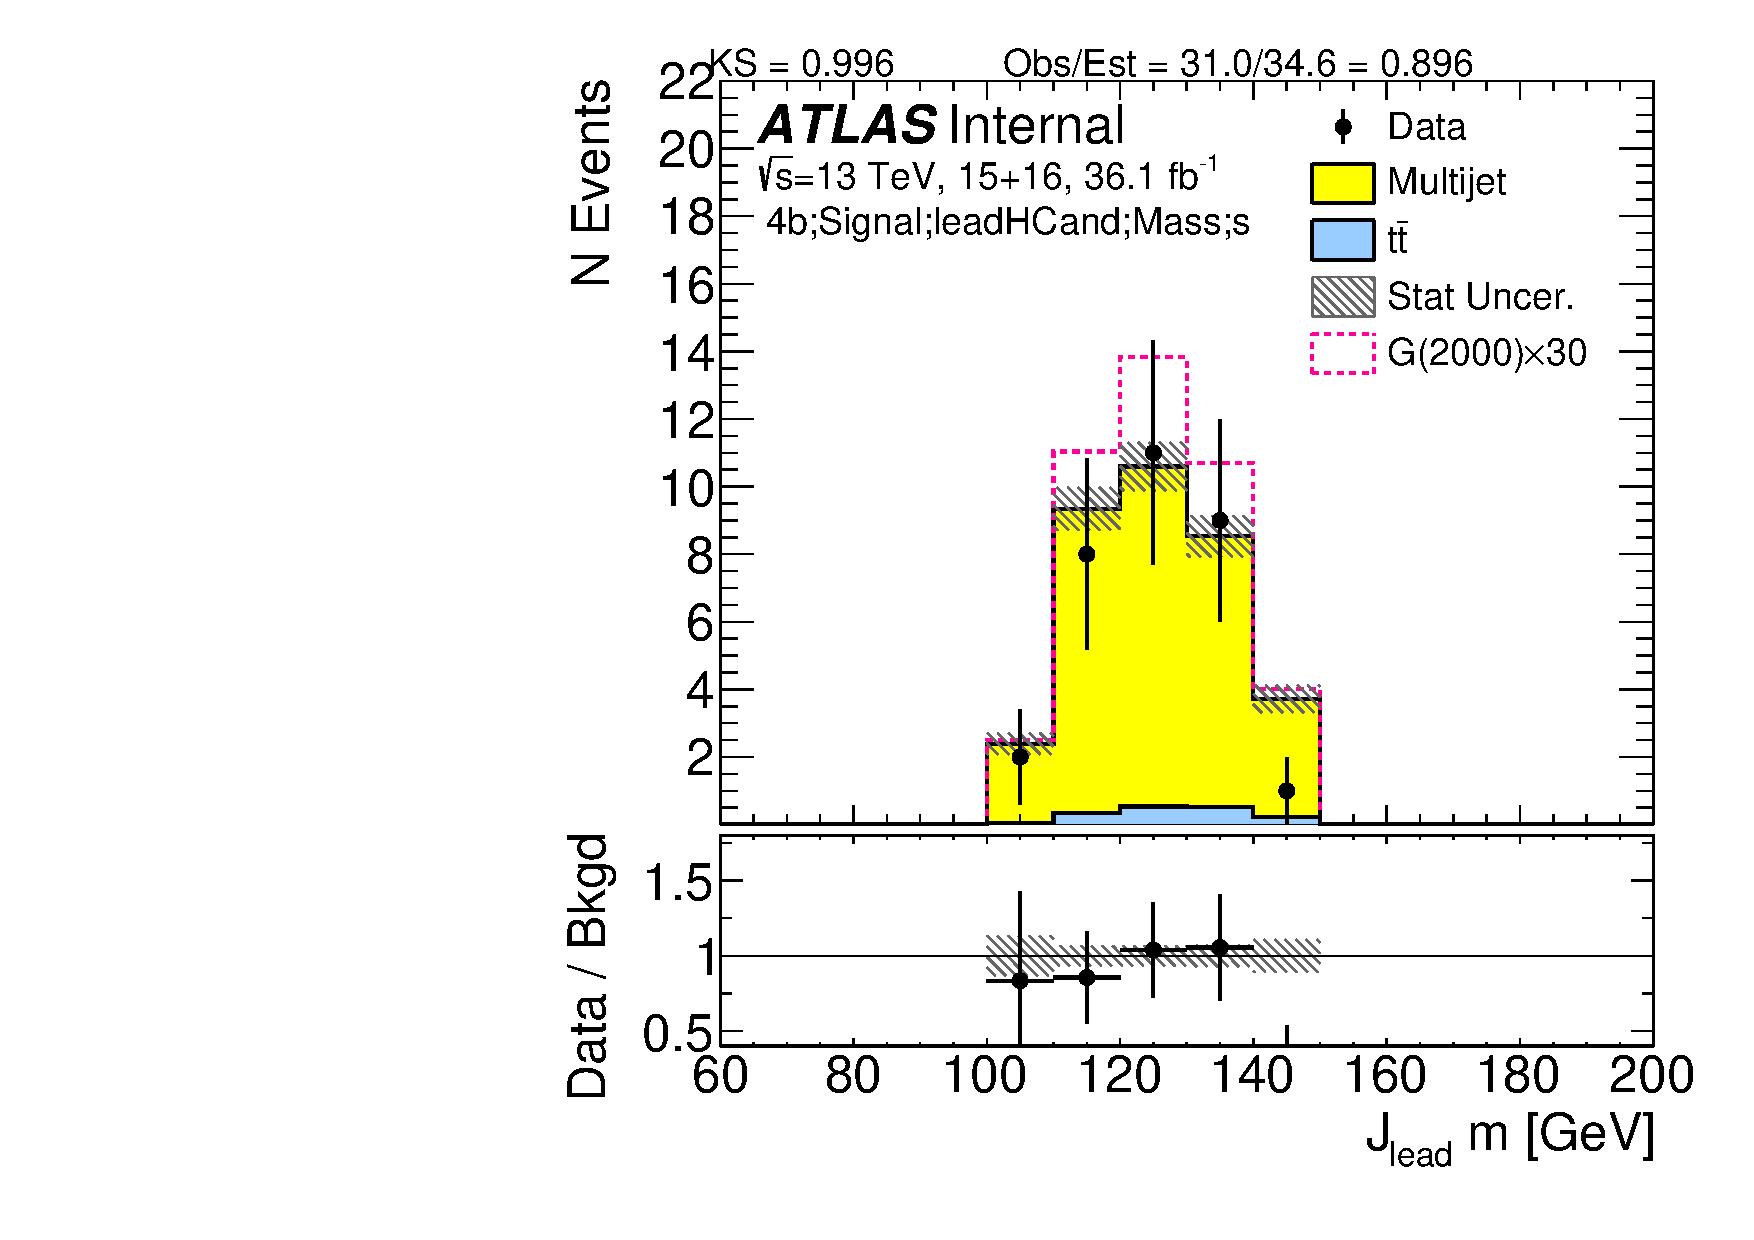
\includegraphics[angle=270, width=0.31\textwidth]{./figures/boosted/Signal/b77_FourTag_Signal_leadHCand_Mass_s.pdf}\\
%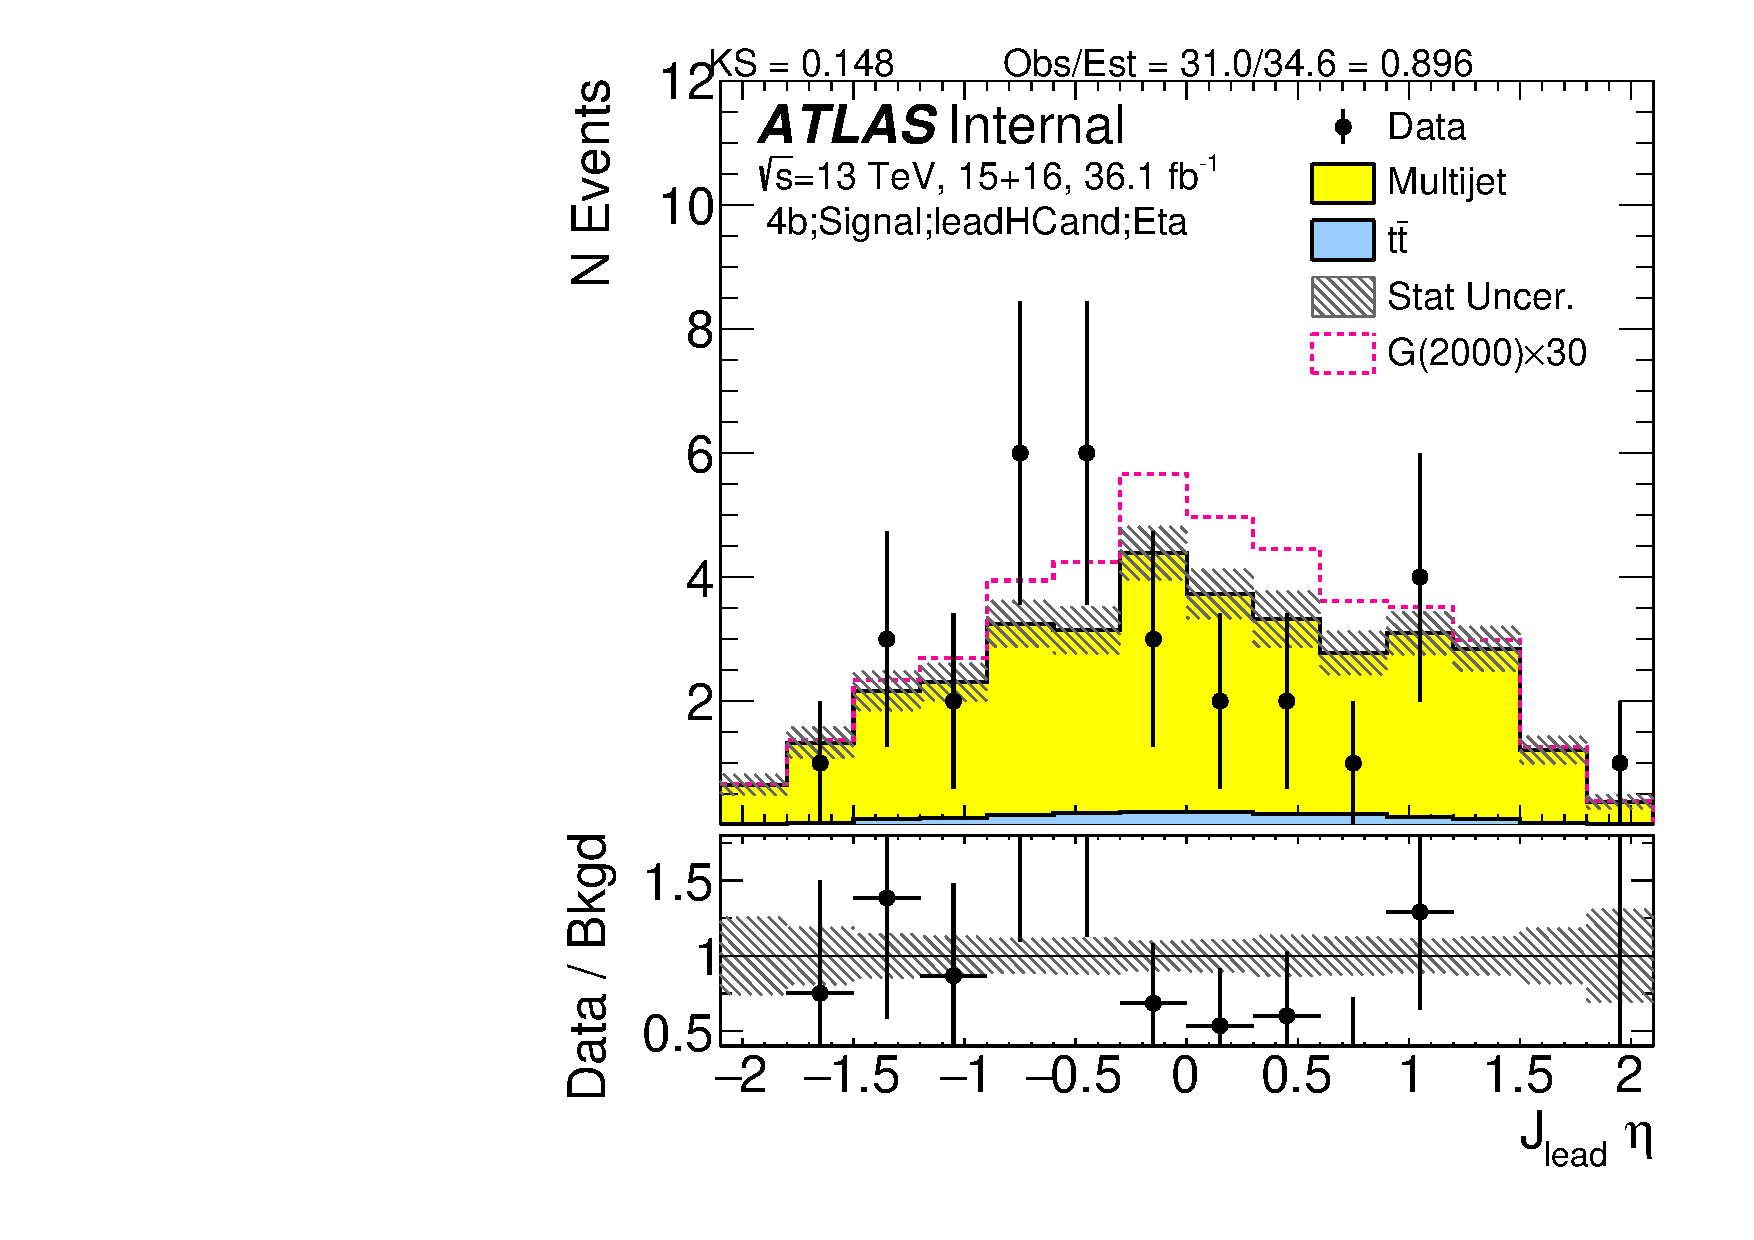
\includegraphics[angle=270, width=0.31\textwidth]{./figures/boosted/Signal/b77_FourTag_Signal_leadHCand_Eta.pdf}
%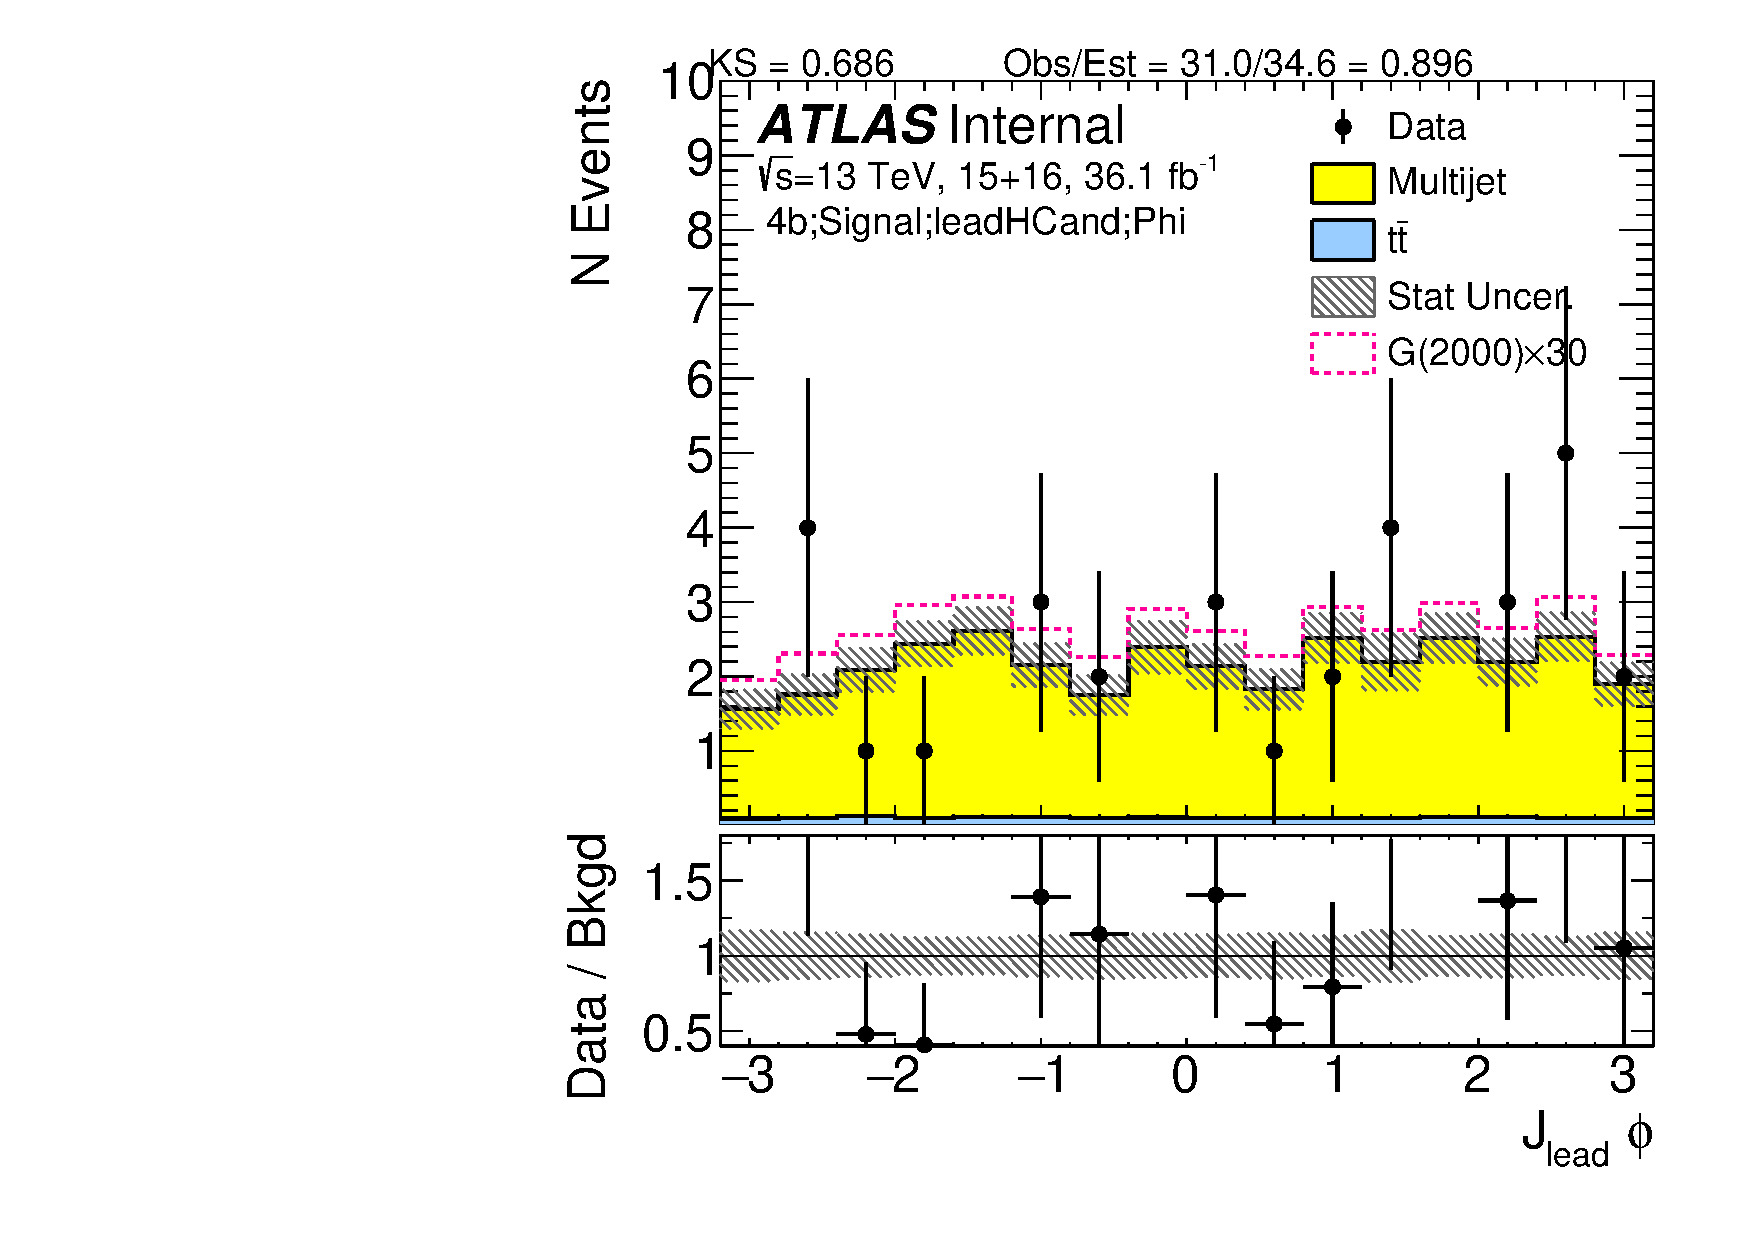
\includegraphics[angle=270, width=0.31\textwidth]{./figures/boosted/Signal/b77_FourTag_Signal_leadHCand_Phi.pdf}
  \caption{Kinematics of the lead large-$R$ jet in data and prediction in the signal region after requiring 4 $b$-tags. }
  \label{fig:boosted-4b-signal-ak10-lead}
\end{center}
\end{figure*}

\begin{figure*}[htbp!]
\begin{center}
%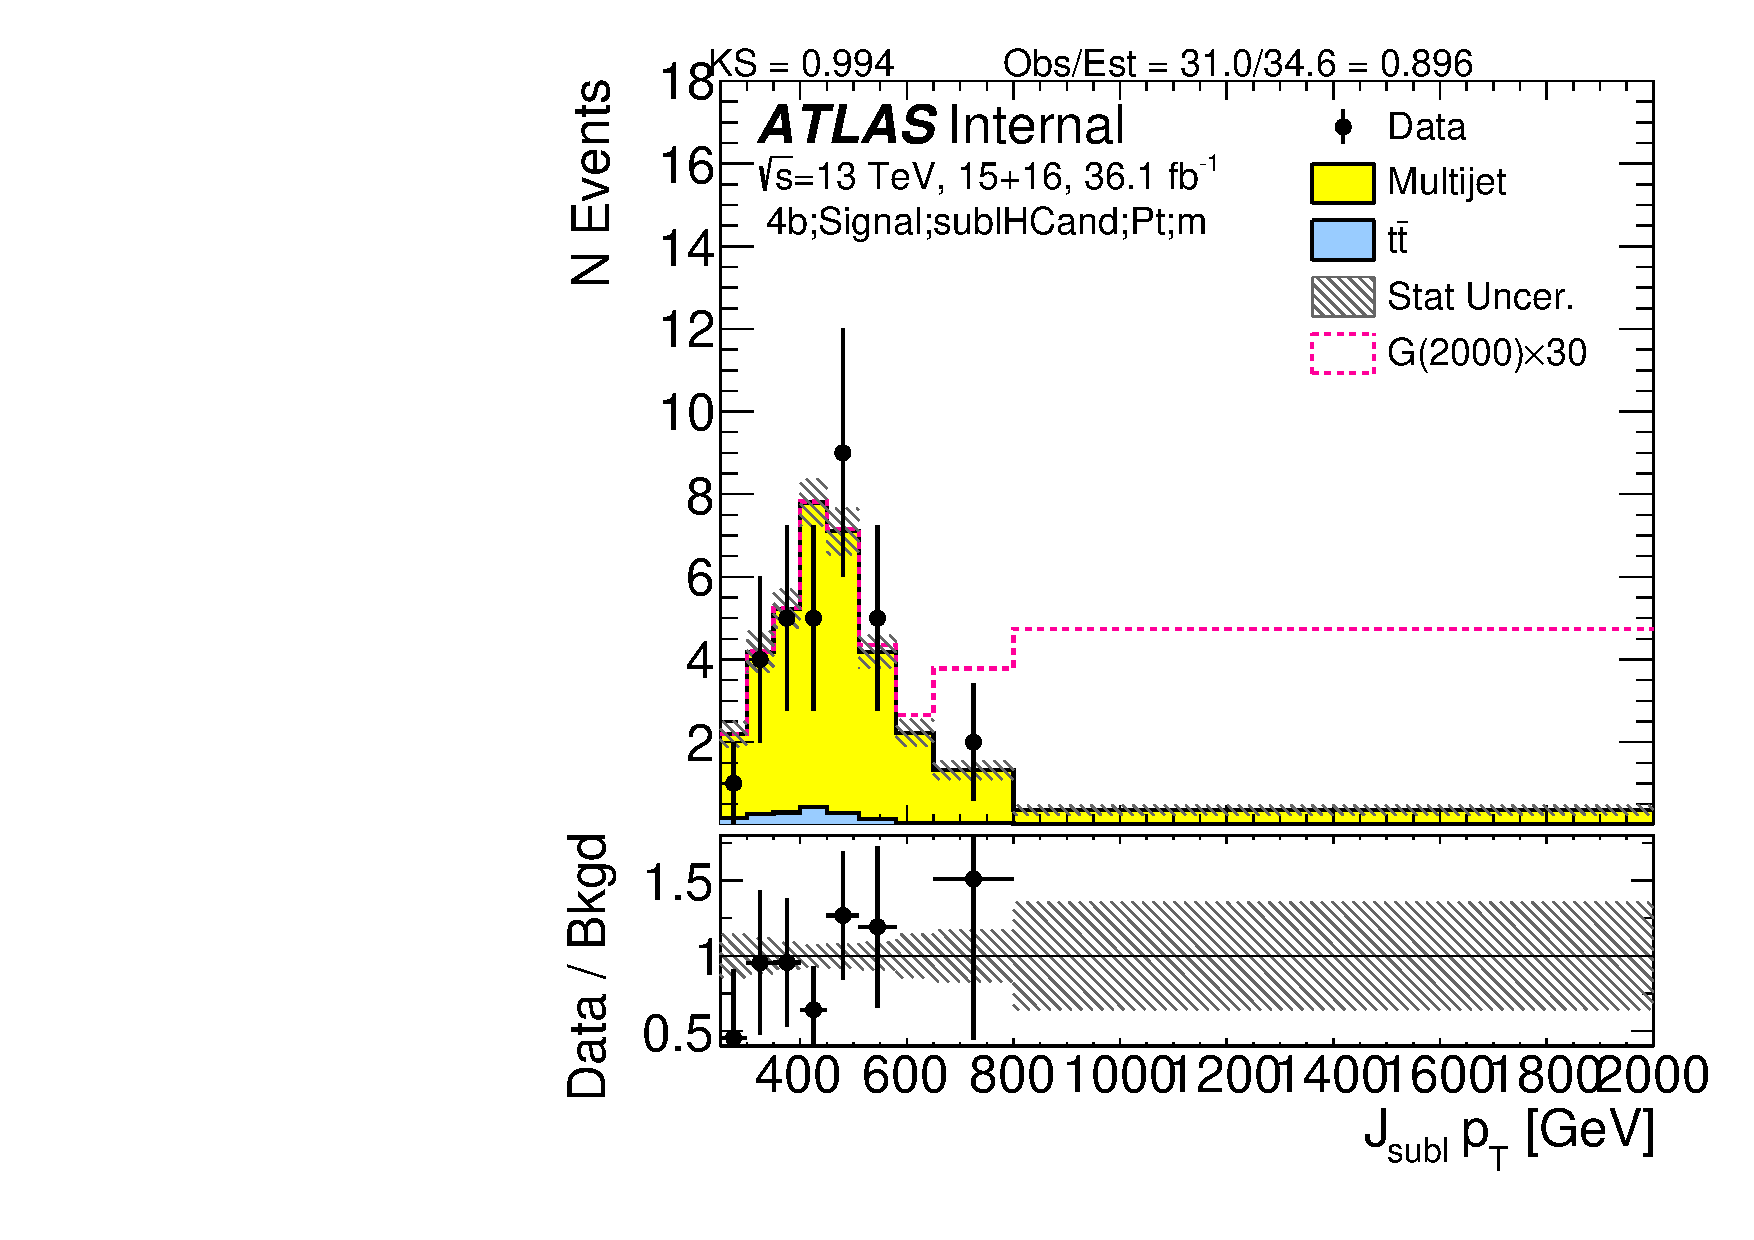
\includegraphics[angle=270, width=0.31\textwidth]{./figures/boosted/Signal/b77_FourTag_Signal_sublHCand_Pt_m.pdf}
%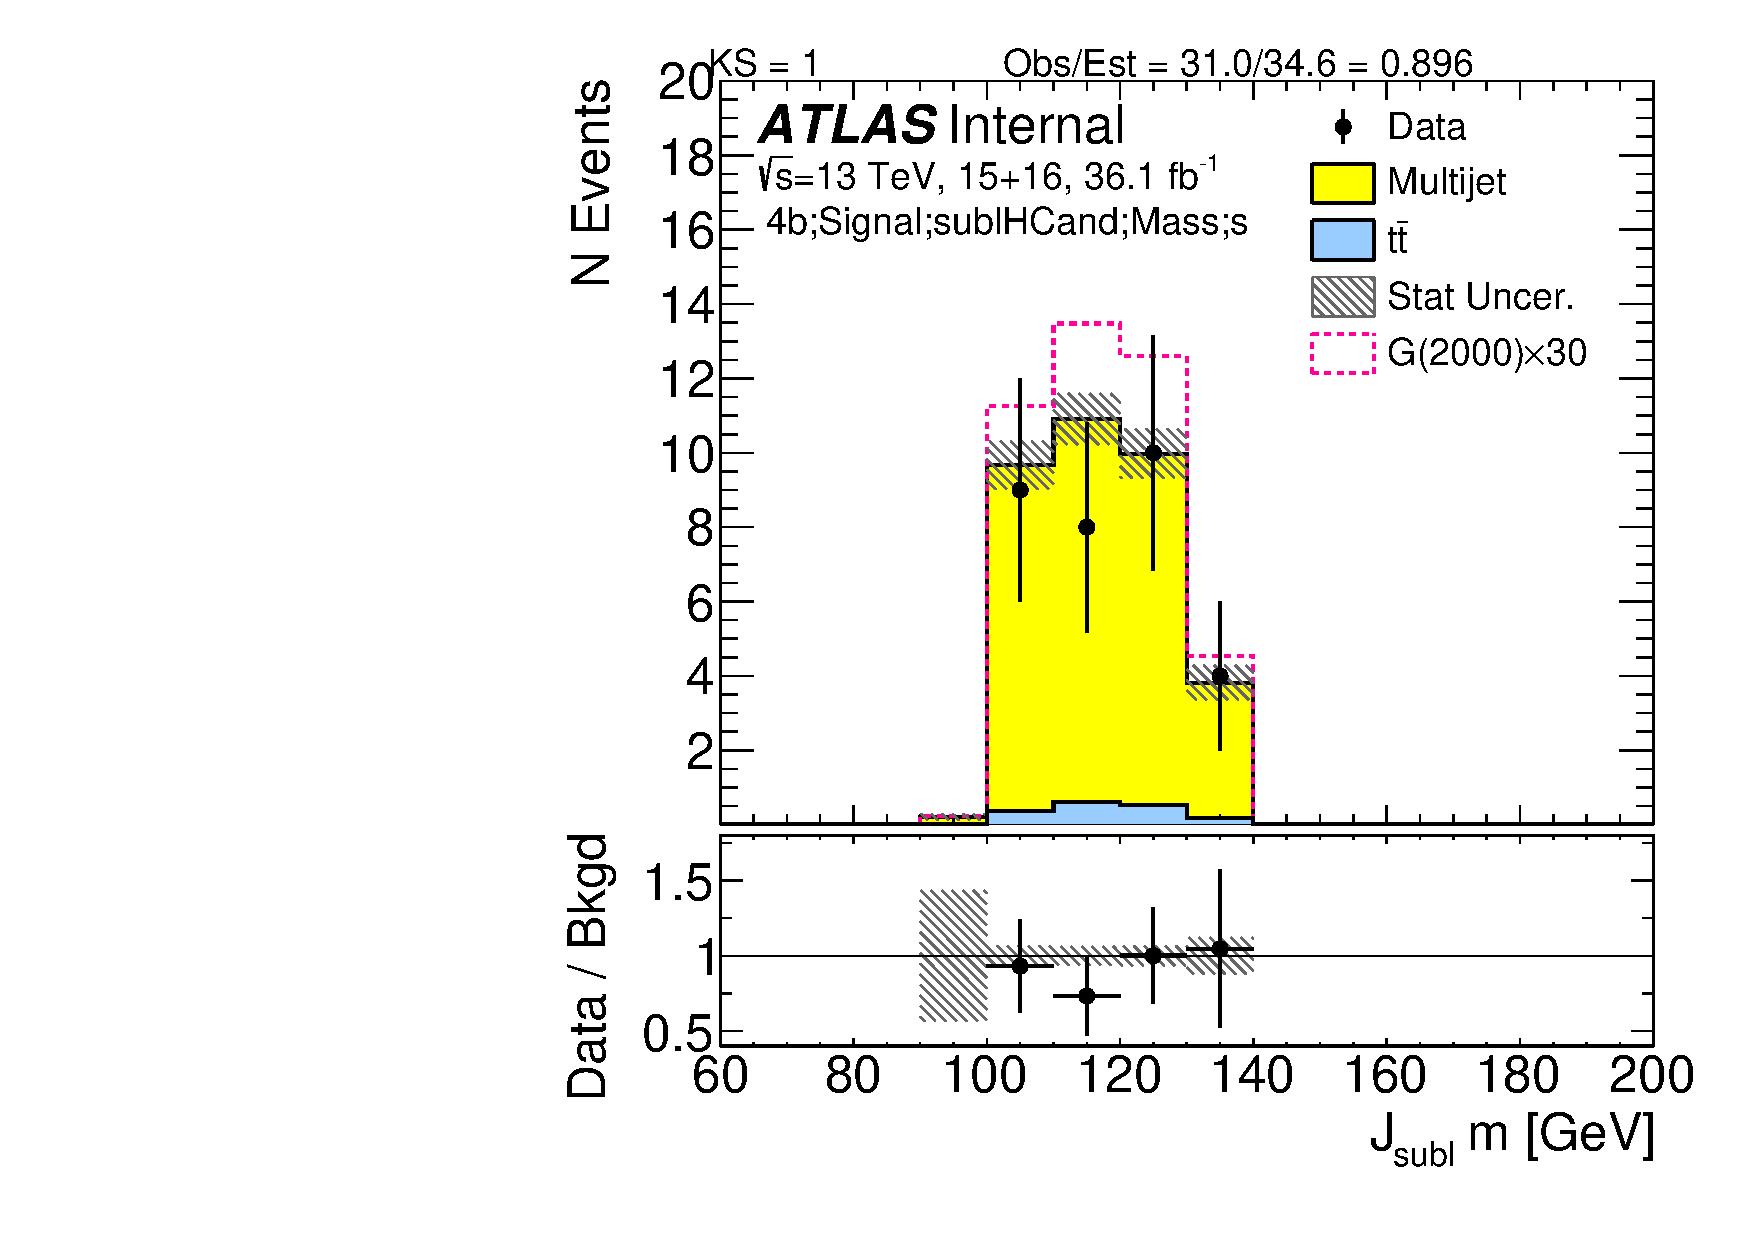
\includegraphics[angle=270, width=0.31\textwidth]{./figures/boosted/Signal/b77_FourTag_Signal_sublHCand_Mass_s.pdf}\\
%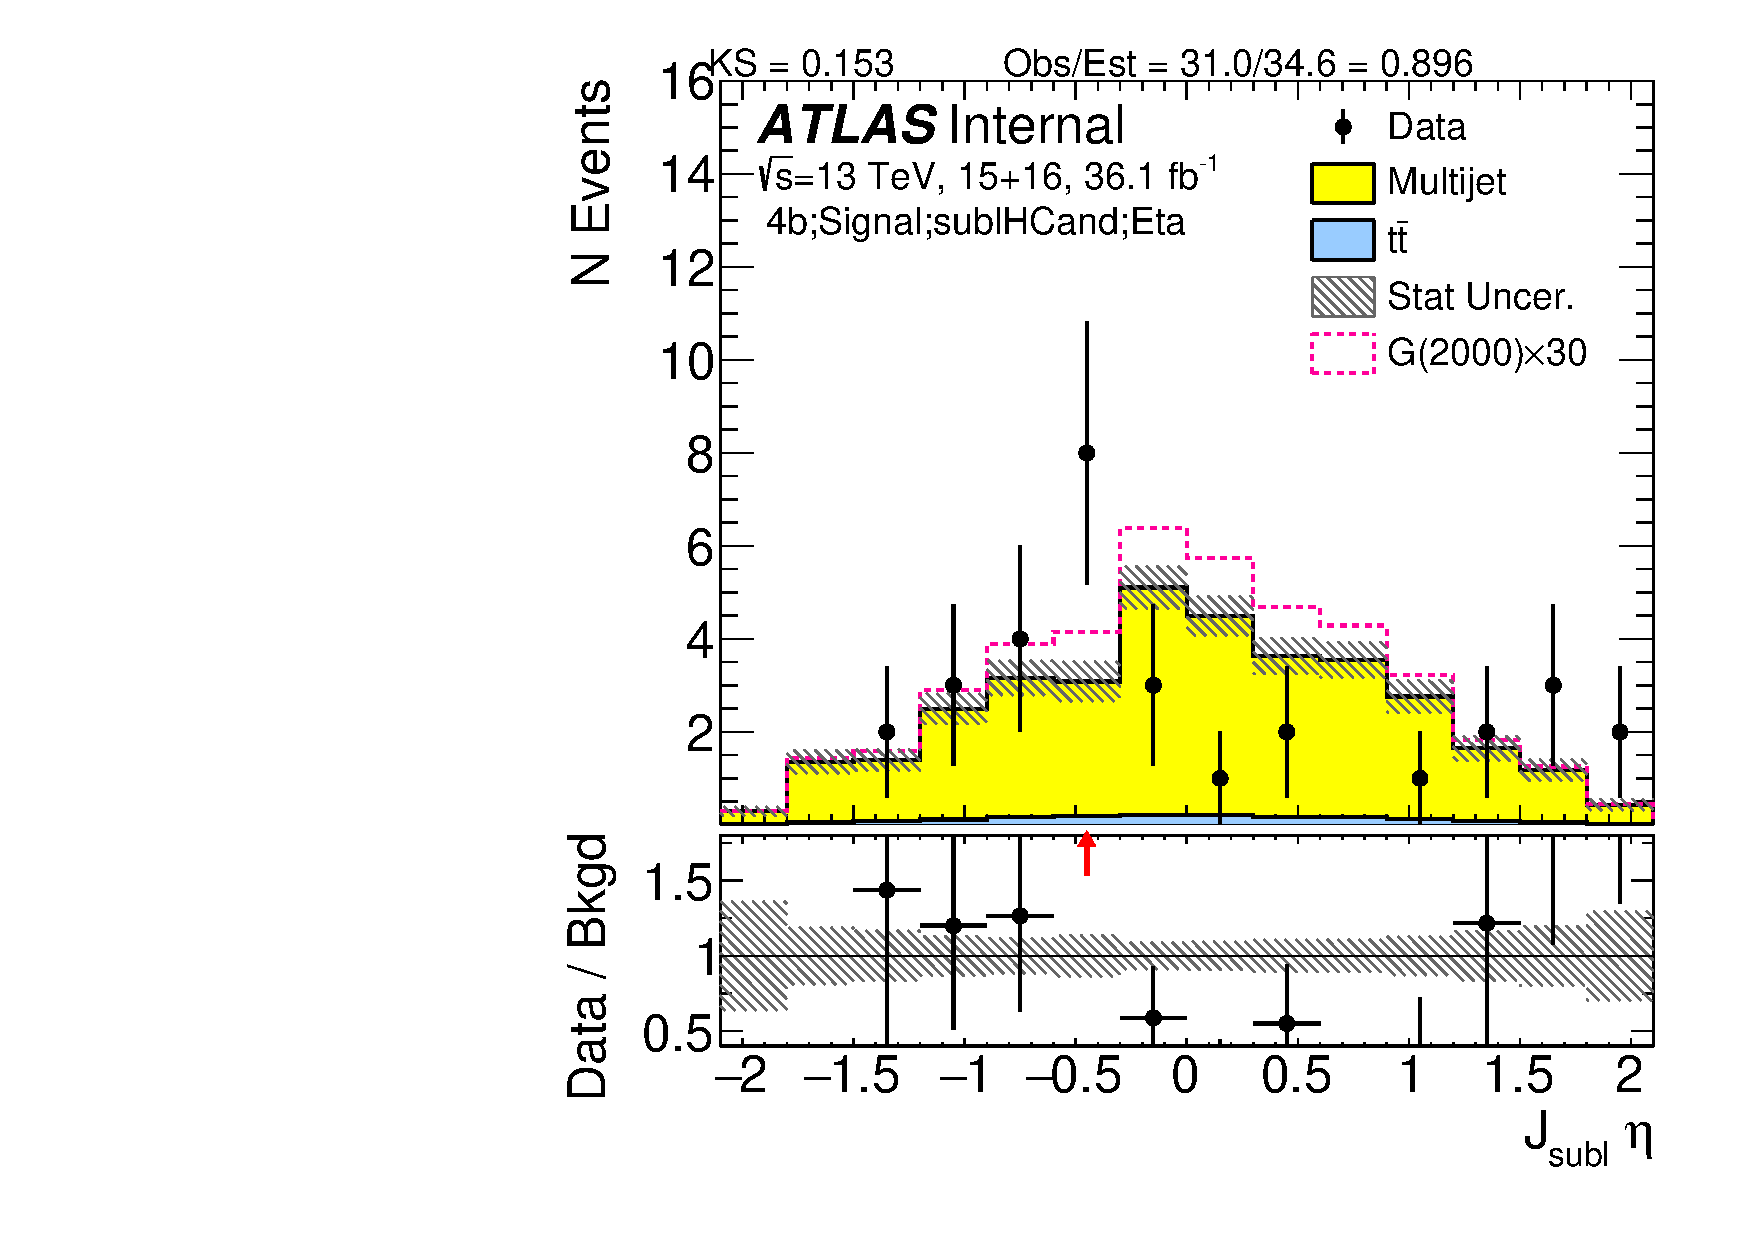
\includegraphics[angle=270, width=0.31\textwidth]{./figures/boosted/Signal/b77_FourTag_Signal_sublHCand_Eta.pdf}
%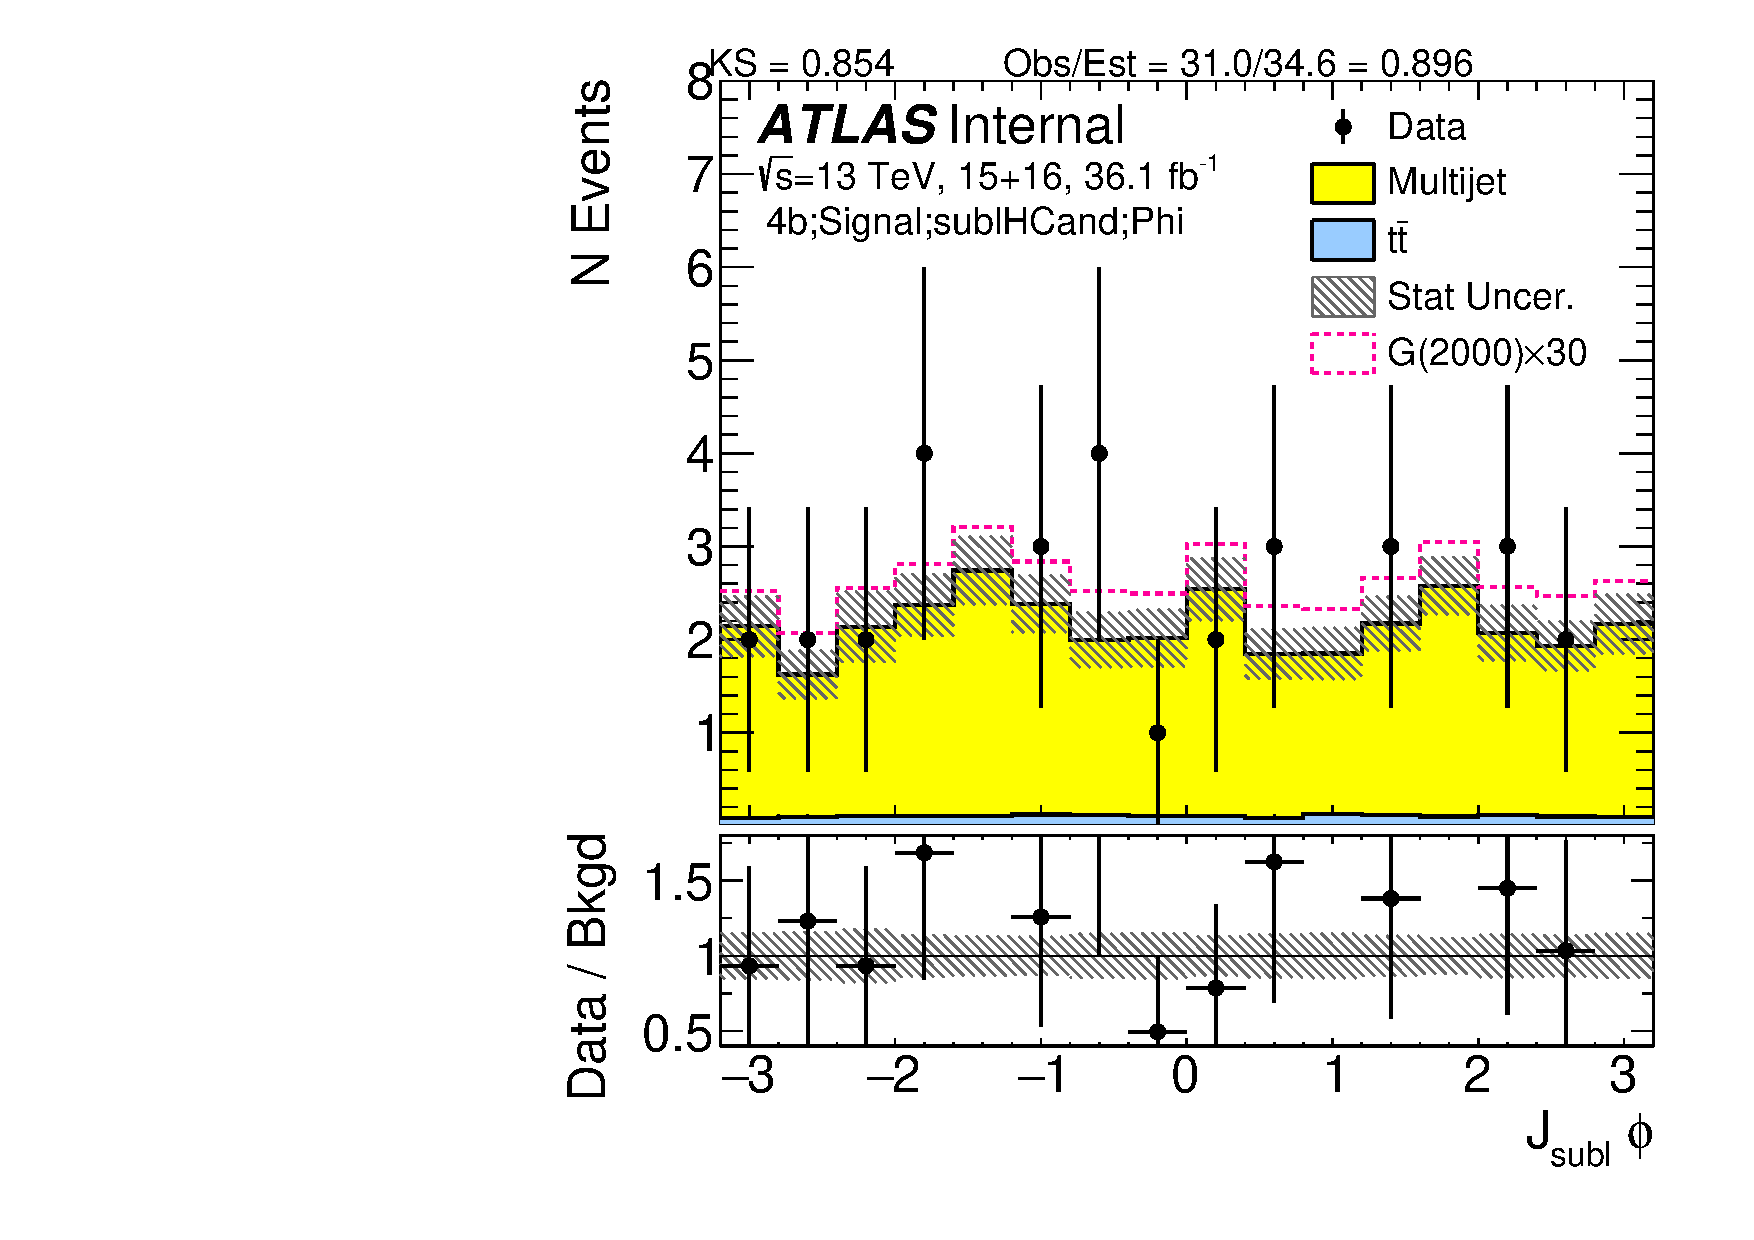
\includegraphics[angle=270, width=0.31\textwidth]{./figures/boosted/Signal/b77_FourTag_Signal_sublHCand_Phi.pdf}
  \caption{Kinematics of the sub-lead large-$R$ jet in data and prediction in the signal region after requiring 4 $b$-tags. }
  \label{fig:boosted-4b-signal-ak10-subl}
\end{center}
\end{figure*}

\begin{figure*}[htbp!]
\begin{center}
%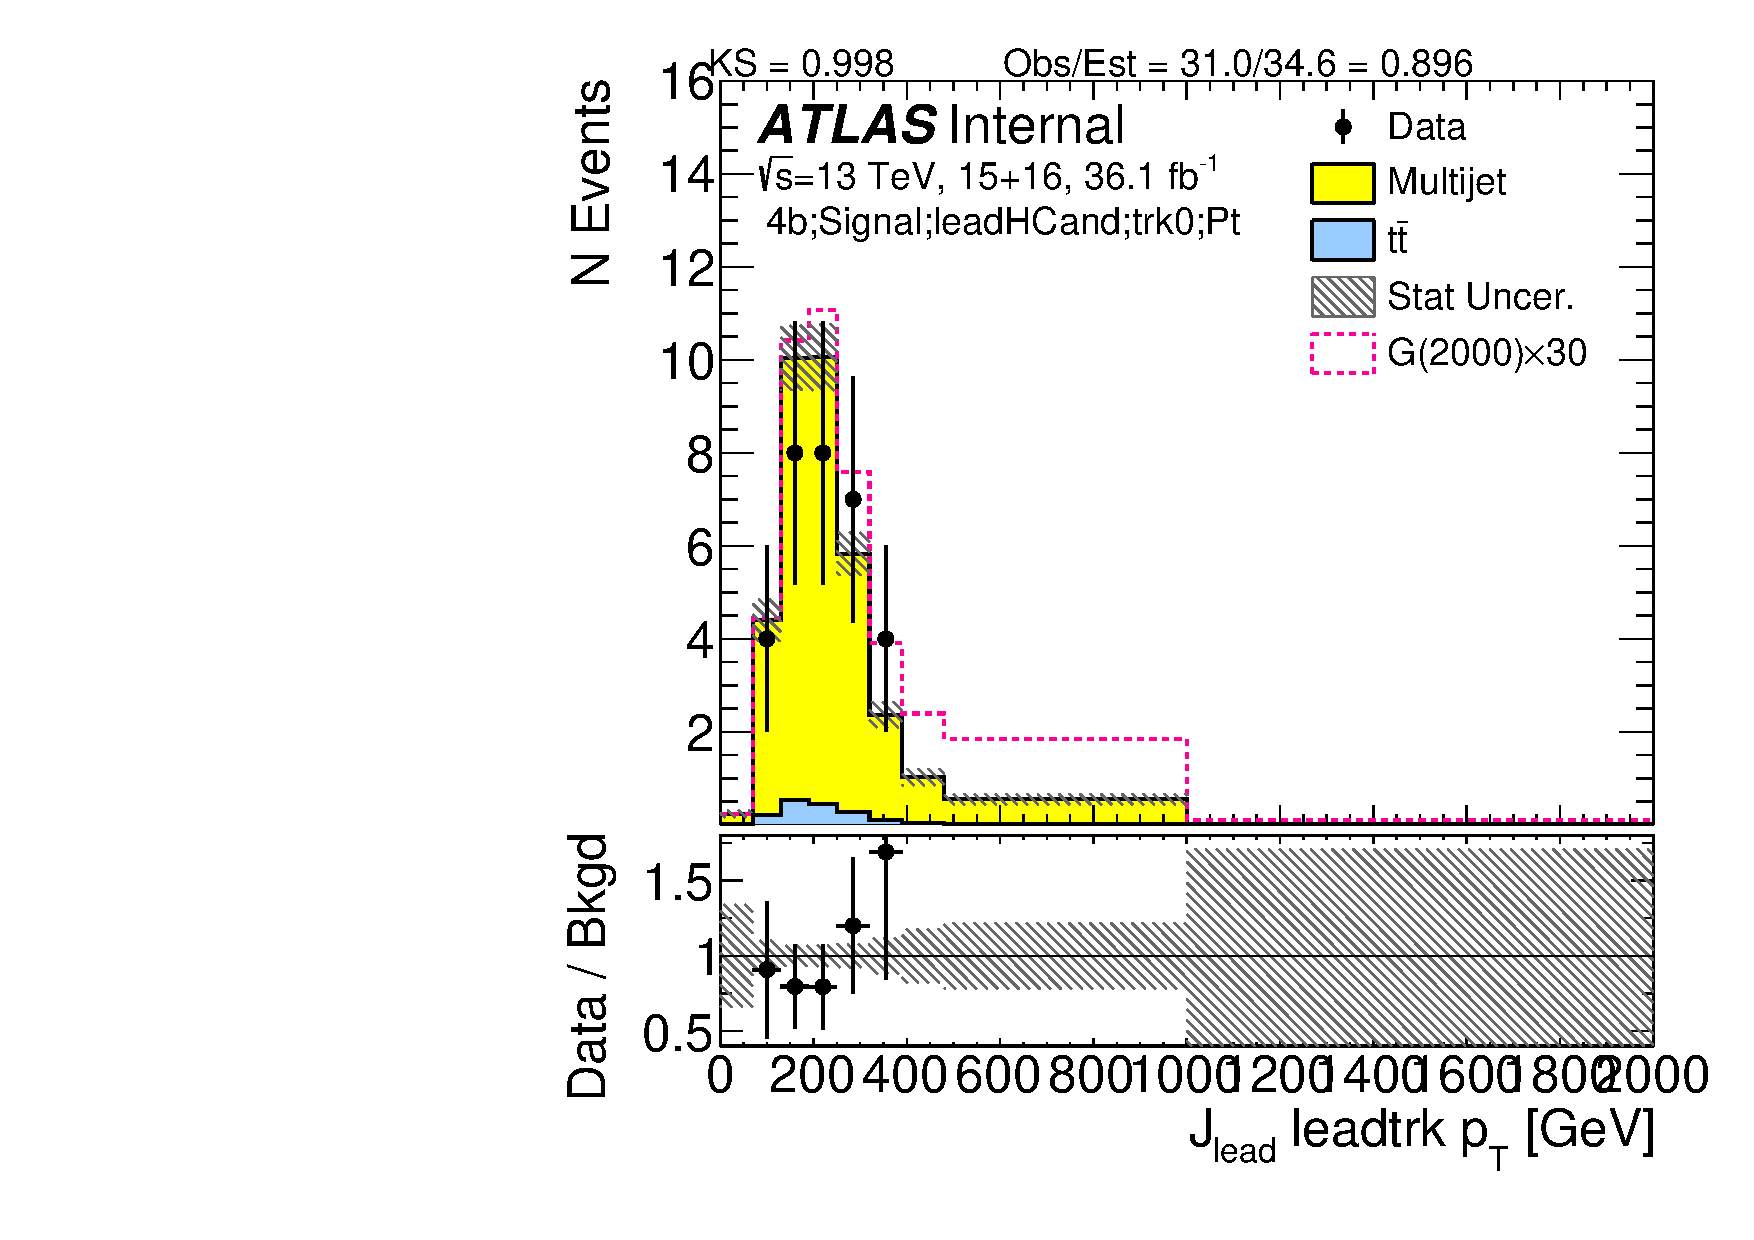
\includegraphics[angle=270, width=0.31\textwidth]{./figures/boosted/Signal/b77_FourTag_Signal_leadHCand_trk0_Pt.pdf}
%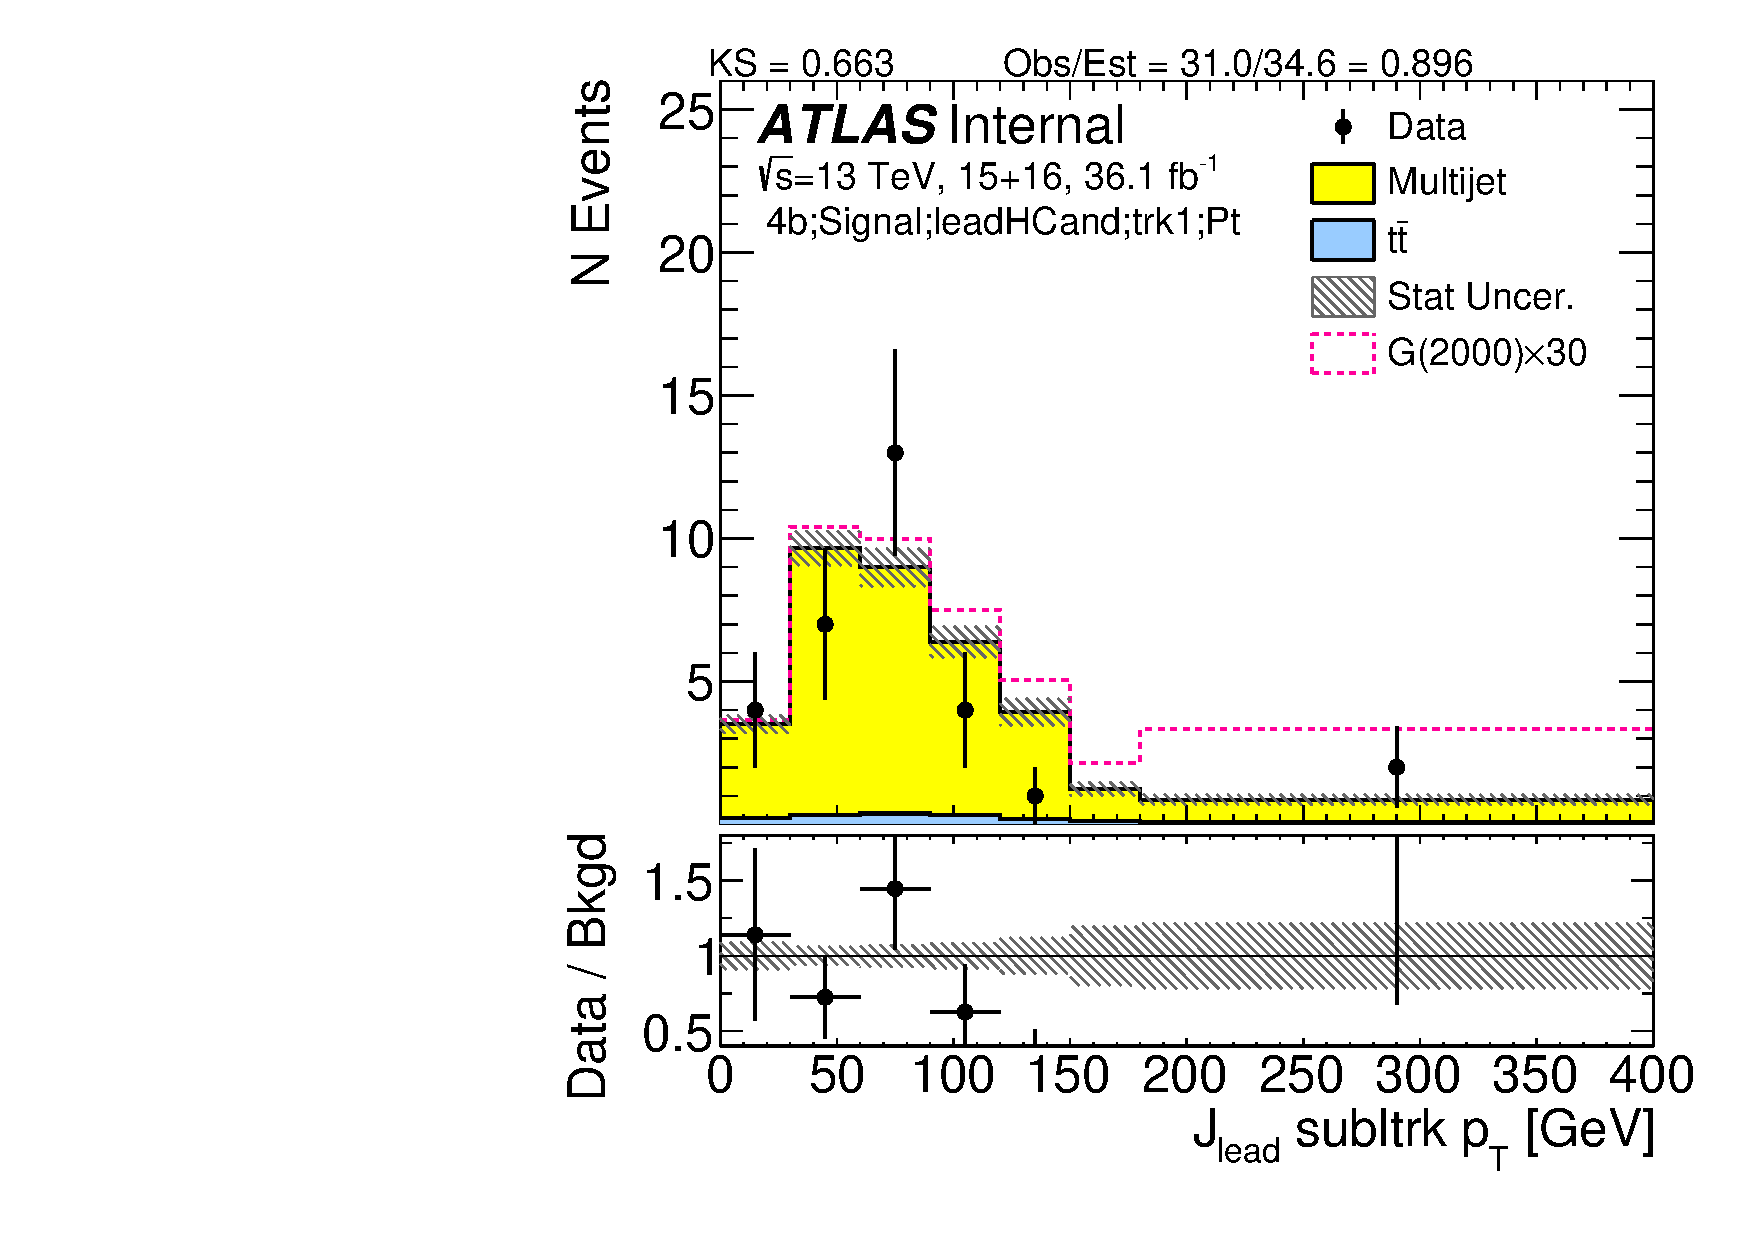
\includegraphics[angle=270, width=0.31\textwidth]{./figures/boosted/Signal/b77_FourTag_Signal_leadHCand_trk1_Pt.pdf}\\
%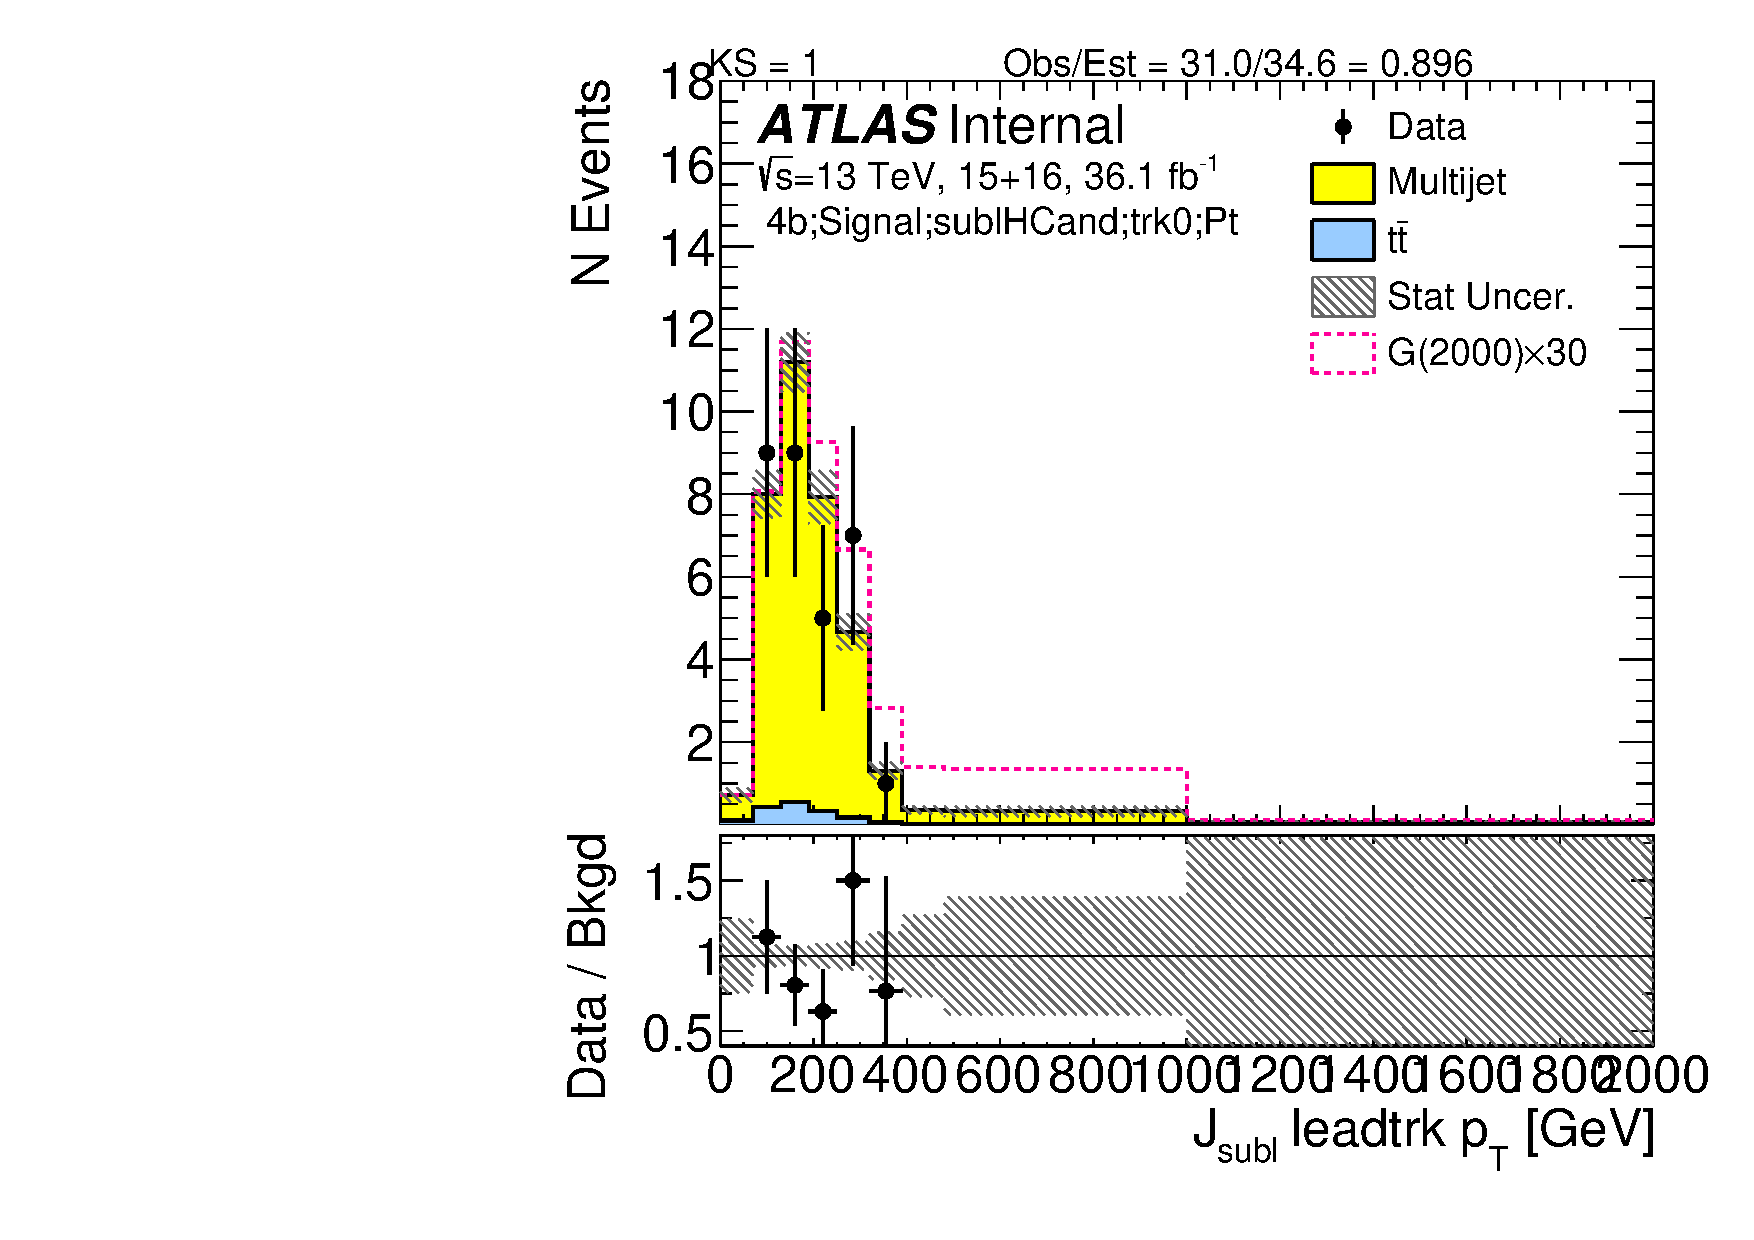
\includegraphics[angle=270, width=0.31\textwidth]{./figures/boosted/Signal/b77_FourTag_Signal_sublHCand_trk0_Pt.pdf}
%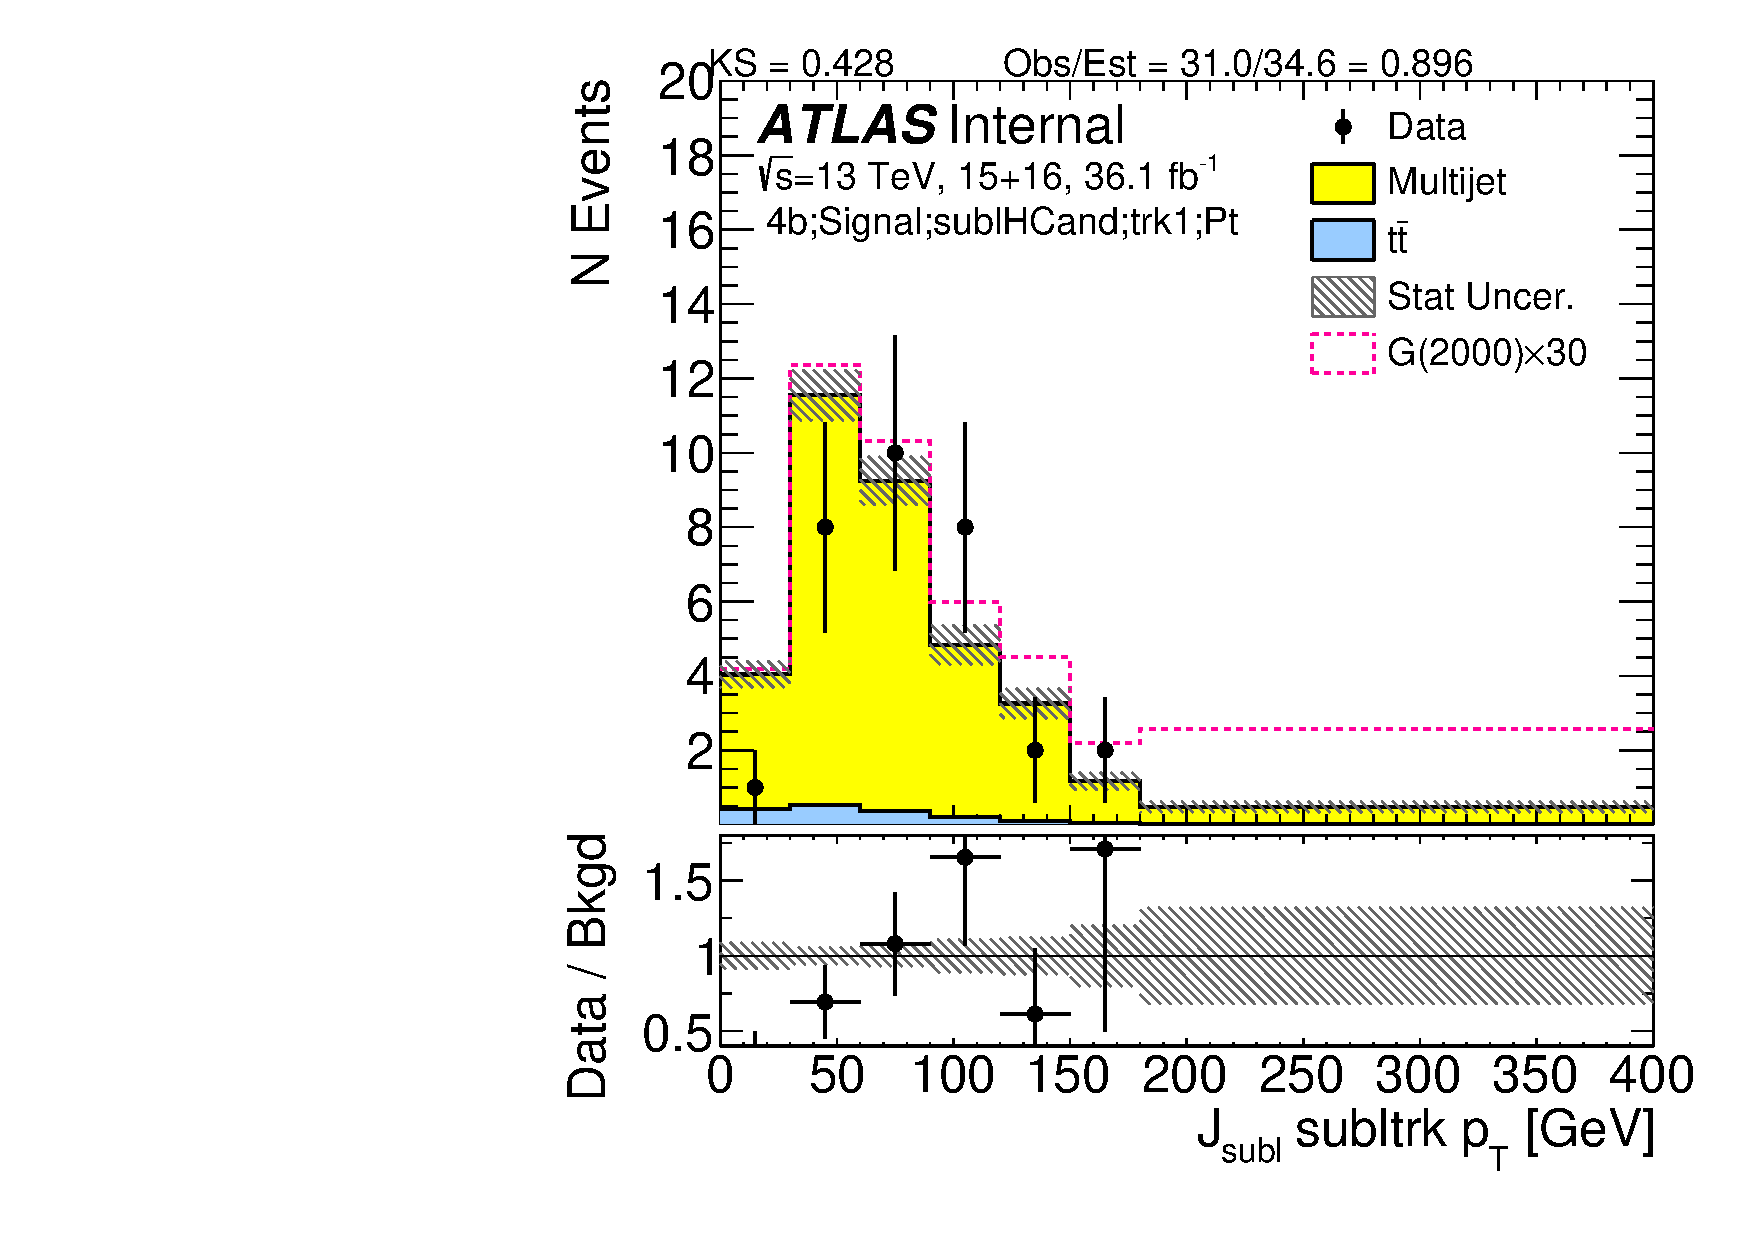
\includegraphics[angle=270, width=0.31\textwidth]{./figures/boosted/Signal/b77_FourTag_Signal_sublHCand_trk1_Pt.pdf}\\
%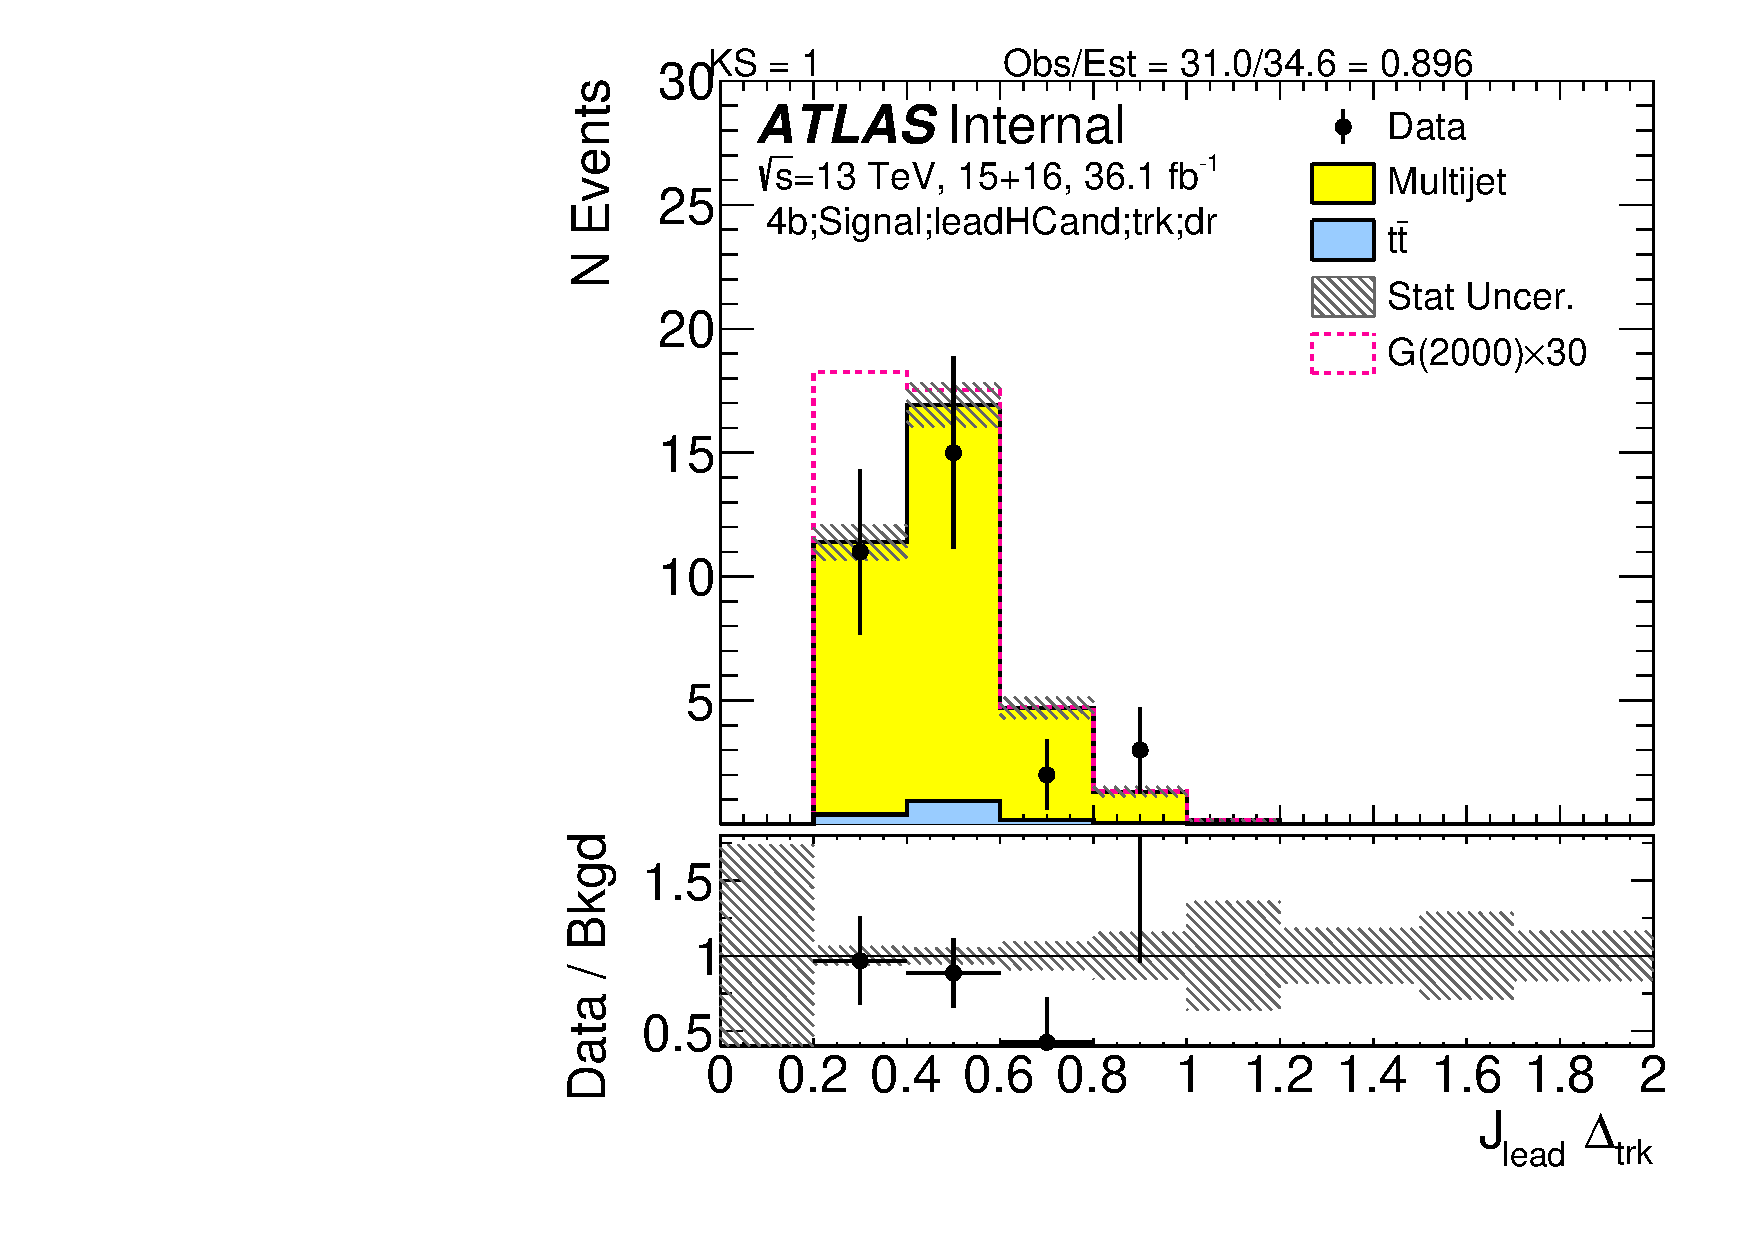
\includegraphics[angle=270, width=0.31\textwidth]{./figures/boosted/Signal/b77_FourTag_Signal_leadHCand_trk_dr.pdf}
%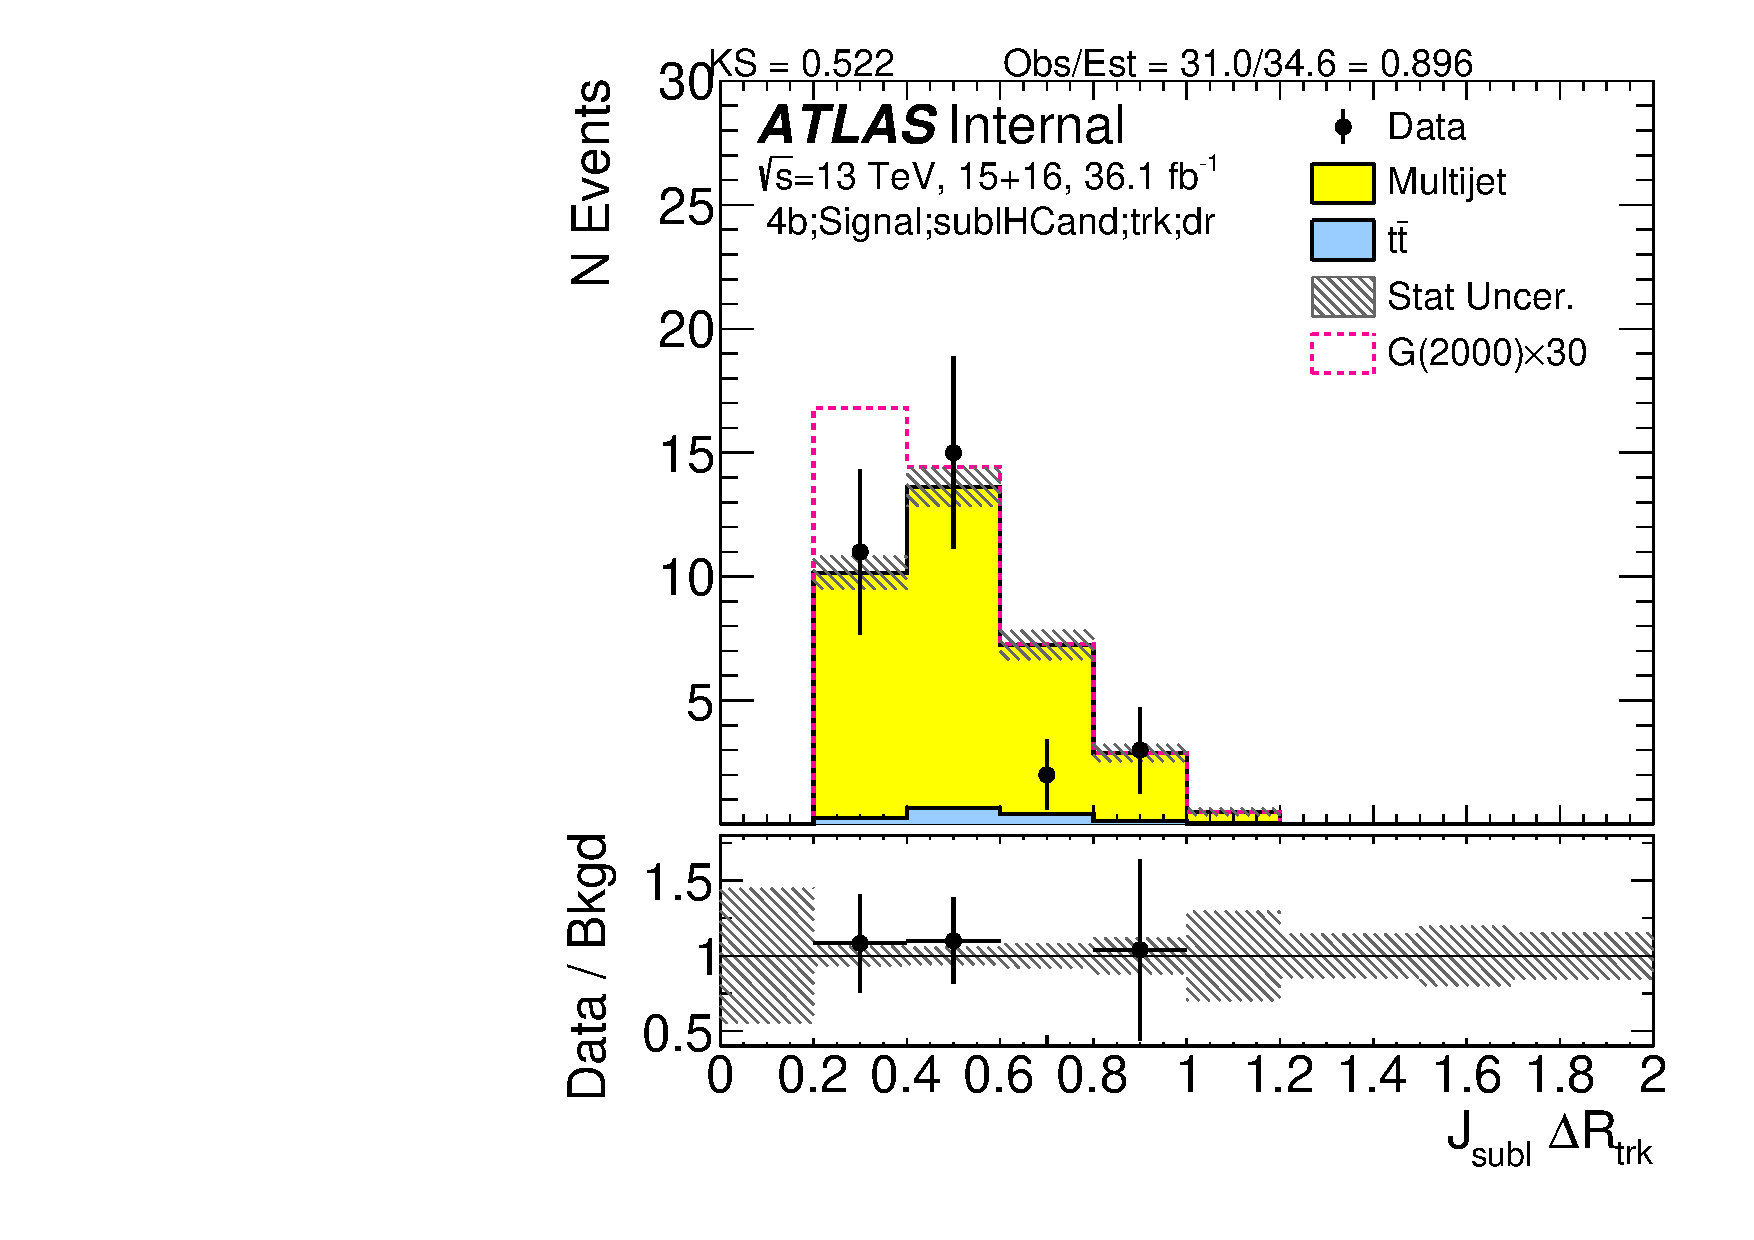
\includegraphics[angle=270, width=0.31\textwidth]{./figures/boosted/Signal/b77_FourTag_Signal_sublHCand_trk_dr.pdf}
  \caption{First two rows show the kinematics of the lead (left) and sub-lead (right) small-$R$ track jets associated to the lead (first-row) and sub-lead (second-row) large-$R$ jet in data and prediction in the signal region after requiring 4 $b$-tags. Third row shows the $\Delta R$ between two leading small-$R$ track-jets associated to the leading (left) and sub-leading (right) large-$R$ jet.  }
  \label{fig:boosted-4b-signal-ak2}
\end{center}
\end{figure*}


\begin{figure*}[htbp!]
\begin{center}
%\includegraphics[angle=270, width=0.31\textwidth]{./figures/boosted/Signal/b77_FourTag_Signal_mHH_l.pdf}
%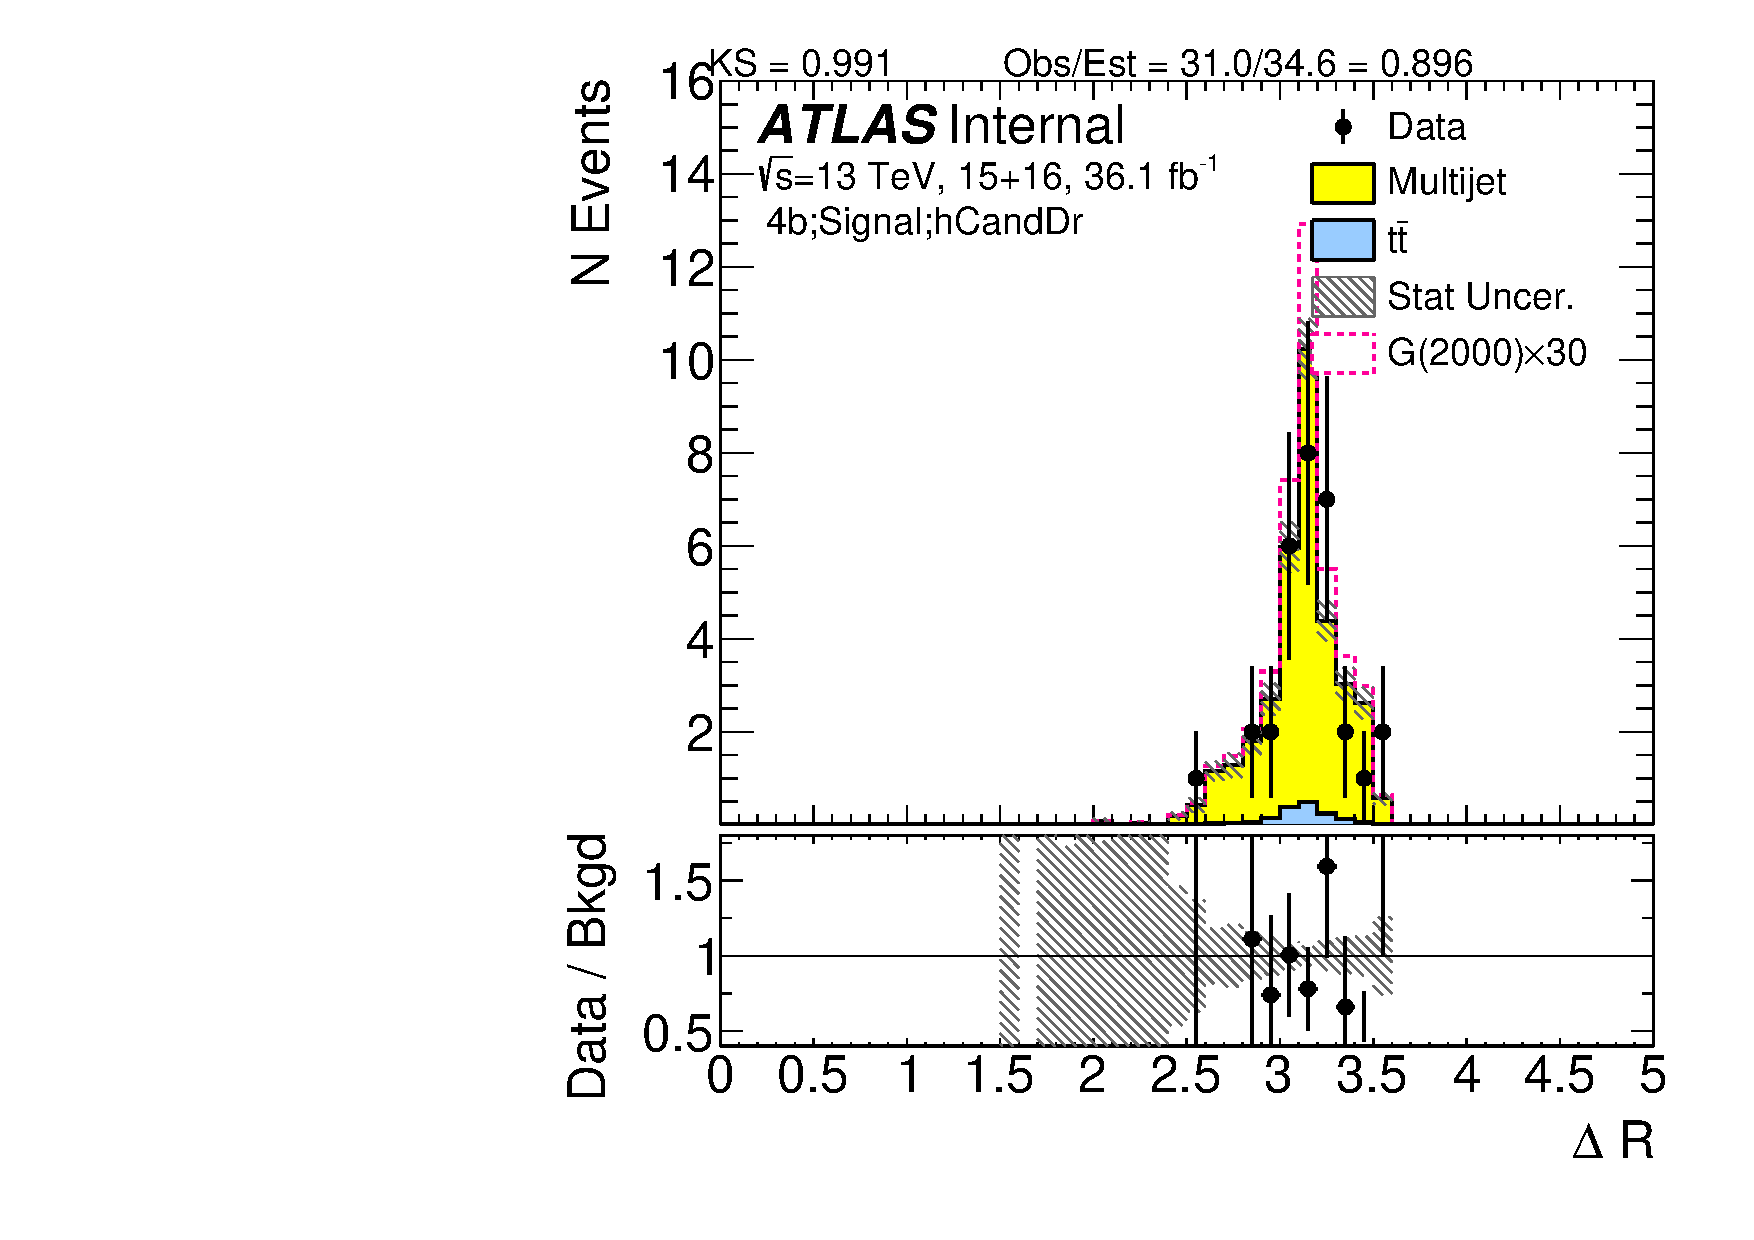
\includegraphics[angle=270, width=0.31\textwidth]{./figures/boosted/Signal/b77_FourTag_Signal_hCandDr.pdf}\\
%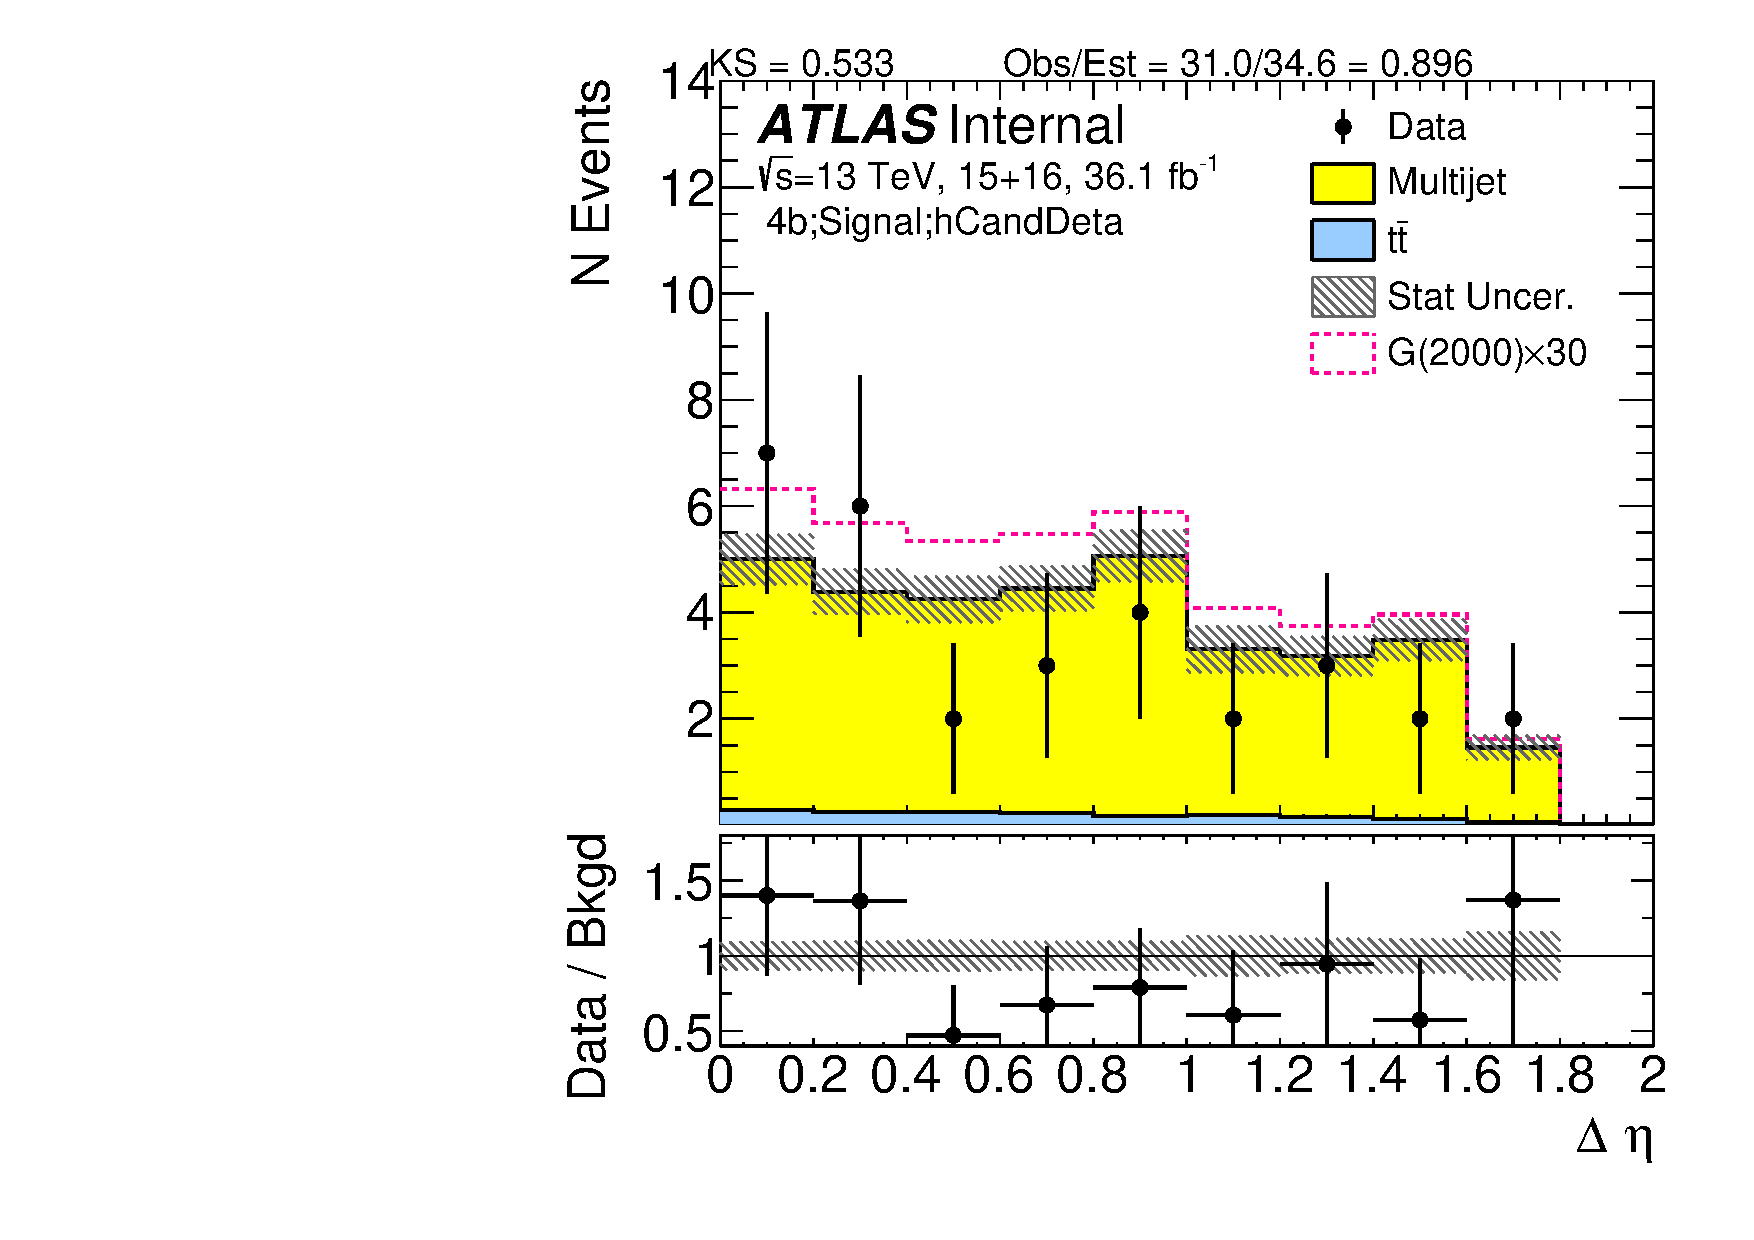
\includegraphics[angle=270, width=0.31\textwidth]{./figures/boosted/Signal/b77_FourTag_Signal_hCandDeta.pdf}
%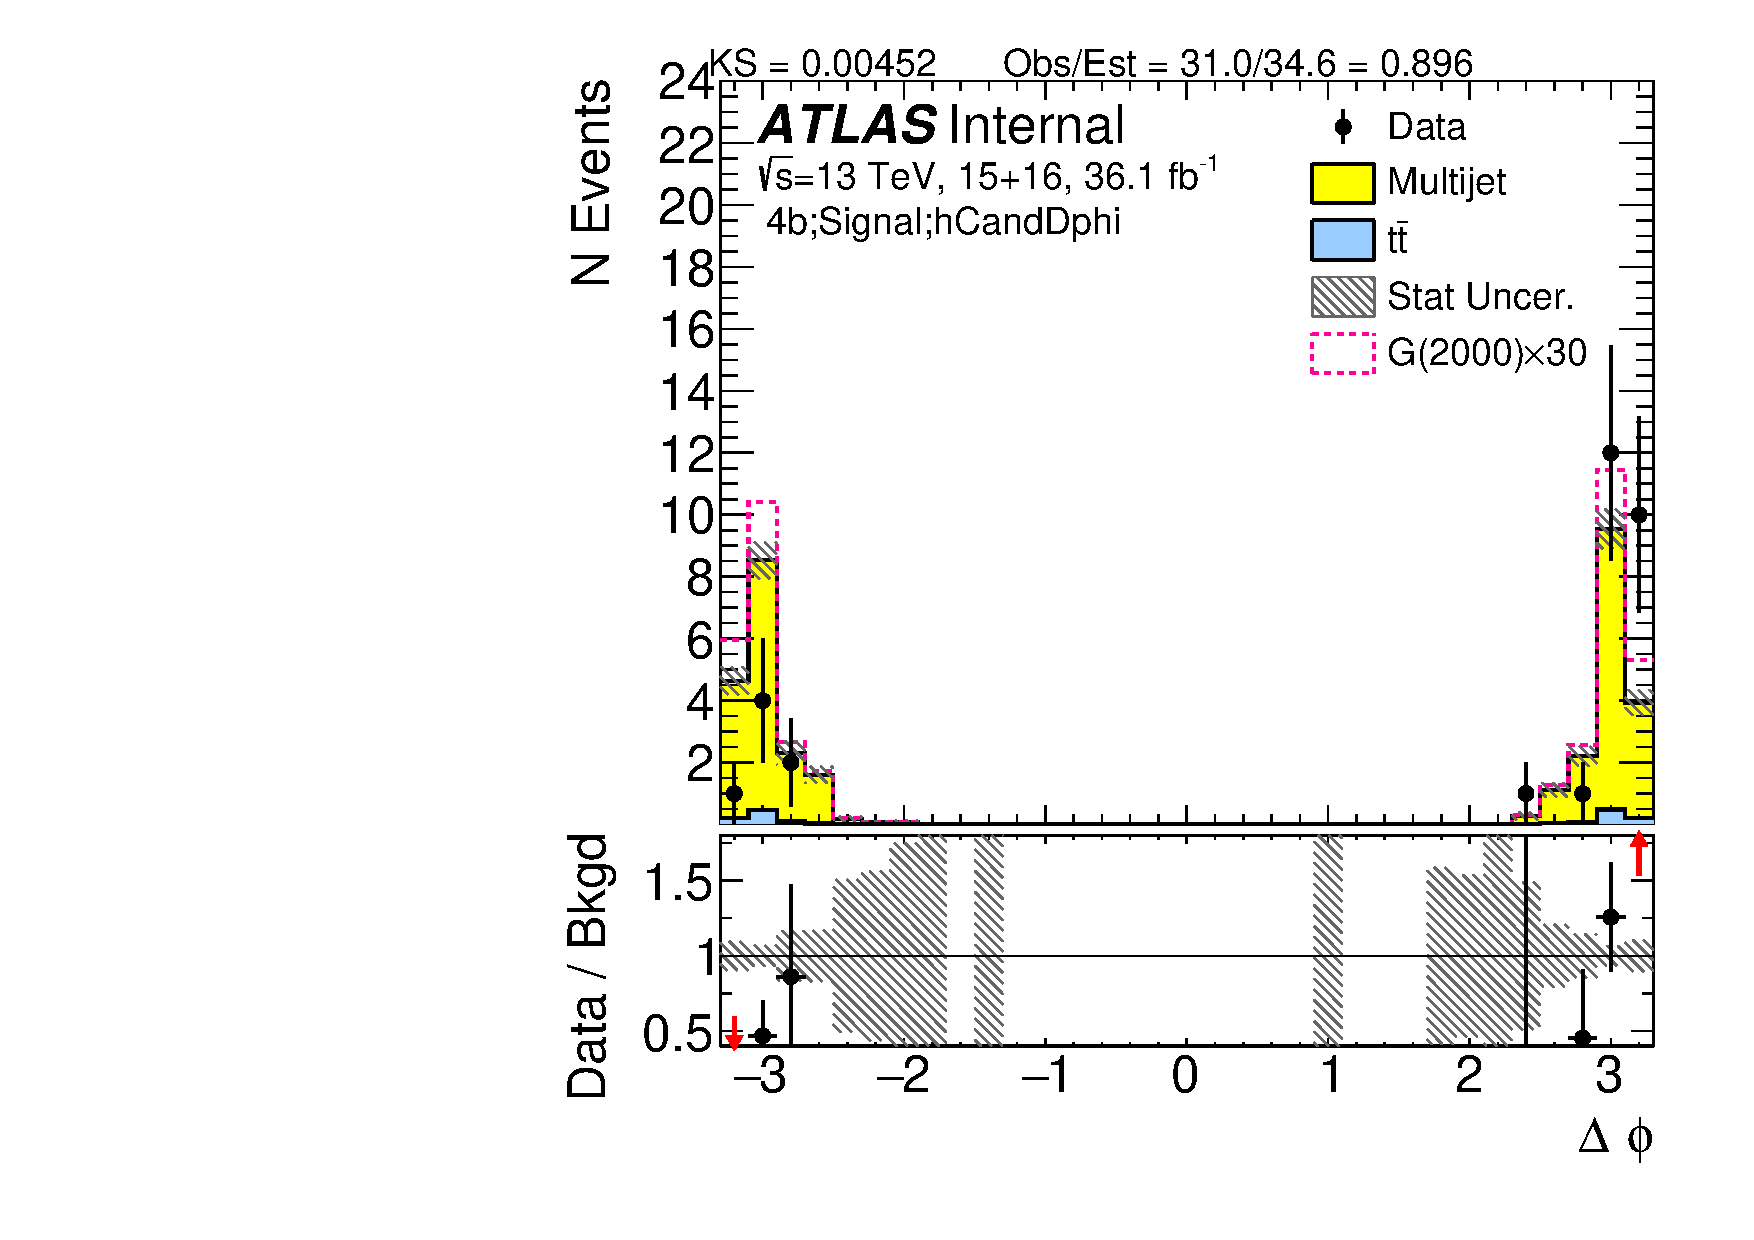
\includegraphics[angle=270, width=0.31\textwidth]{./figures/boosted/Signal/b77_FourTag_Signal_hCandDphi.pdf}
  \caption{Kinematics of the large-$R$ jet system in data and prediction in the signal region after requiring 4 $b$-tags.  }
  \label{fig:boosted-4b-signal-ak10-system}
\end{center}
\end{figure*}

\clearpage

\begin{figure*}[htbp!]
\begin{center}
%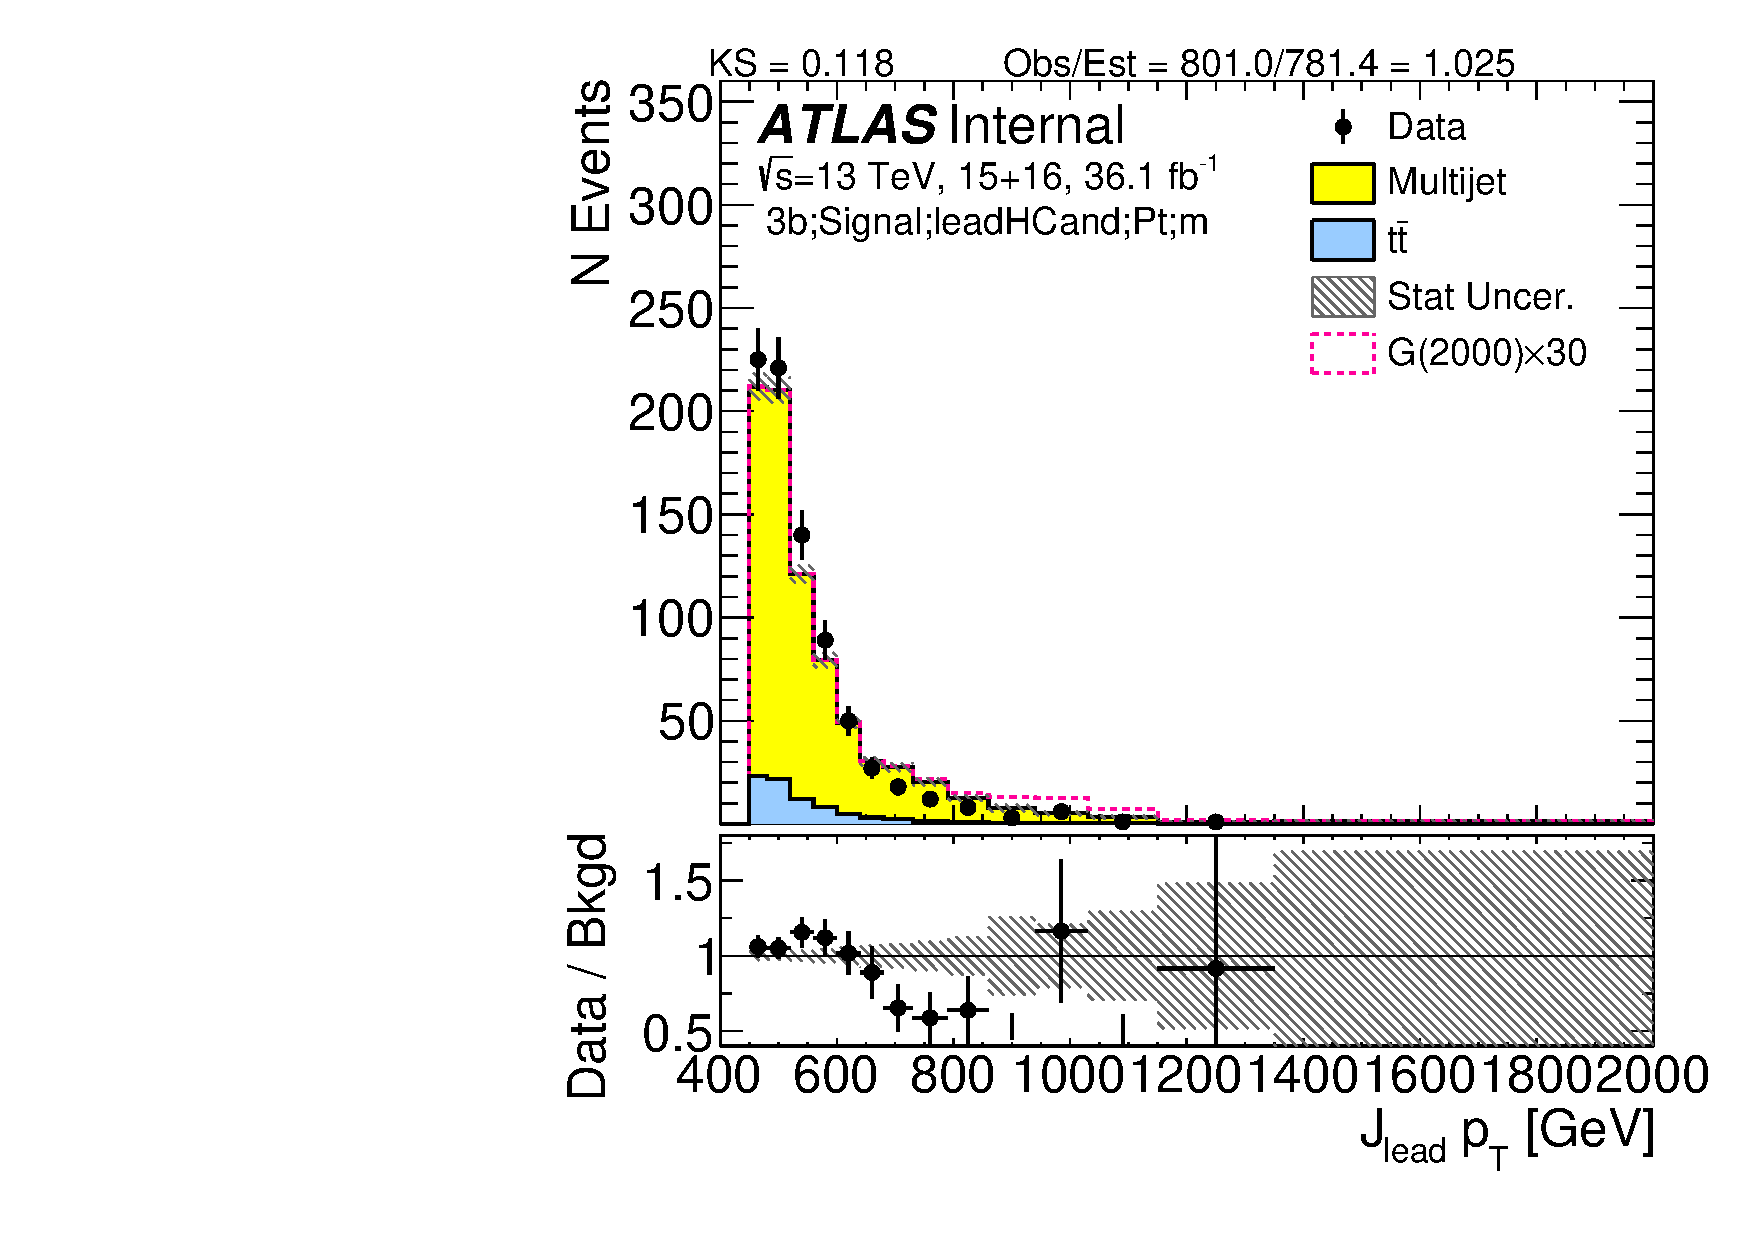
\includegraphics[angle=270, width=0.31\textwidth]{./figures/boosted/Signal/b77_ThreeTag_Signal_leadHCand_Pt_m.pdf}
%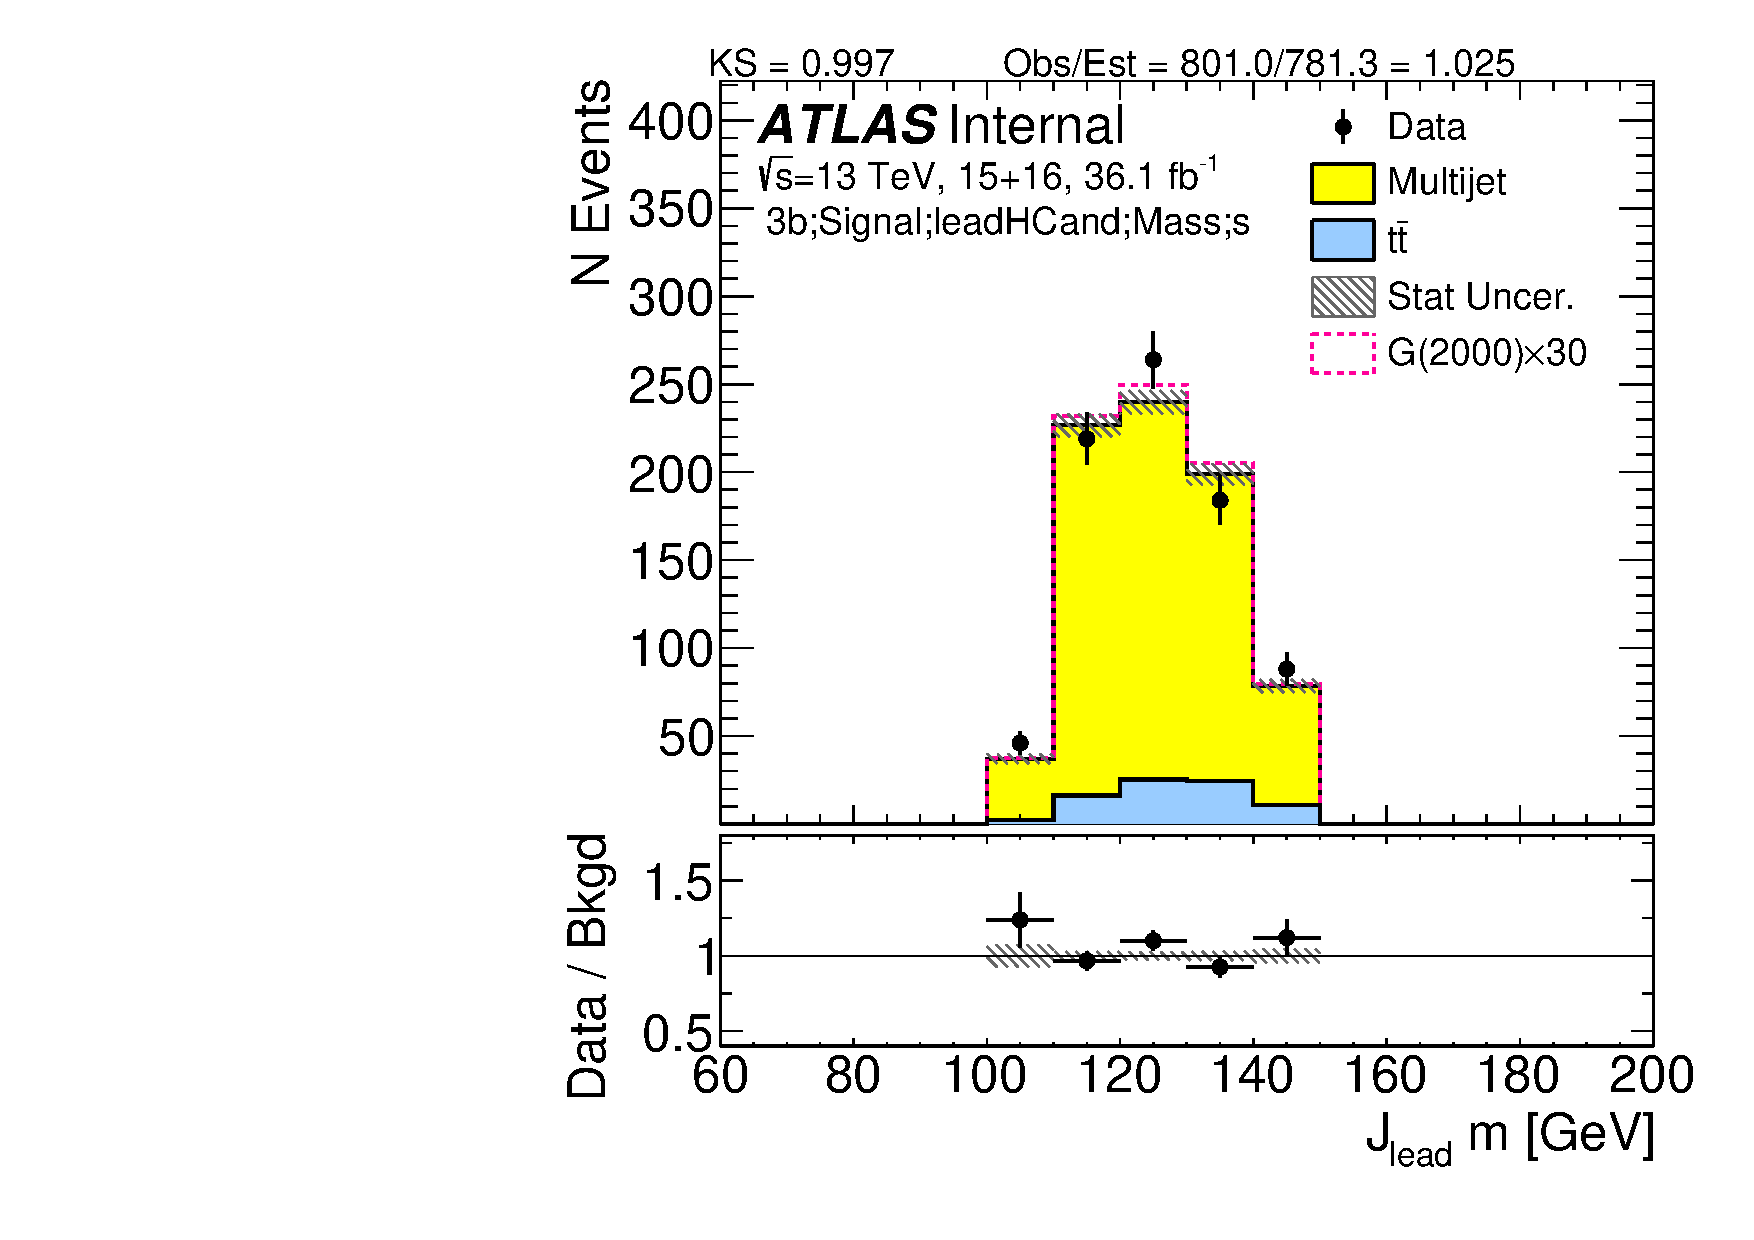
\includegraphics[angle=270, width=0.31\textwidth]{./figures/boosted/Signal/b77_ThreeTag_Signal_leadHCand_Mass_s.pdf}\\
%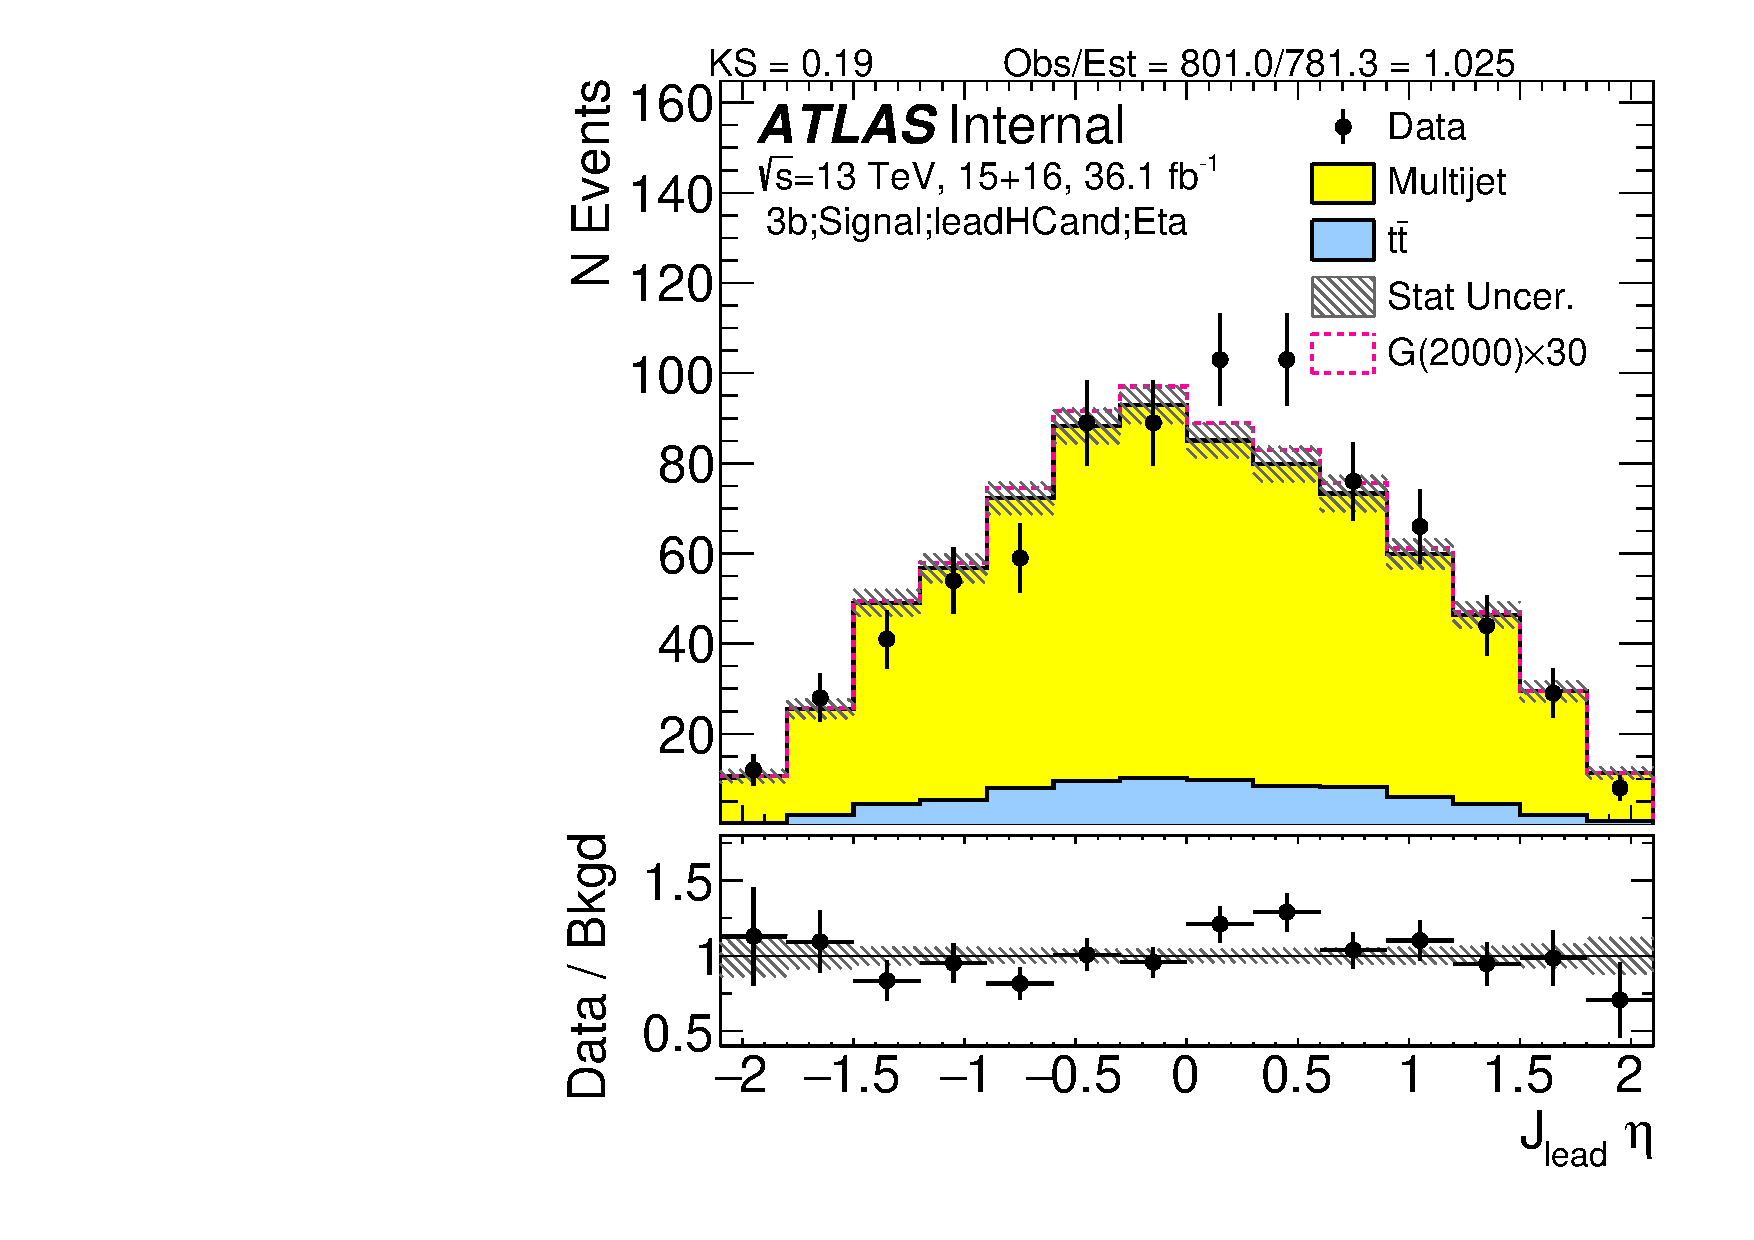
\includegraphics[angle=270, width=0.31\textwidth]{./figures/boosted/Signal/b77_ThreeTag_Signal_leadHCand_Eta.pdf}
%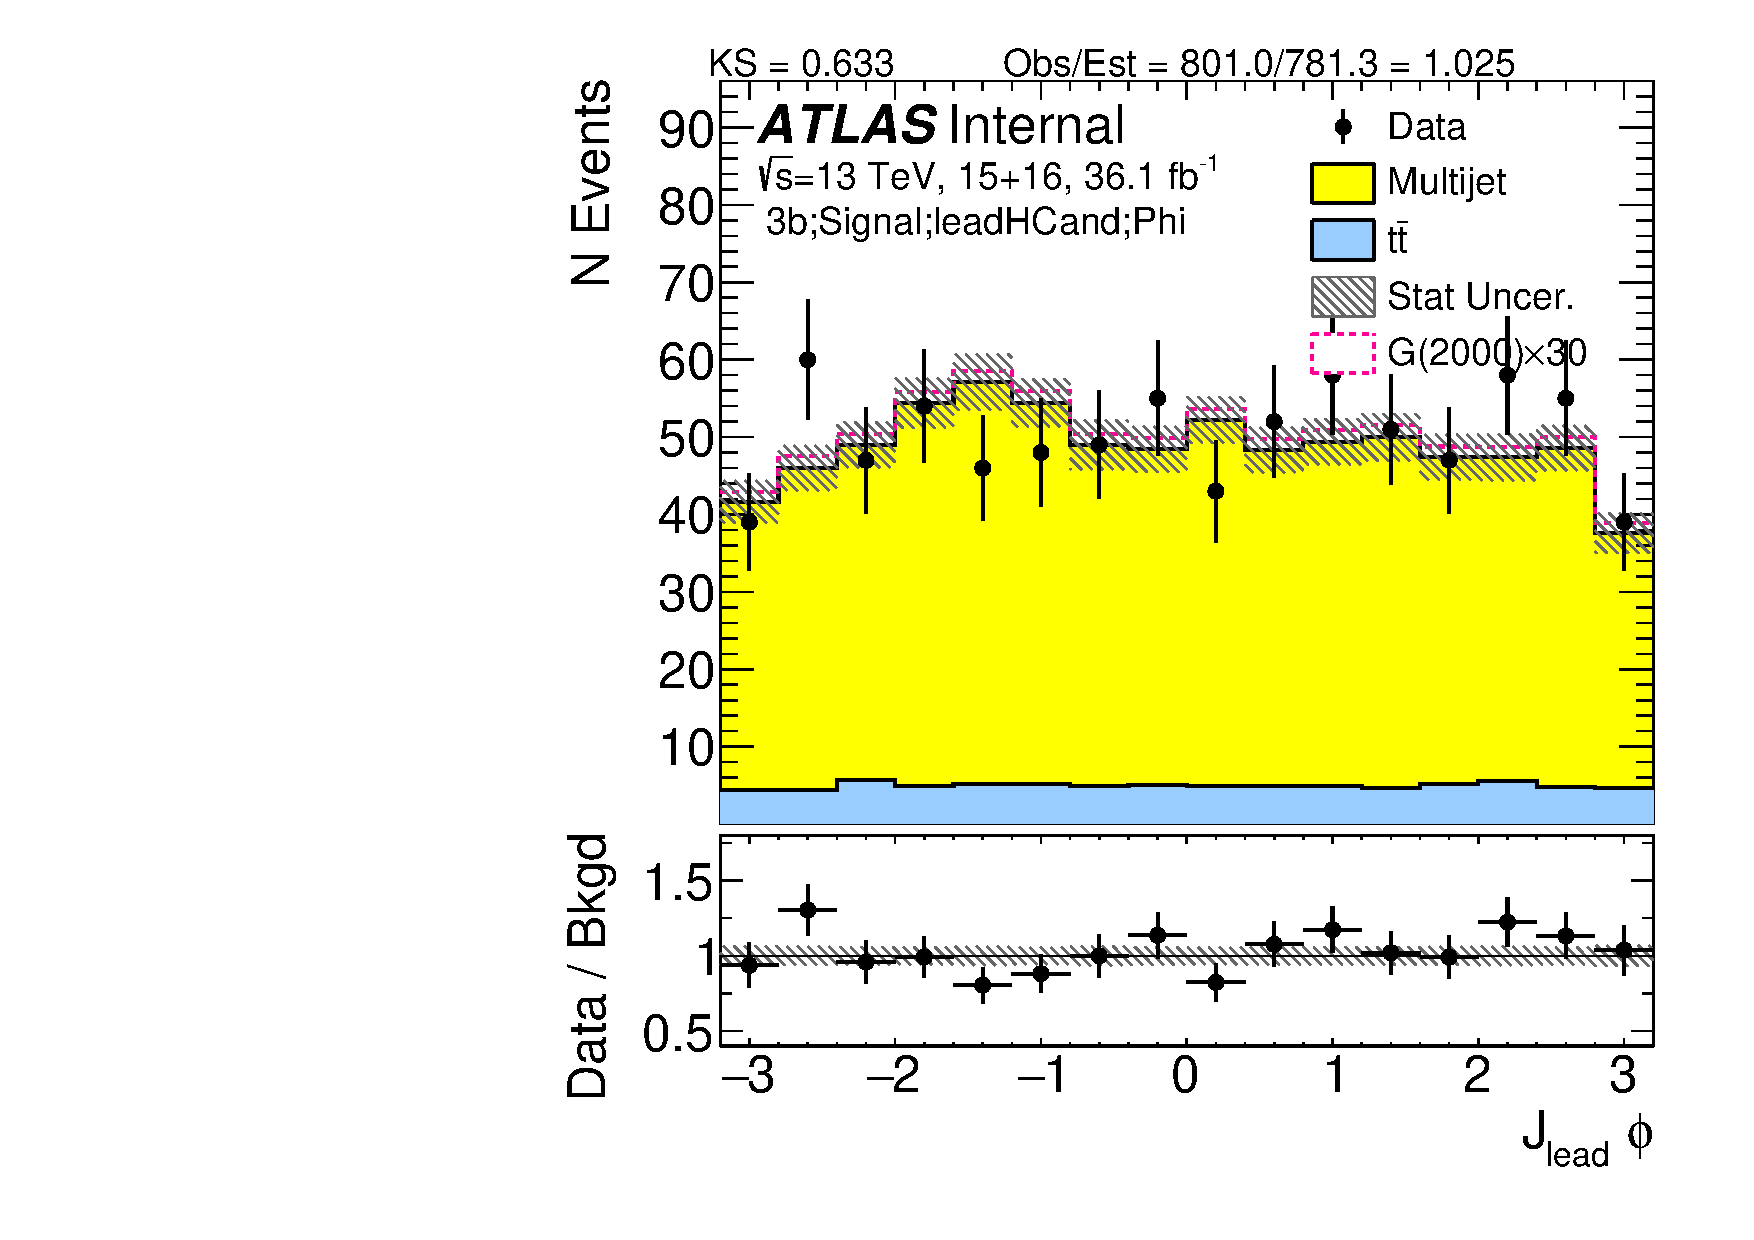
\includegraphics[angle=270, width=0.31\textwidth]{./figures/boosted/Signal/b77_ThreeTag_Signal_leadHCand_Phi.pdf}
  \caption{Kinematics of the lead large-$R$ jet in data and prediction in the signal region after requiring 3 $b$-tags. }
  \label{fig:boosted-3b-signal-ak10-lead}
\end{center}
\end{figure*}

\begin{figure*}[htbp!]
\begin{center}
%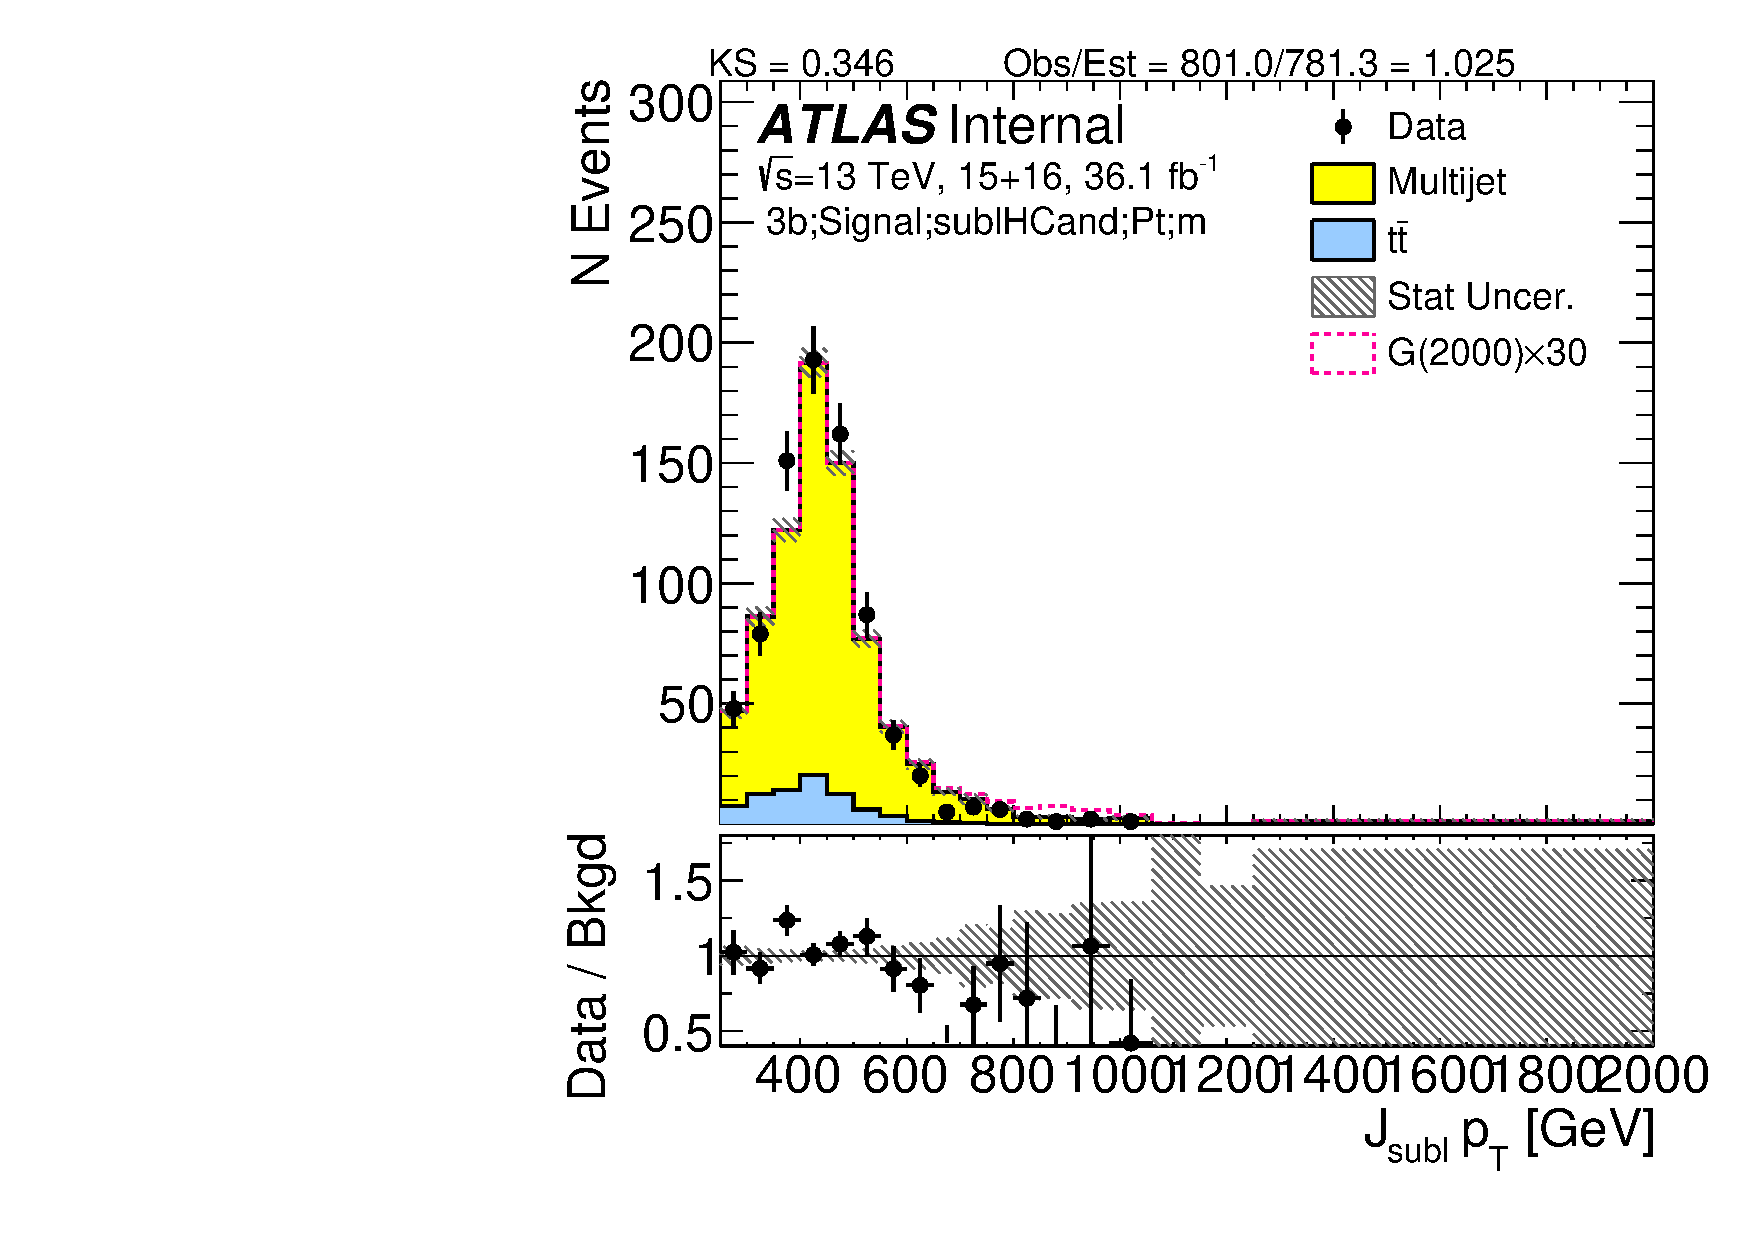
\includegraphics[angle=270, width=0.31\textwidth]{./figures/boosted/Signal/b77_ThreeTag_Signal_sublHCand_Pt_m.pdf}
%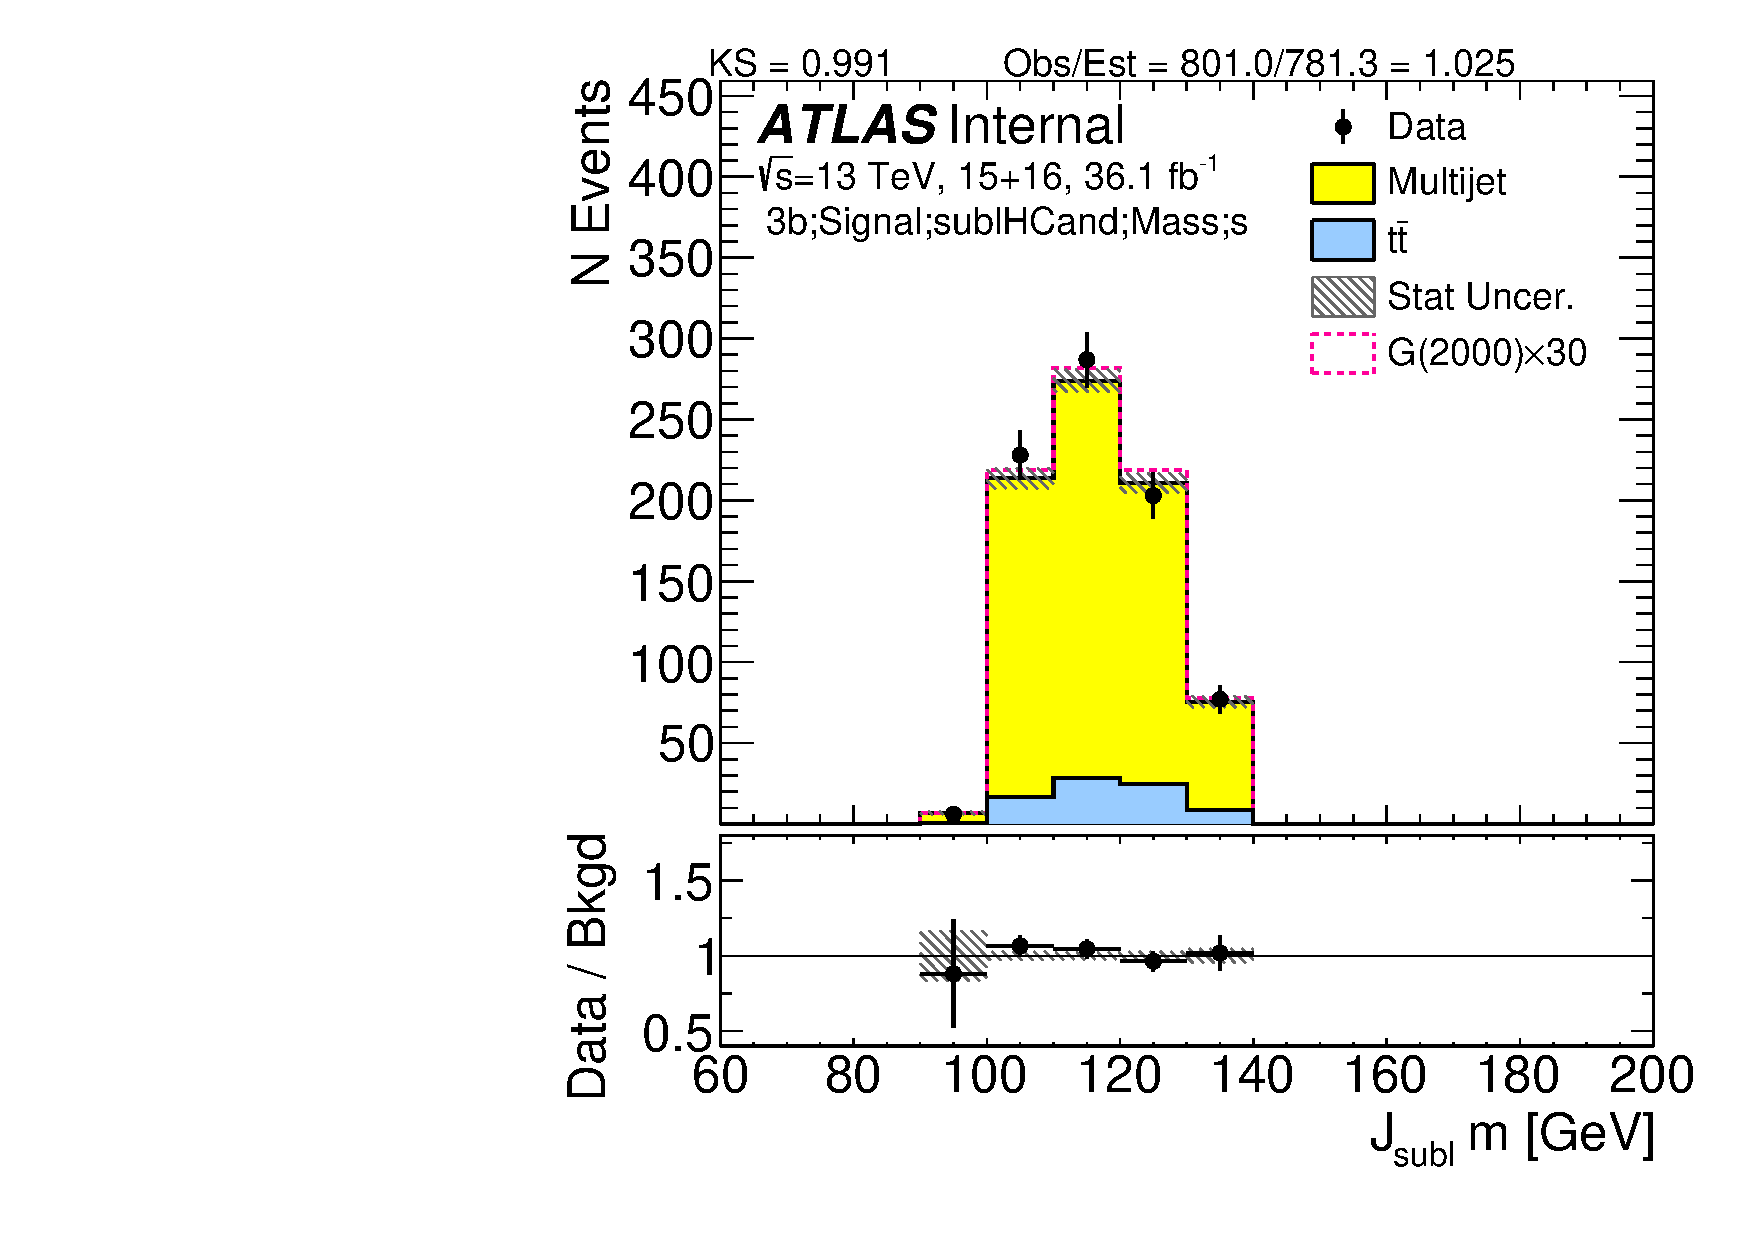
\includegraphics[angle=270, width=0.31\textwidth]{./figures/boosted/Signal/b77_ThreeTag_Signal_sublHCand_Mass_s.pdf}\\
%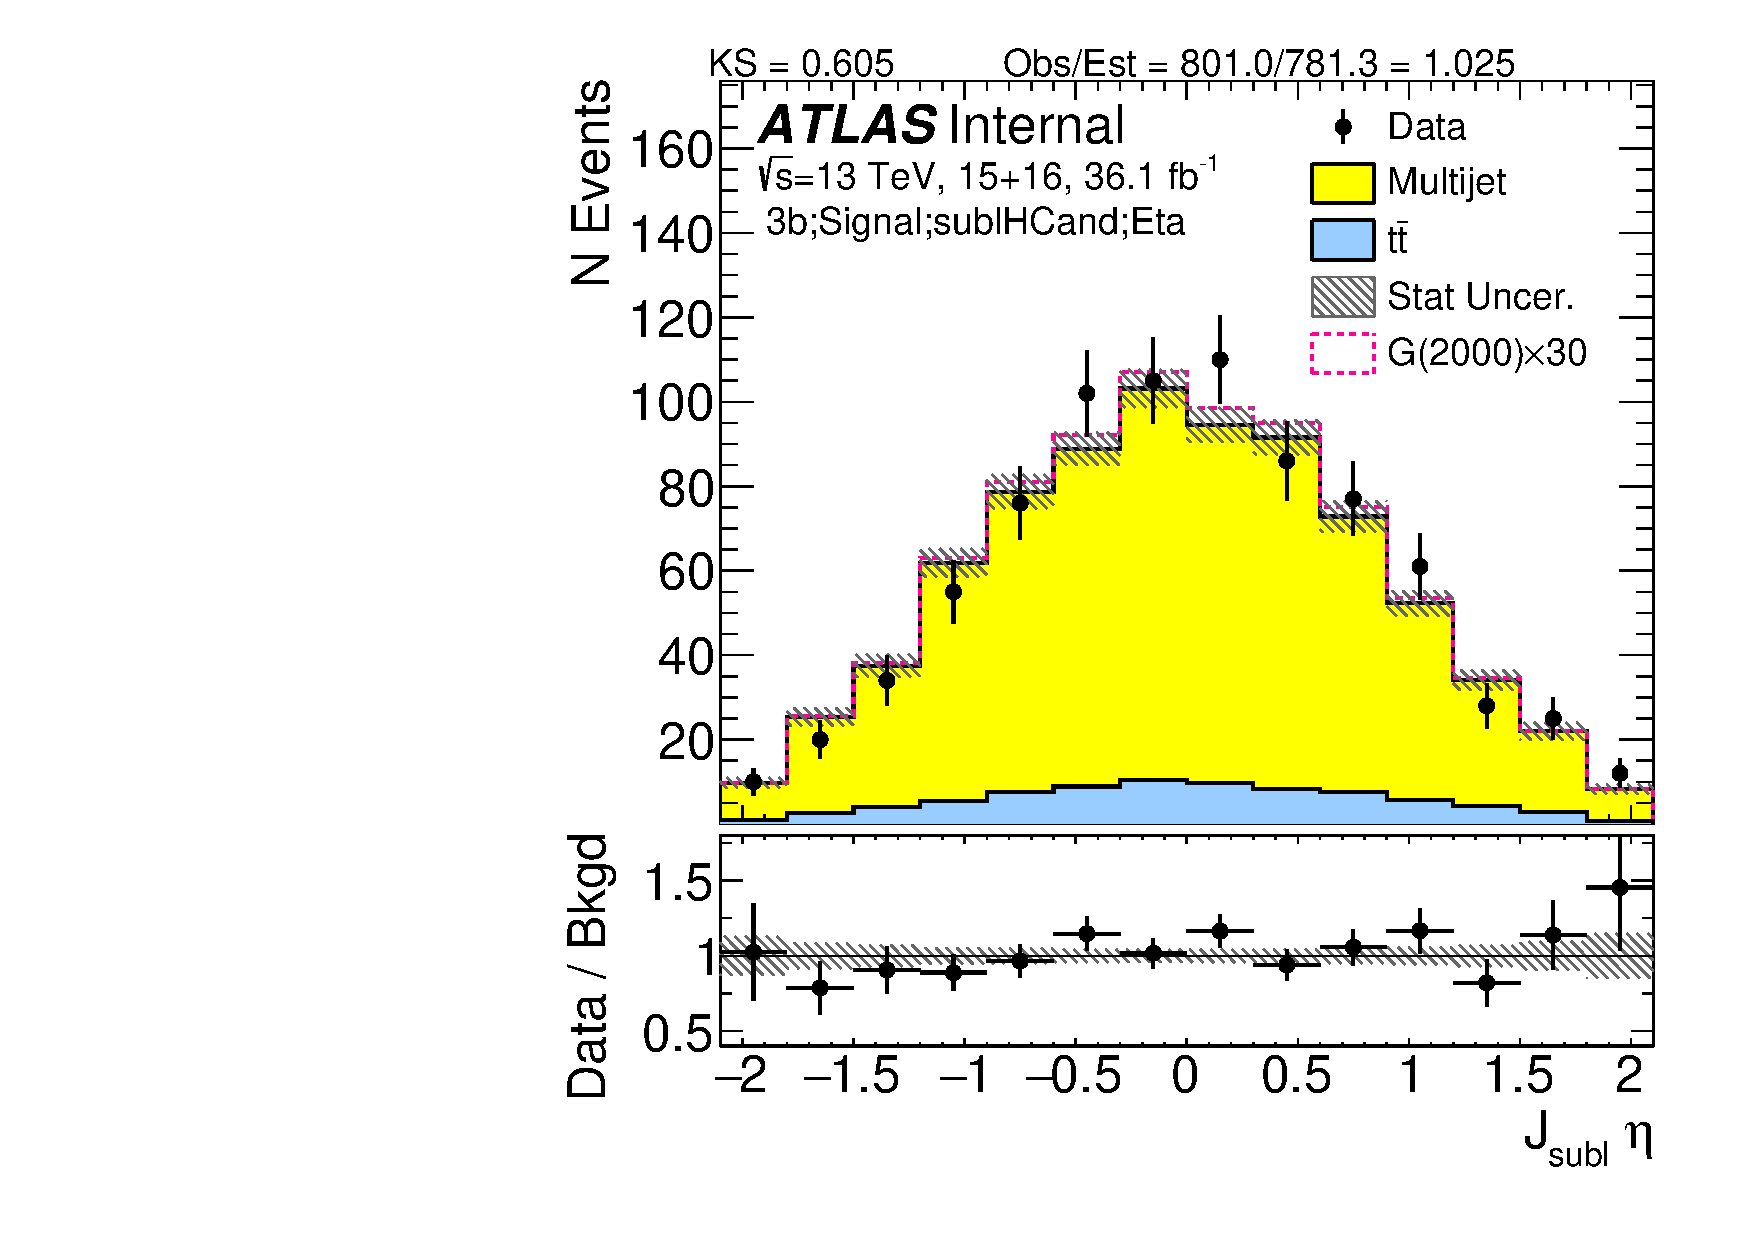
\includegraphics[angle=270, width=0.31\textwidth]{./figures/boosted/Signal/b77_ThreeTag_Signal_sublHCand_Eta.pdf}
%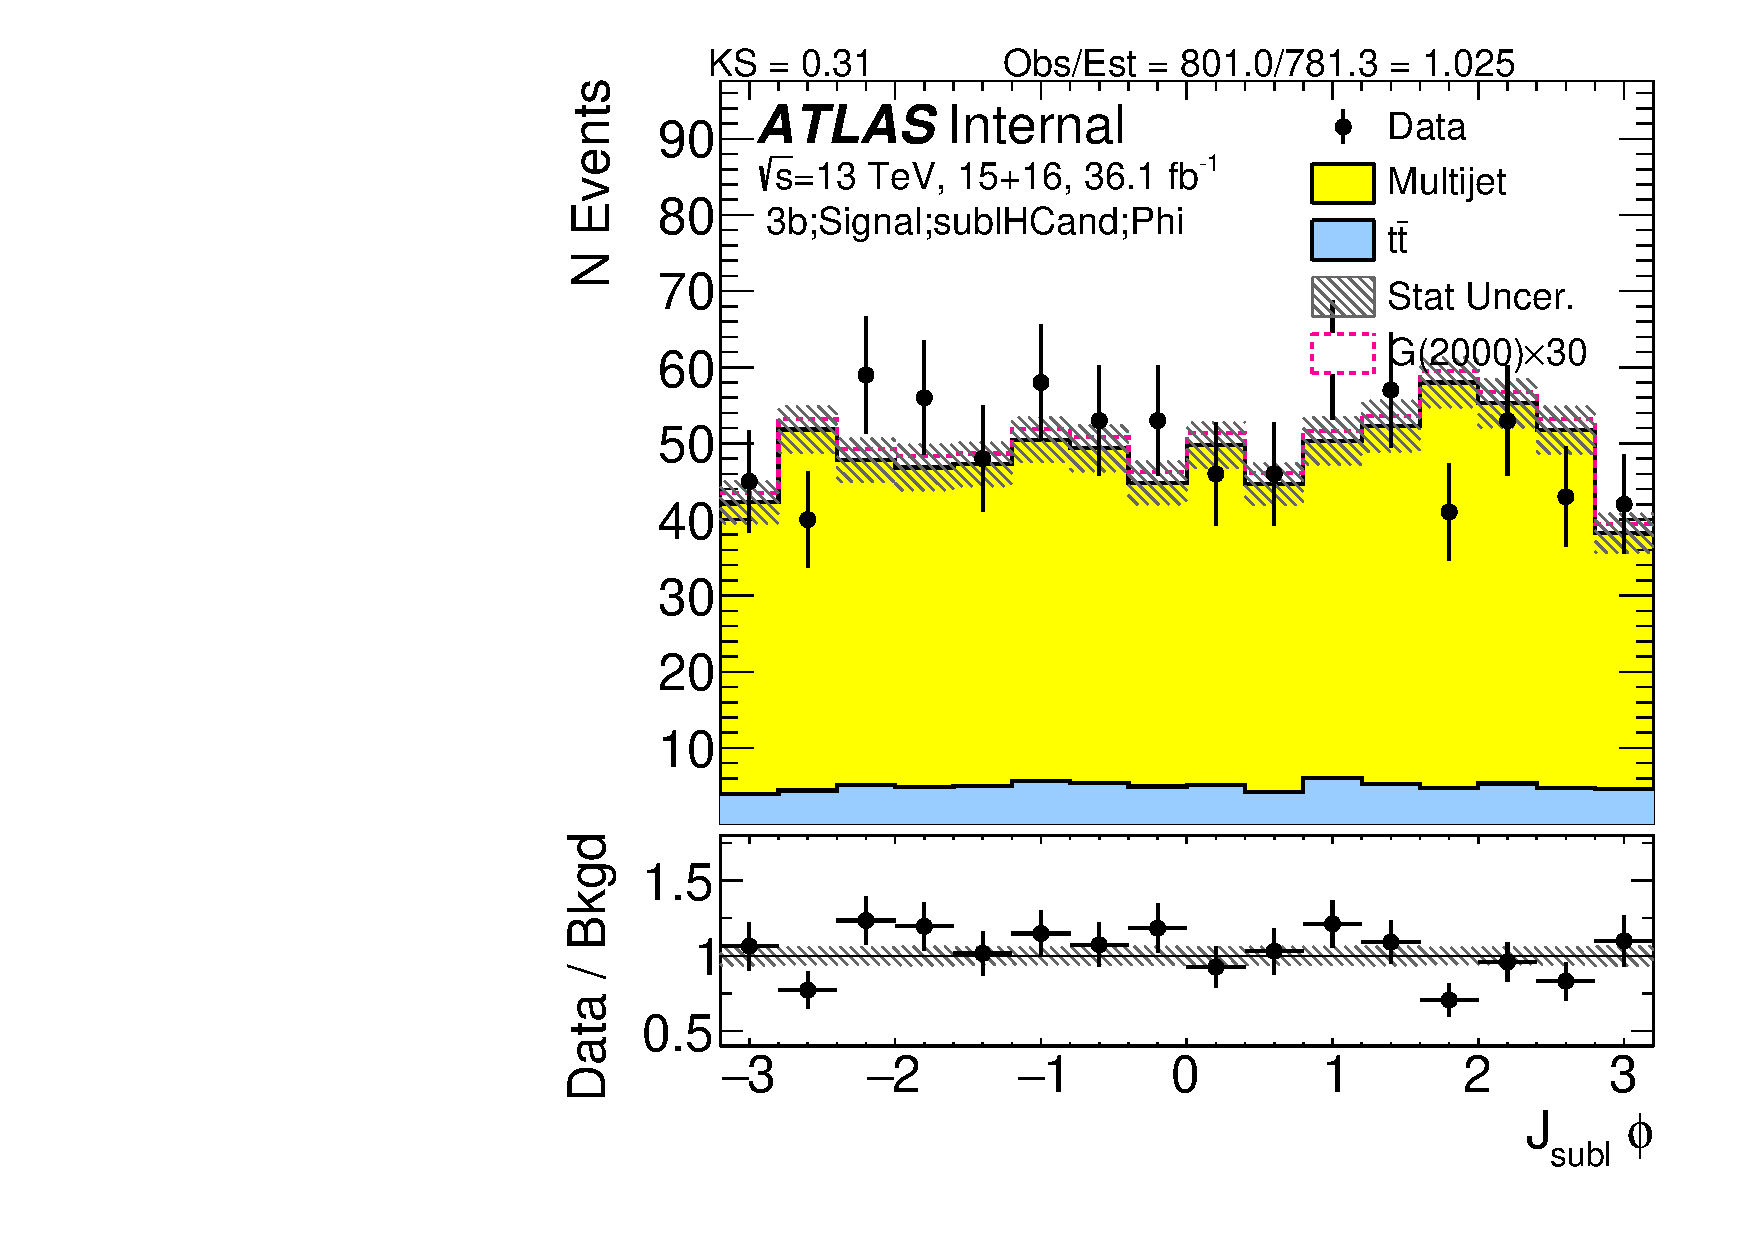
\includegraphics[angle=270, width=0.31\textwidth]{./figures/boosted/Signal/b77_ThreeTag_Signal_sublHCand_Phi.pdf}
  \caption{Kinematics of the sub-lead large-$R$ jet in data and prediction in the signal region after requiring 3 $b$-tags. }
  \label{fig:boosted-3b-signal-ak10-subl}
\end{center}
\end{figure*}

\begin{figure*}[htbp!]
\begin{center}
%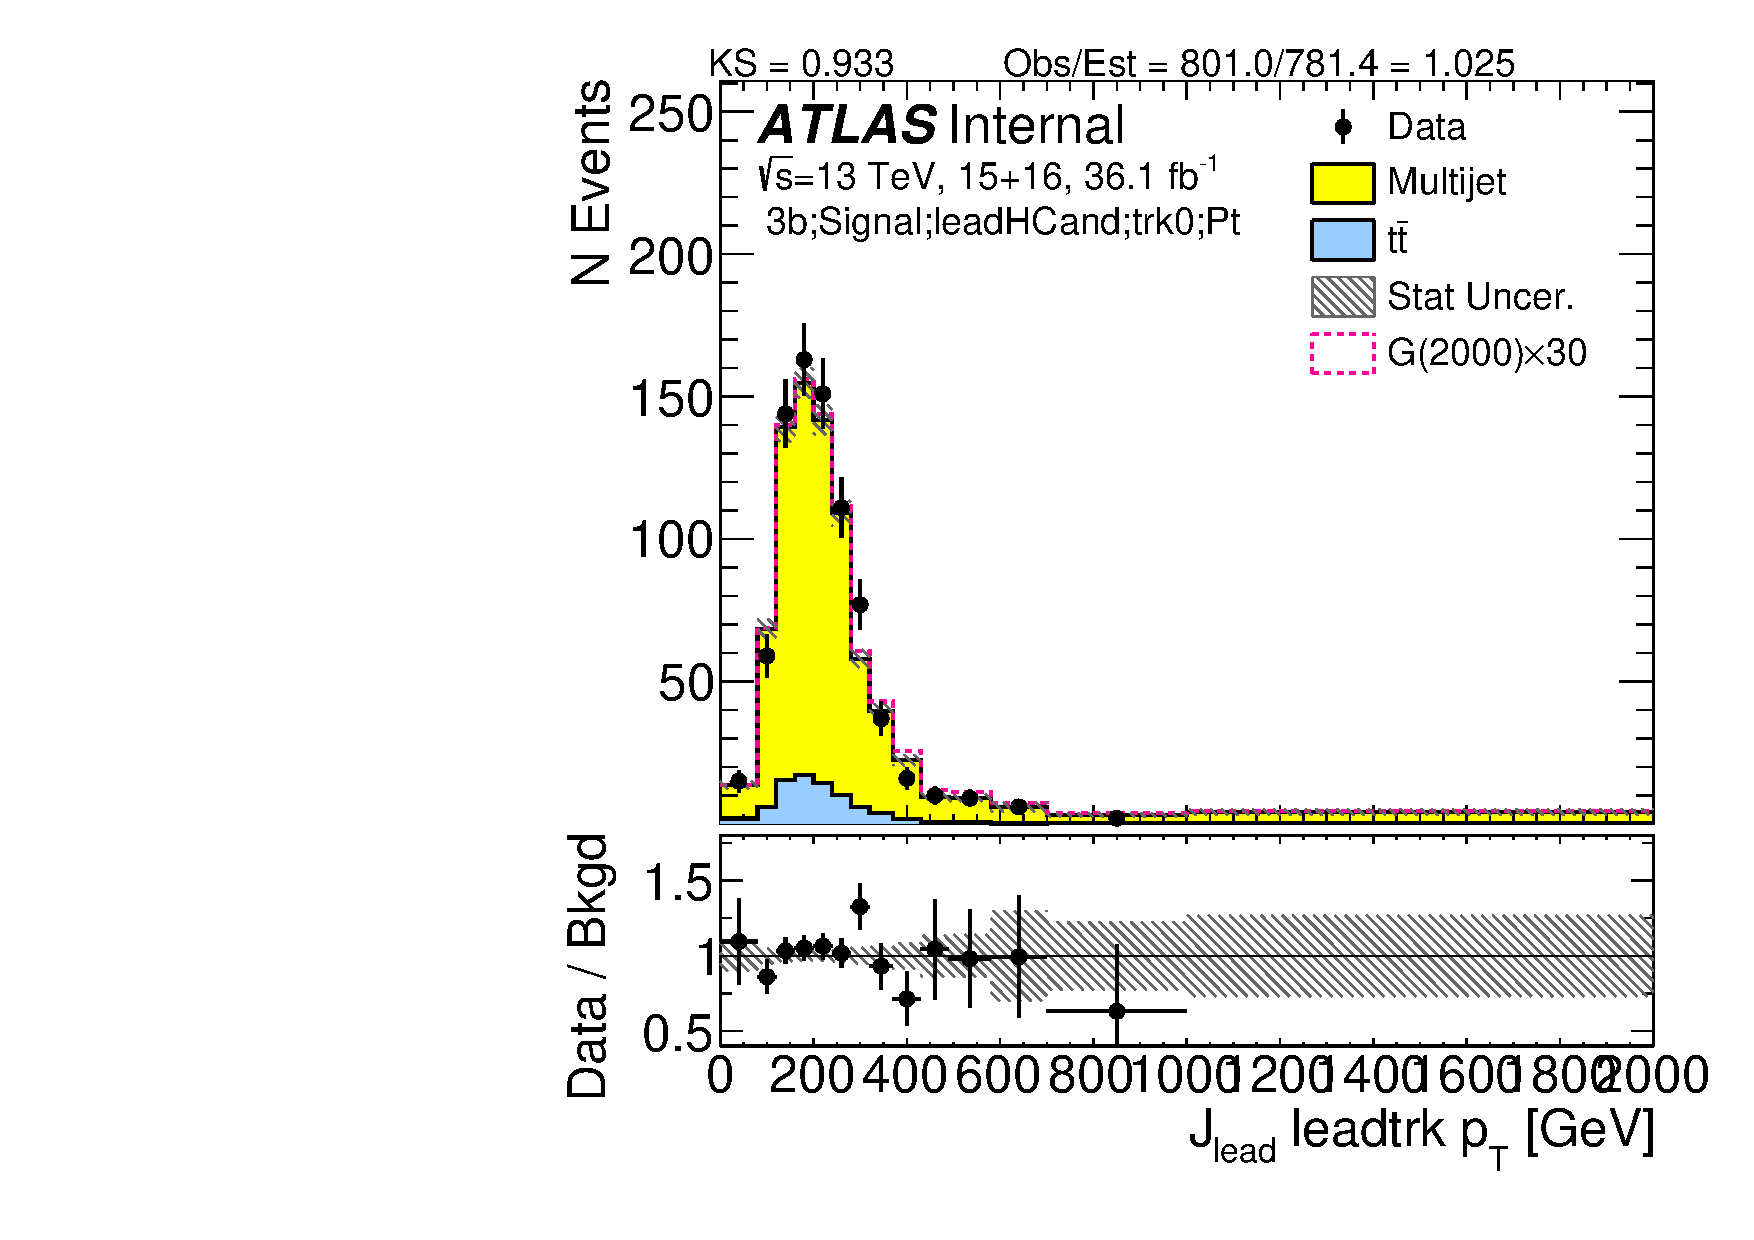
\includegraphics[angle=270, width=0.31\textwidth]{./figures/boosted/Signal/b77_ThreeTag_Signal_leadHCand_trk0_Pt.pdf}
%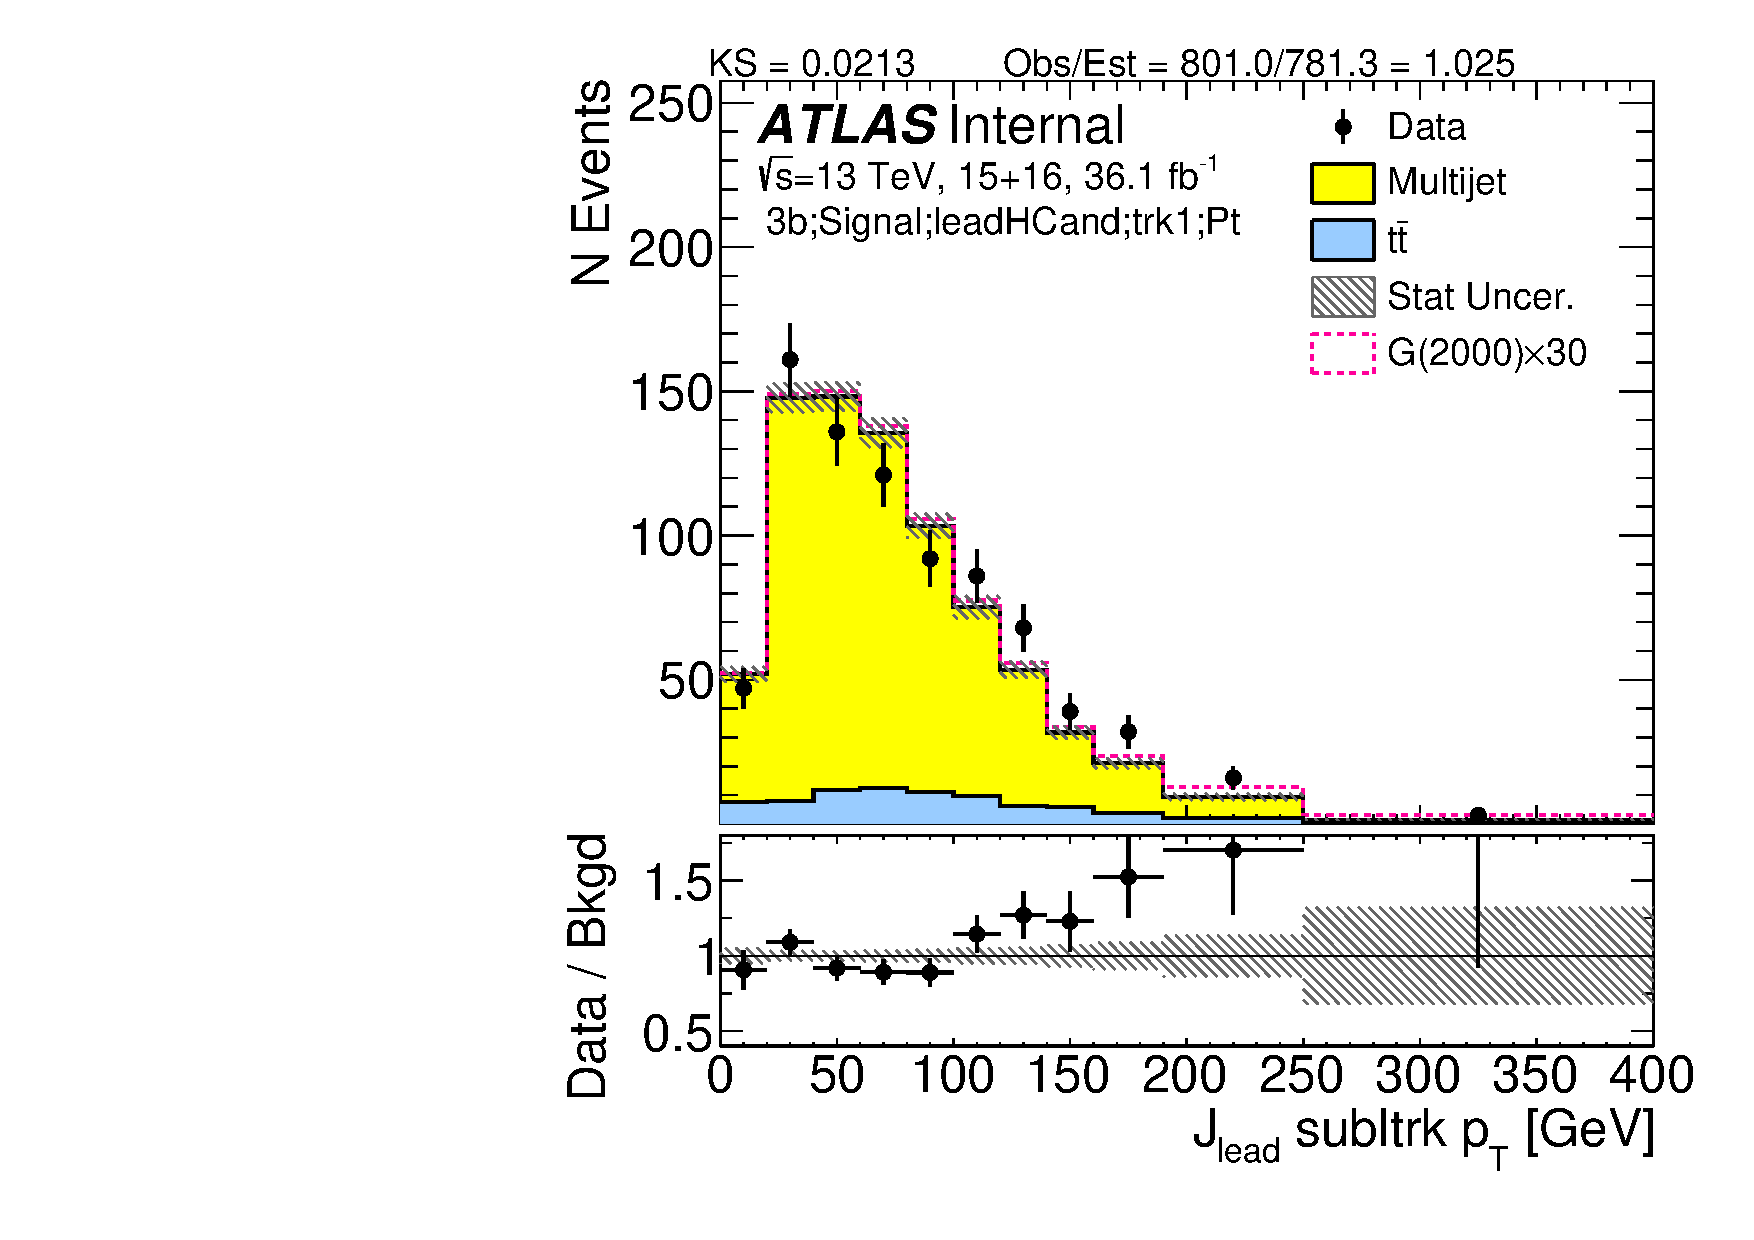
\includegraphics[angle=270, width=0.31\textwidth]{./figures/boosted/Signal/b77_ThreeTag_Signal_leadHCand_trk1_Pt.pdf}\\
%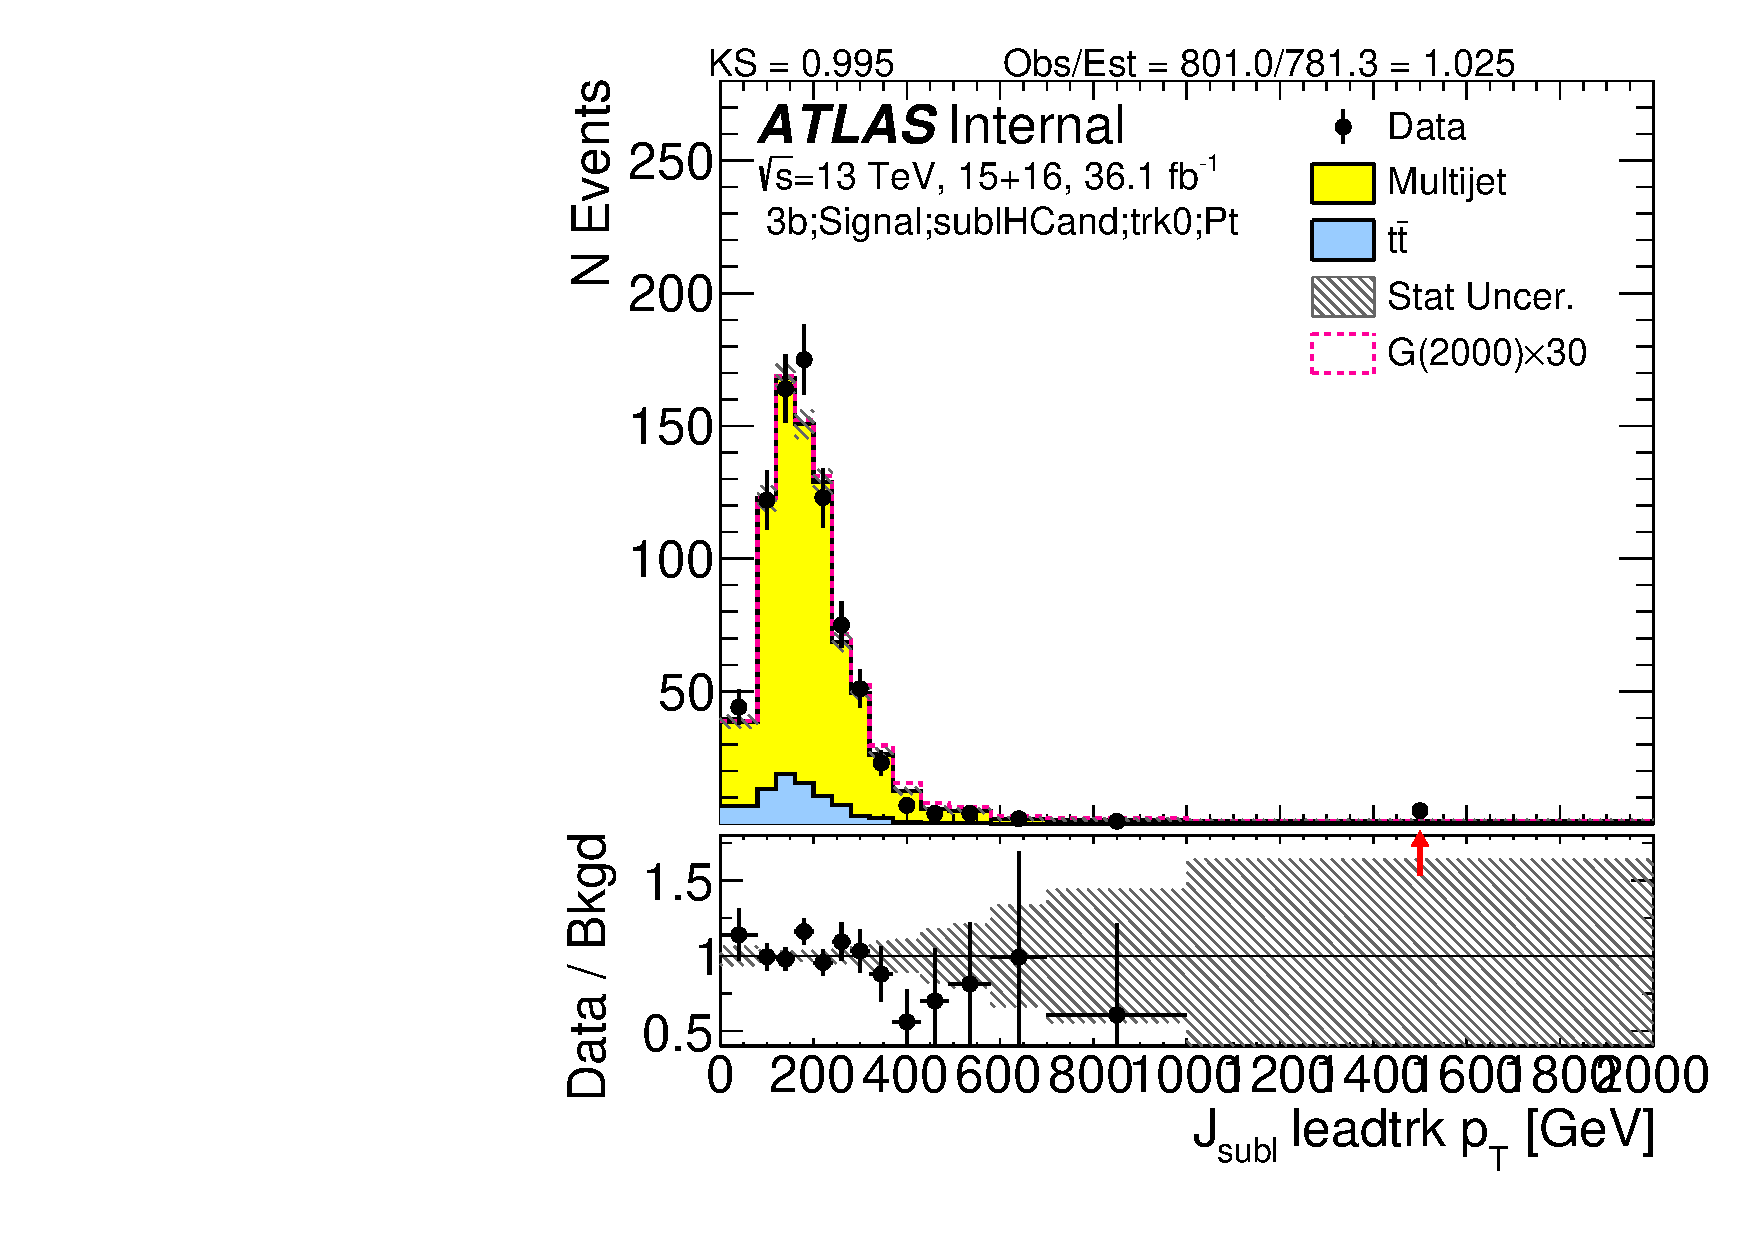
\includegraphics[angle=270, width=0.31\textwidth]{./figures/boosted/Signal/b77_ThreeTag_Signal_sublHCand_trk0_Pt.pdf}
%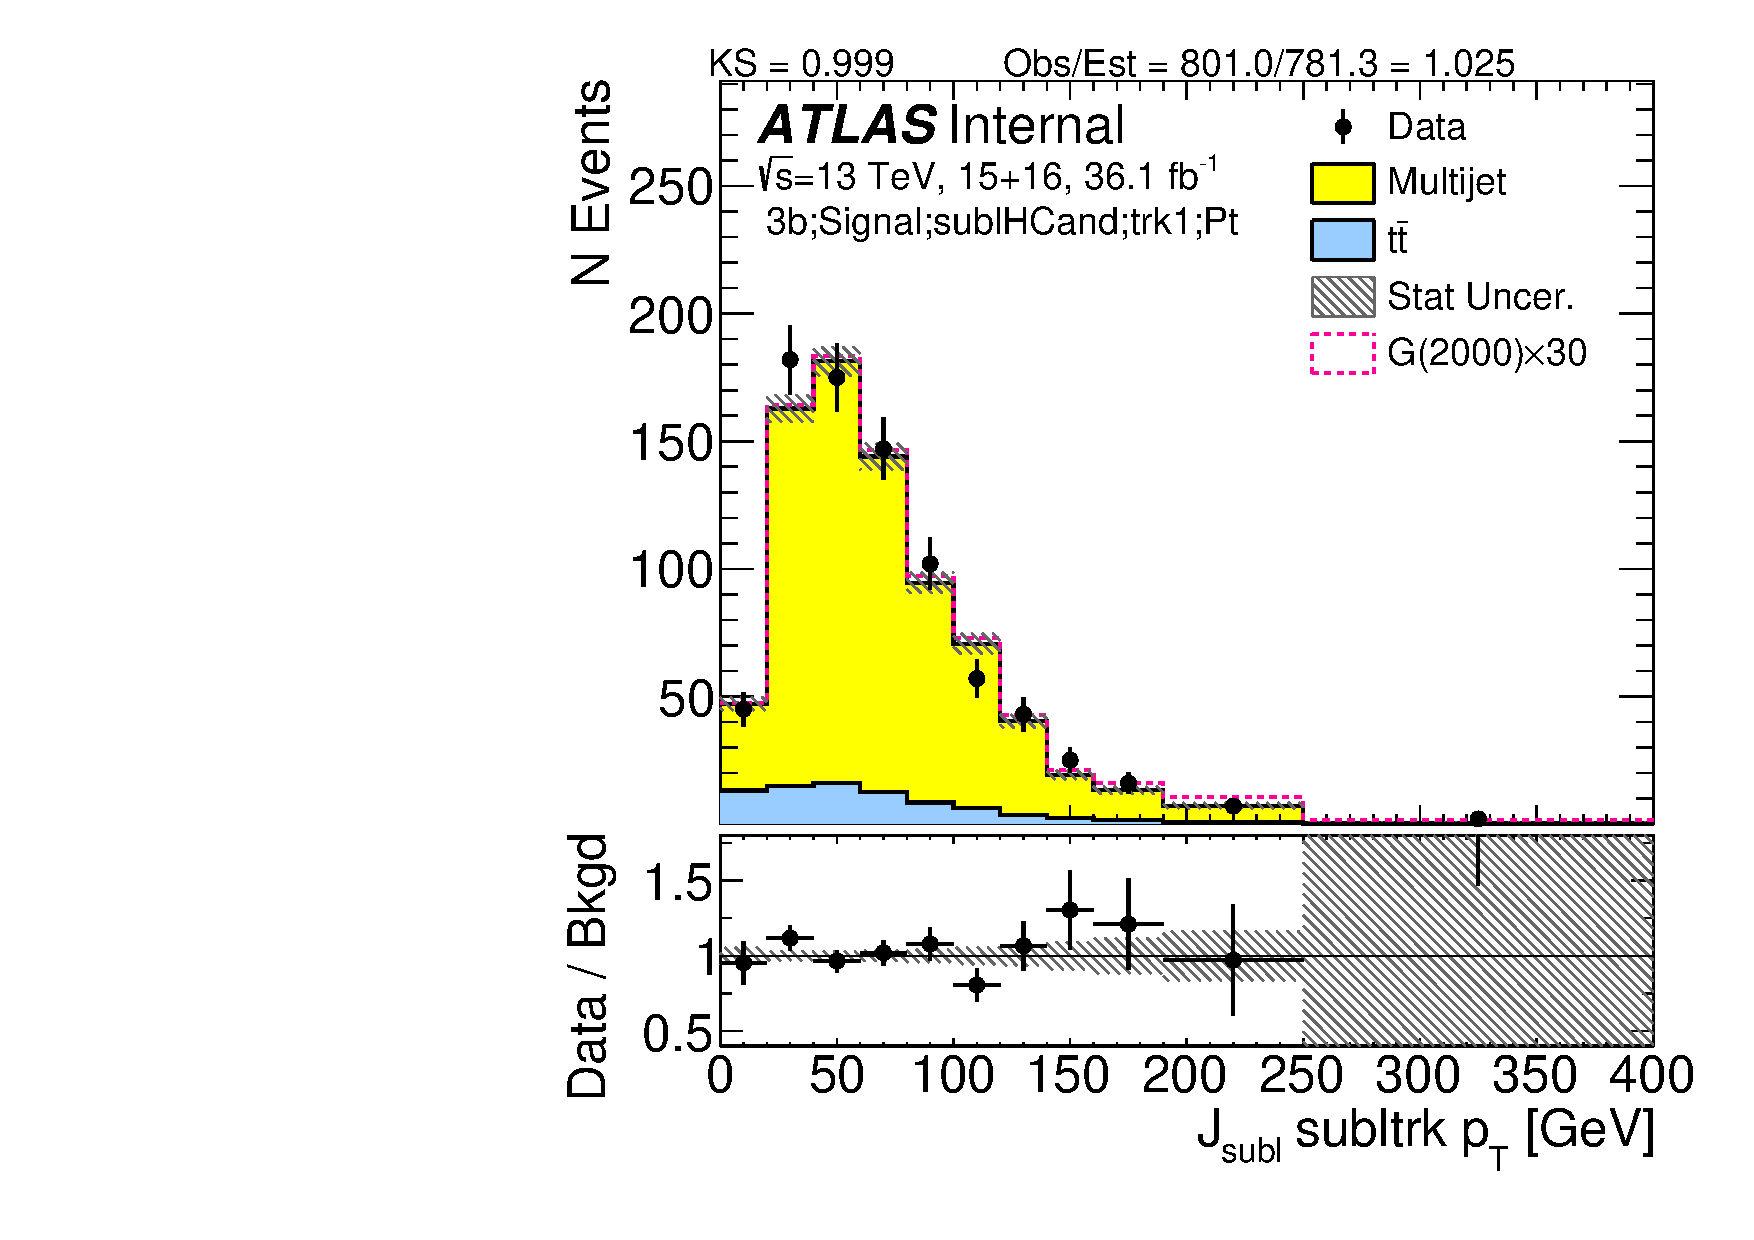
\includegraphics[angle=270, width=0.31\textwidth]{./figures/boosted/Signal/b77_ThreeTag_Signal_sublHCand_trk1_Pt.pdf}\\
%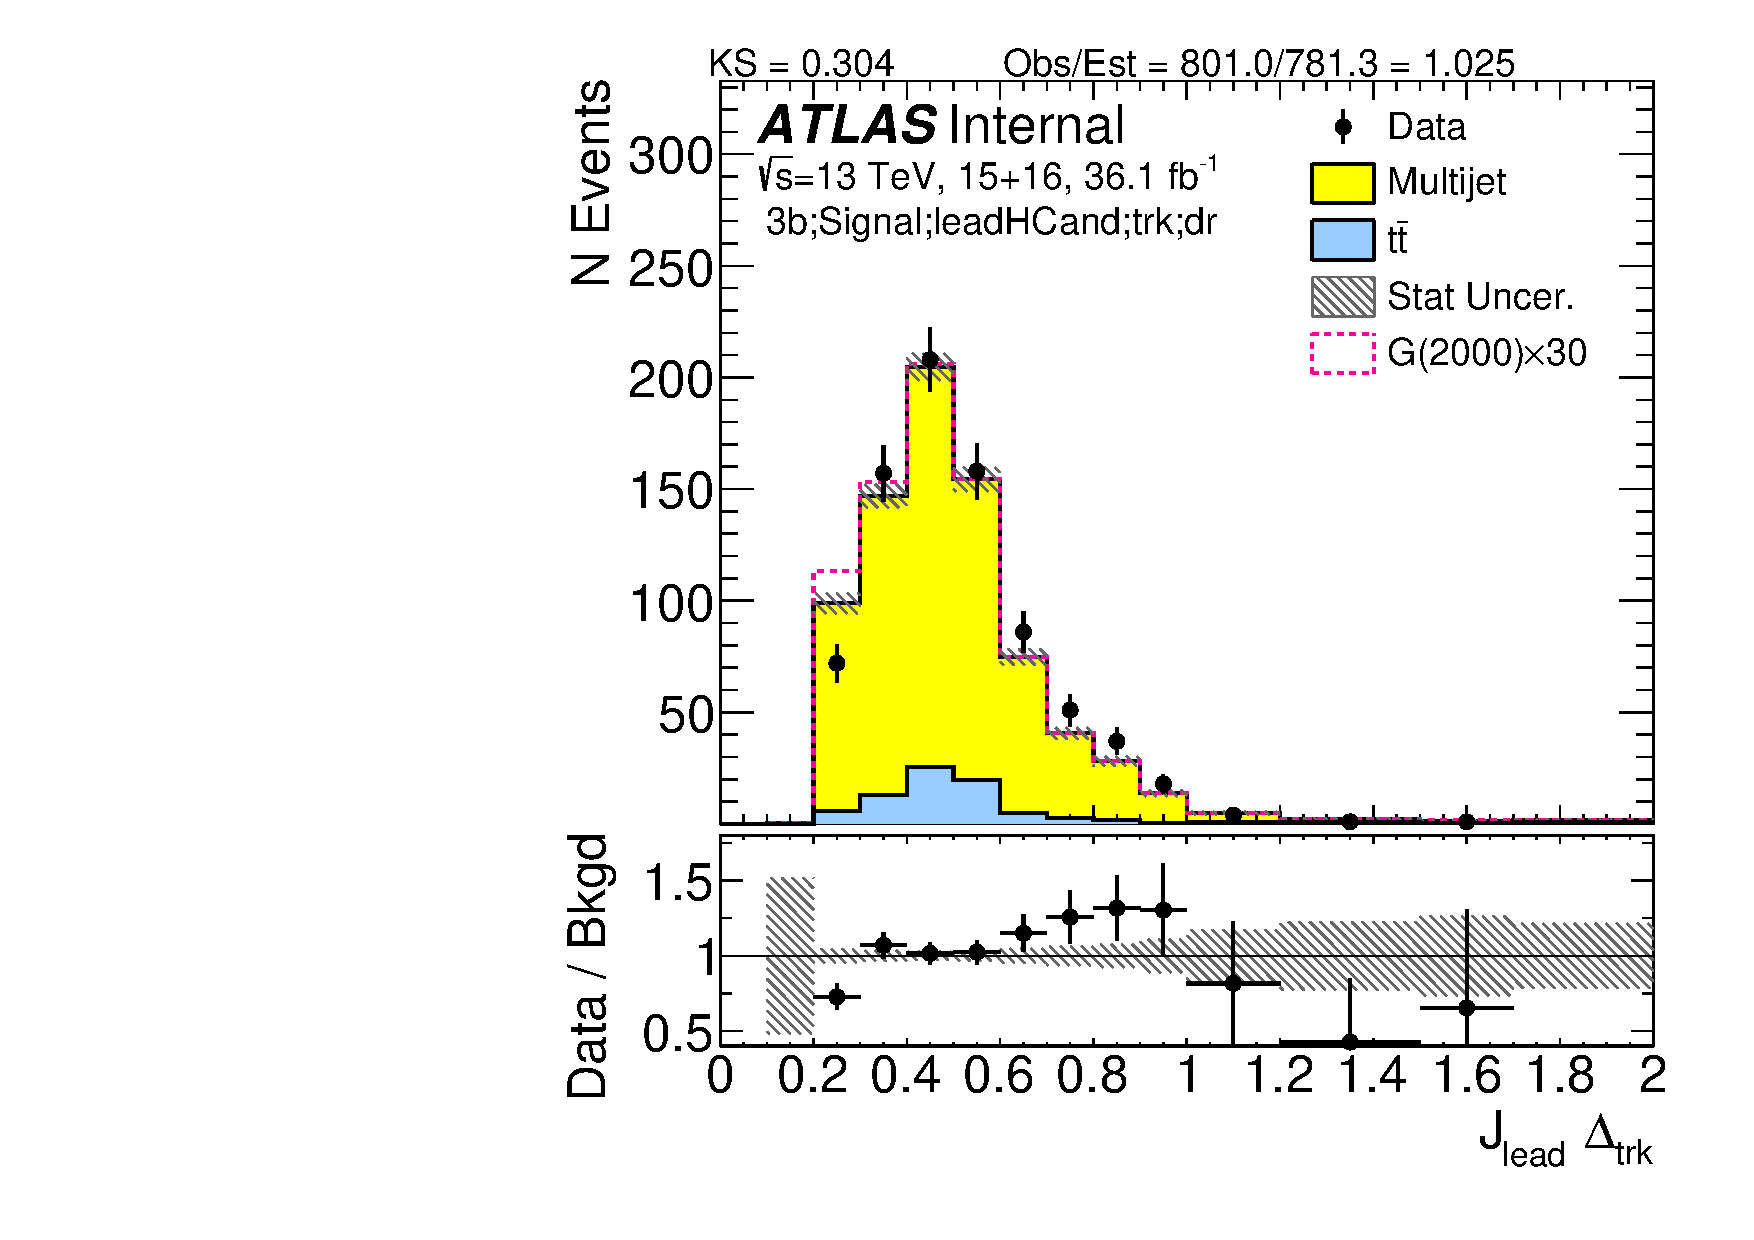
\includegraphics[angle=270, width=0.31\textwidth]{./figures/boosted/Signal/b77_ThreeTag_Signal_leadHCand_trk_dr.pdf}
%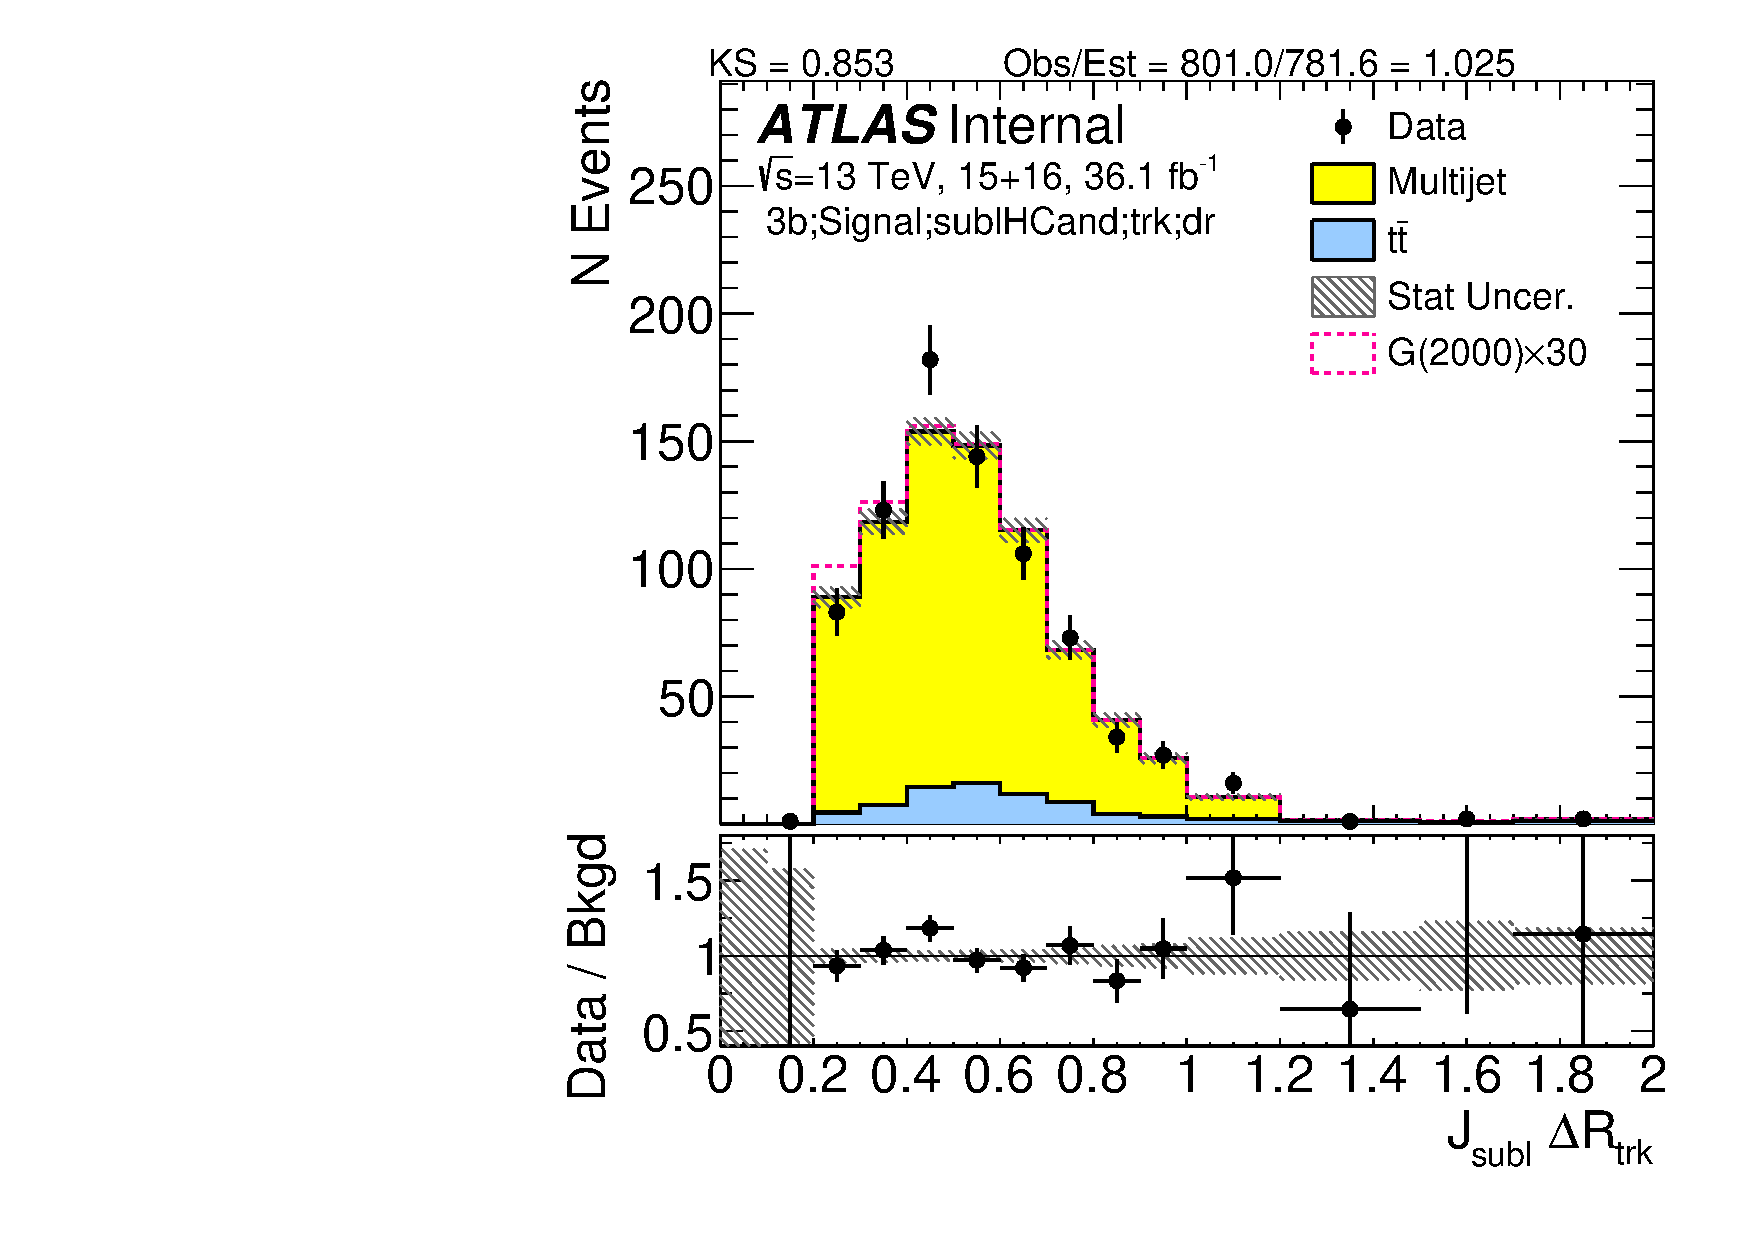
\includegraphics[angle=270, width=0.31\textwidth]{./figures/boosted/Signal/b77_ThreeTag_Signal_sublHCand_trk_dr.pdf}
  \caption{First two rows show the kinematics of the lead (left) and sub-lead (right) small-$R$ track jets associated to the lead (first-row) and sub-lead (second-row) large-$R$ jet in data and prediction in the signal region after requiring 3 $b$-tags. Third row shows the $\Delta R$ between two leading small-$R$ track-jets associated to the leading (left) and sub-leading (right) large-$R$ jet.  }
  \label{fig:boosted-3b-signal-ak2}
\end{center}
\end{figure*}


\begin{figure*}[htbp!]
\begin{center}
%\includegraphics[angle=270, width=0.31\textwidth]{./figures/boosted/Signal/b77_ThreeTag_Signal_mHH_l.pdf}
%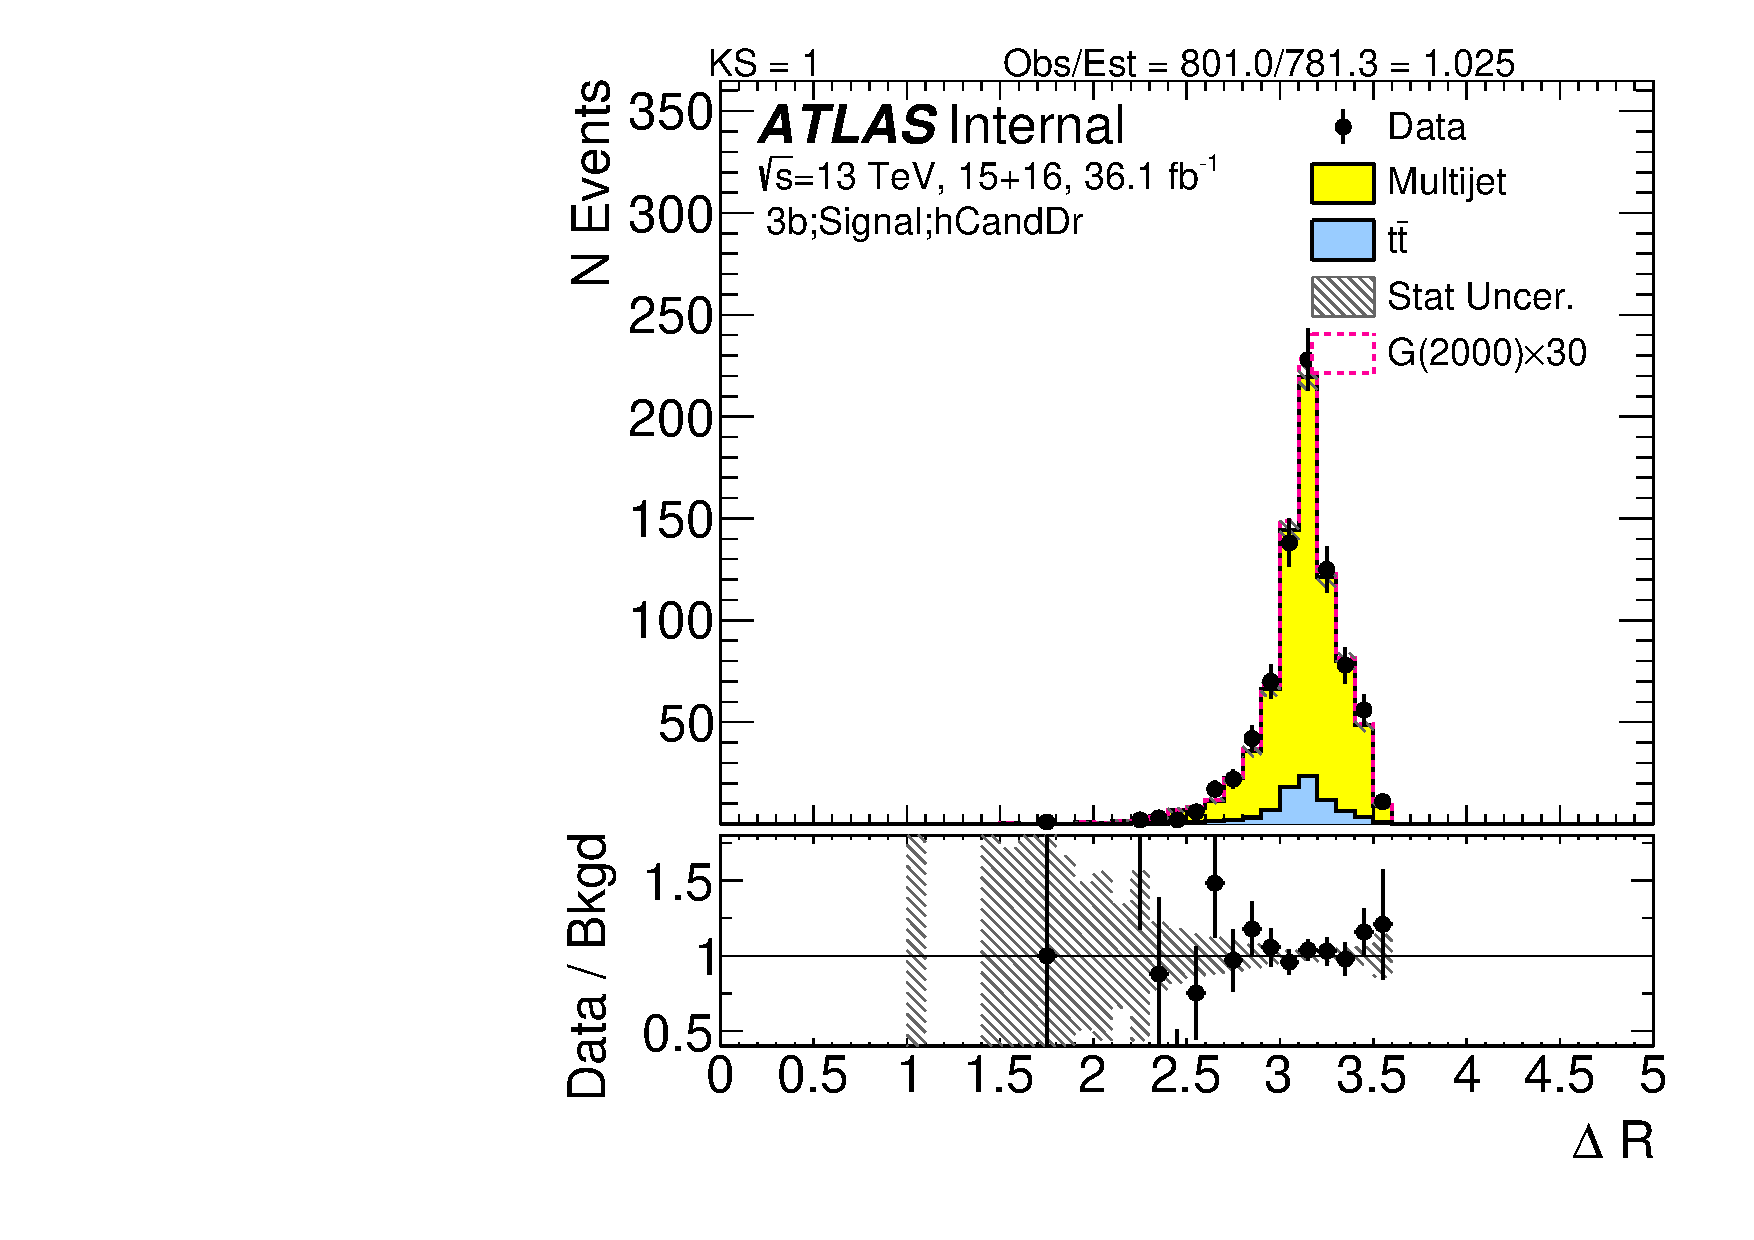
\includegraphics[angle=270, width=0.31\textwidth]{./figures/boosted/Signal/b77_ThreeTag_Signal_hCandDr.pdf}\\
%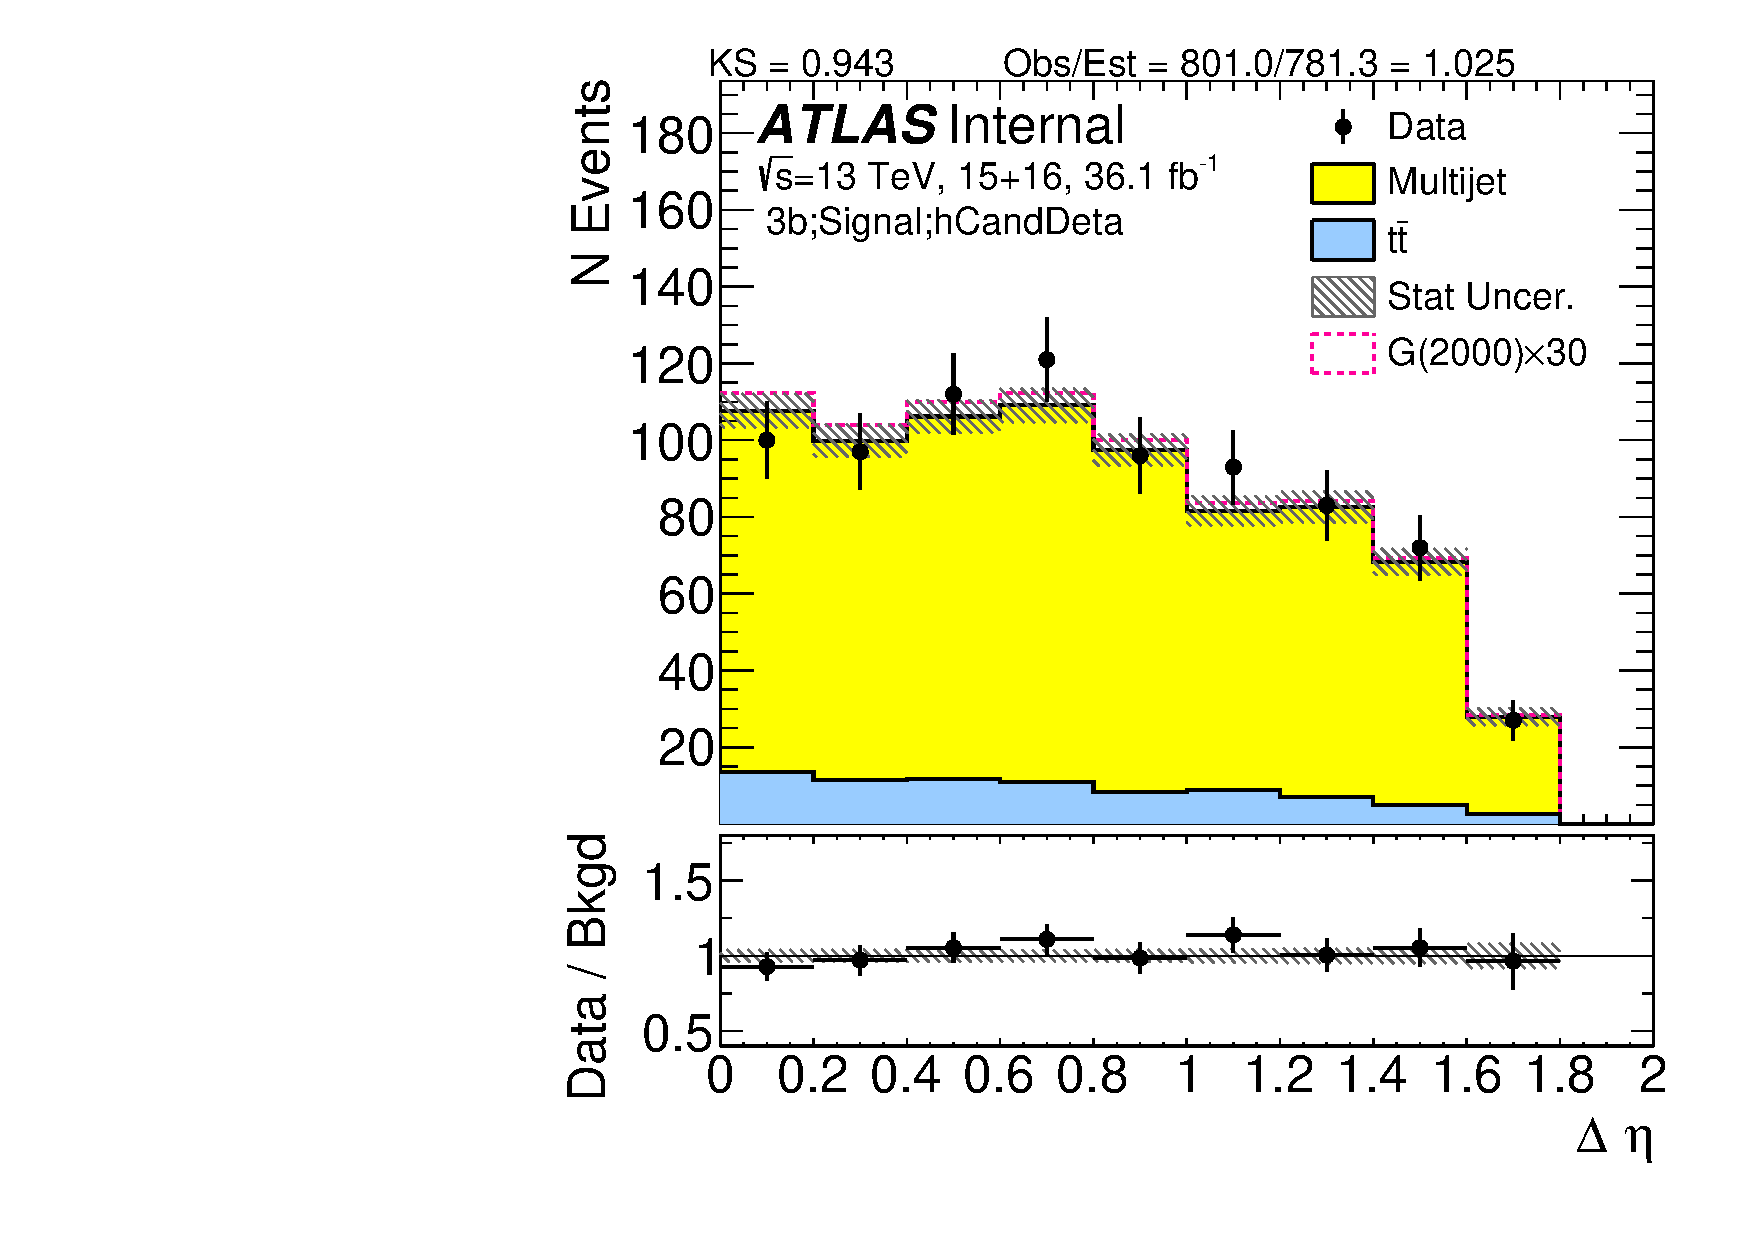
\includegraphics[angle=270, width=0.31\textwidth]{./figures/boosted/Signal/b77_ThreeTag_Signal_hCandDeta.pdf}
%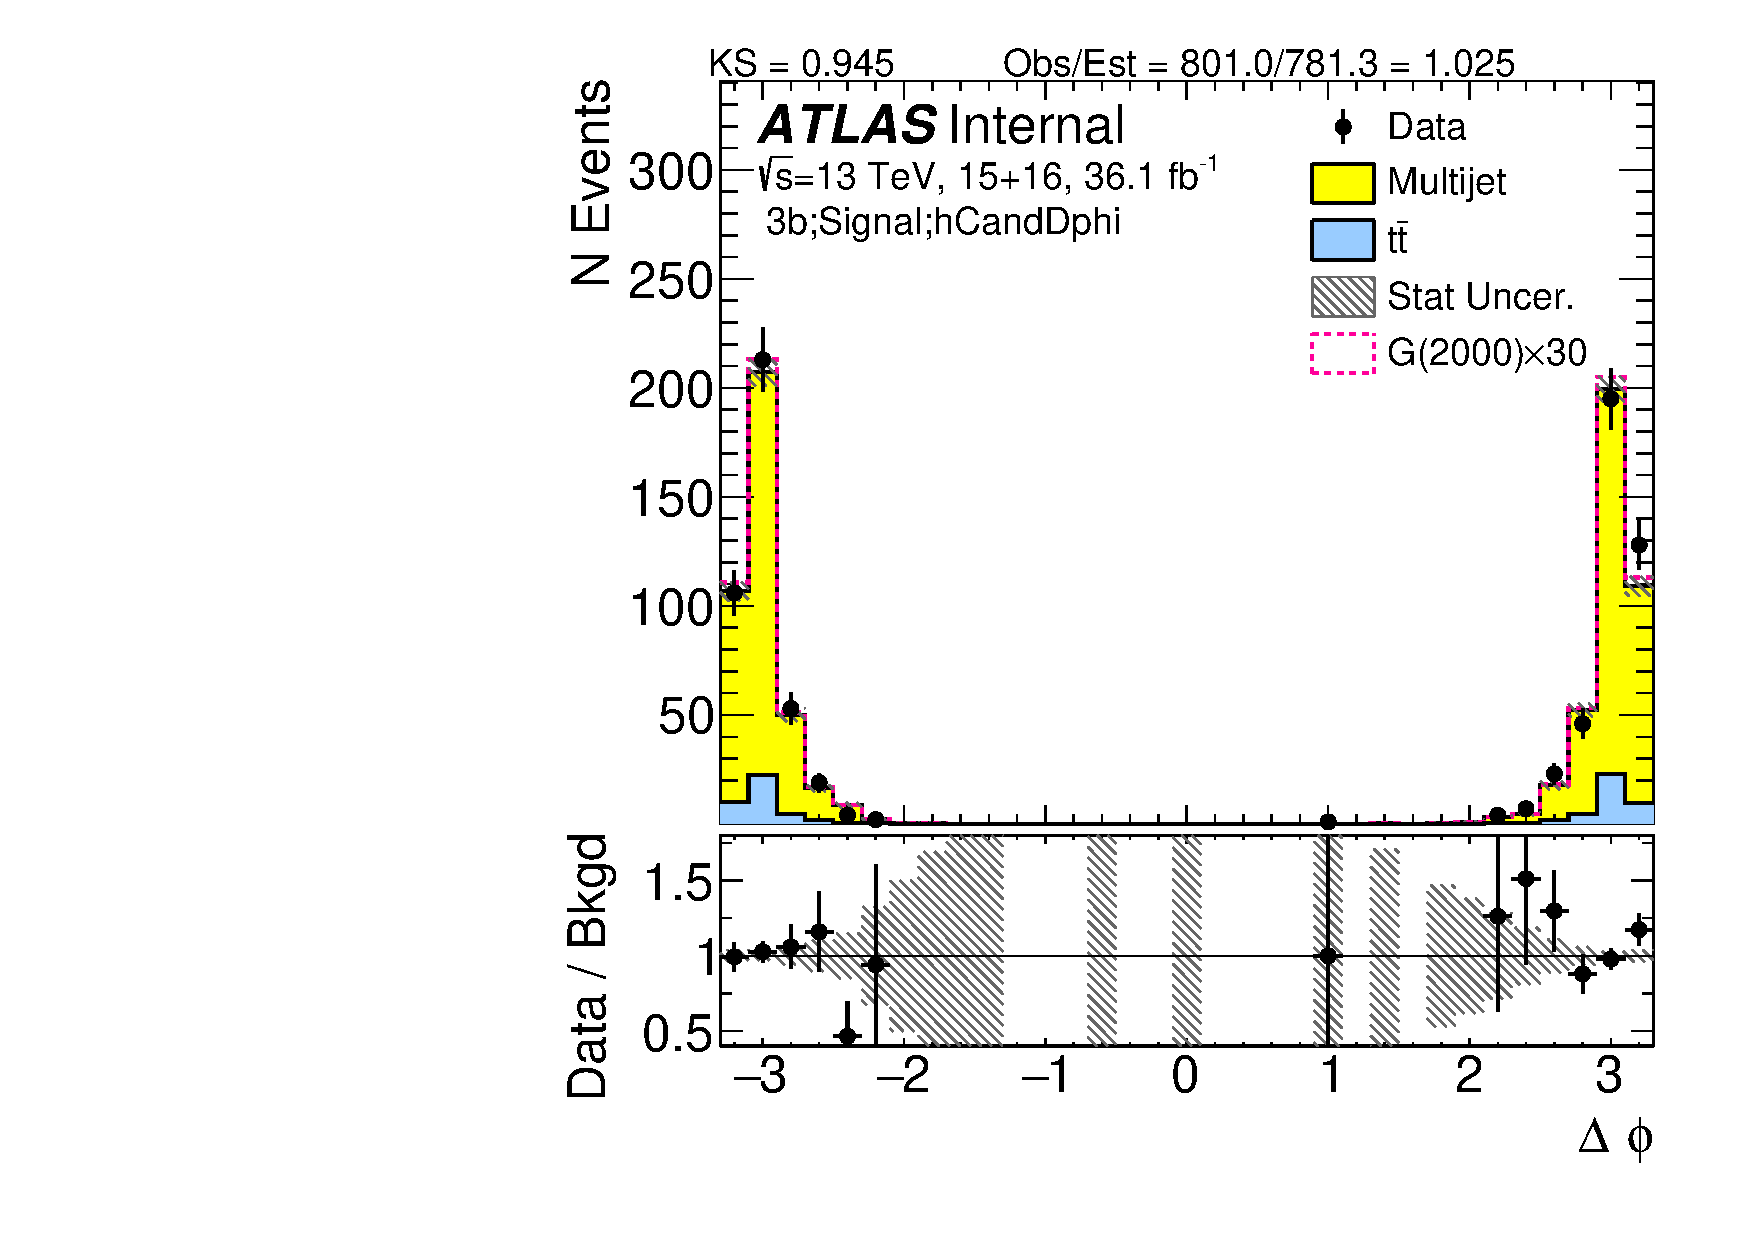
\includegraphics[angle=270, width=0.31\textwidth]{./figures/boosted/Signal/b77_ThreeTag_Signal_hCandDphi.pdf}
  \caption{Kinematics of the large-$R$ jet system in data and prediction in the signal region after requiring 3 $b$-tags.  }
  \label{fig:boosted-3b-signal-ak10-system}
\end{center}
\end{figure*}

\clearpage

\begin{figure*}[htbp!]
\begin{center}
%\includegraphics[angle=270, width=0.31\textwidth]{./figures/boosted/Signal/b77_TwoTag_split_Signal_leadHCand_Pt_m_1.pdf}
%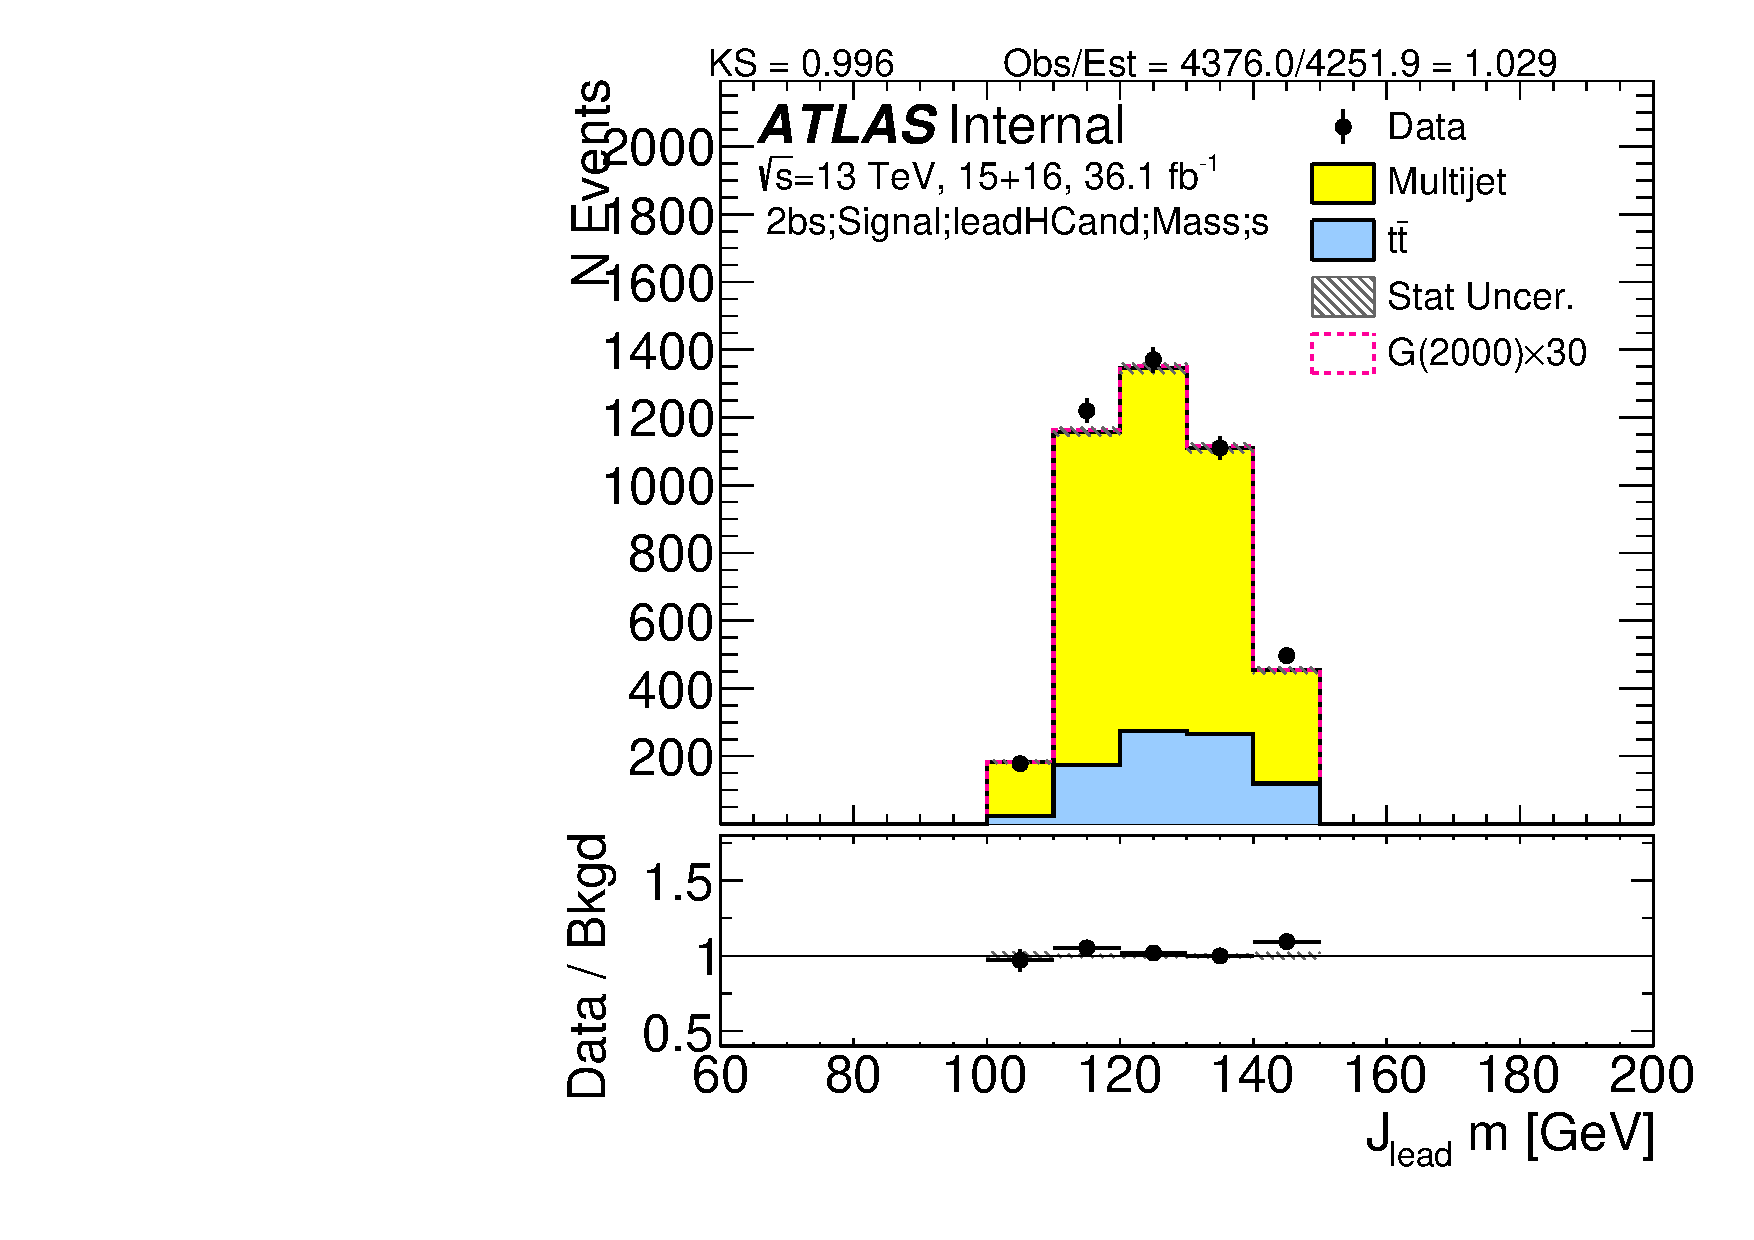
\includegraphics[angle=270, width=0.31\textwidth]{./figures/boosted/Signal/b77_TwoTag_split_Signal_leadHCand_Mass_s.pdf}\\
%\includegraphics[angle=270, width=0.31\textwidth]{./figures/boosted/Signal/b77_TwoTag_split_Signal_leadHCand_Eta.pdf}
%\includegraphics[angle=270, width=0.31\textwidth]{./figures/boosted/Signal/b77_TwoTag_split_Signal_leadHCand_Phi.pdf}
  \caption{Kinematics of the lead large-$R$ jet in data and prediction in the signal region after requiring 2 $b$-tags split. }
  \label{fig:boosted-2bs-signal-ak10-lead}
\end{center}
\end{figure*}

\begin{figure*}[htbp!]
\begin{center}
%\includegraphics[angle=270, width=0.31\textwidth]{./figures/boosted/Signal/b77_TwoTag_split_Signal_sublHCand_Pt_m_1.pdf}
%\includegraphics[angle=270, width=0.31\textwidth]{./figures/boosted/Signal/b77_TwoTag_split_Signal_sublHCand_Mass_s.pdf}\\
%\includegraphics[angle=270, width=0.31\textwidth]{./figures/boosted/Signal/b77_TwoTag_split_Signal_sublHCand_Eta.pdf}
%\includegraphics[angle=270, width=0.31\textwidth]{./figures/boosted/Signal/b77_TwoTag_split_Signal_sublHCand_Phi.pdf}
  \caption{Kinematics of the sub-lead large-$R$ jet in data and prediction in the signal region after requiring 2 $b$-tags split. }
  \label{fig:boosted-2bs-signal-ak10-subl}
\end{center}
\end{figure*}

\begin{figure*}[htbp!]
\begin{center}
%\includegraphics[angle=270, width=0.31\textwidth]{./figures/boosted/Signal/b77_TwoTag_split_Signal_leadHCand_trk0_Pt.pdf}
%\includegraphics[angle=270, width=0.31\textwidth]{./figures/boosted/Signal/b77_TwoTag_split_Signal_leadHCand_trk1_Pt.pdf}\\
%\includegraphics[angle=270, width=0.31\textwidth]{./figures/boosted/Signal/b77_TwoTag_split_Signal_sublHCand_trk0_Pt.pdf}
%\includegraphics[angle=270, width=0.31\textwidth]{./figures/boosted/Signal/b77_TwoTag_split_Signal_sublHCand_trk1_Pt.pdf}\\
%\includegraphics[angle=270, width=0.31\textwidth]{./figures/boosted/Signal/b77_TwoTag_split_Signal_leadHCand_trk_dr.pdf}
%\includegraphics[angle=270, width=0.31\textwidth]{./figures/boosted/Signal/b77_TwoTag_split_Signal_sublHCand_trk_dr.pdf}
  \caption{First two rows show the kinematics of the lead (left) and sub-lead (right) small-$R$ track jets associated to the lead (first-row) and sub-lead (second-row) large-$R$ jet in data and prediction in the signal region after requiring 2 $b$-tags split. Third row shows the $\Delta R$ between two leading small-$R$ track-jets associated to the leading (left) and sub-leading (right) large-$R$ jet.  }
  \label{fig:boosted-2bs-signal-ak2}
\end{center}
\end{figure*}


\begin{figure*}[htbp!]
\begin{center}
%\includegraphics[angle=270, width=0.31\textwidth]{./figures/boosted/Signal/b77_TwoTag_split_Signal_mHH_l_1.pdf}
%\includegraphics[angle=270, width=0.31\textwidth]{./figures/boosted/Signal/b77_TwoTag_split_Signal_hCandDr.pdf}\\
%\includegraphics[angle=270, width=0.31\textwidth]{./figures/boosted/Signal/b77_TwoTag_split_Signal_hCandDeta.pdf}
%\includegraphics[angle=270, width=0.31\textwidth]{./figures/boosted/Signal/b77_TwoTag_split_Signal_hCandDphi.pdf}
  \caption{Kinematics of the large-$R$ jet system in data and prediction in the signal region after requiring 2 $b$-tags split.  }
  \label{fig:boosted-2bs-signal-ak10-system}
\end{center}
\end{figure*}

\clearpage
\subsection{Test of the background model hypothesis}
A search for statistically significant deviation from the background model hypothesis is
performed following the procedure described in Sec.\,\ref{sec-search-procedure}, computing the
local $p_0$ value using the asymptotic approximation.

The background model is found to describe the data and no significative excess is observed, with $p_0$ as a function of \mGrav shown in Figure~\ref{fig:p0_RSG10}. The largest discrepancy observed, at $\mGrav=1.5\,\GeV$, has a local significance of only 1.1 $\sigma$.

\begin{figure}[ht!]
\begin{center}
 %\includegraphics[angle=270, width=0.48\textwidth]{figures/boosted/Limit_FullSyst/p0_hh.pdf}
\caption{Local $p_0$ value for the boosted analysis, analysed as a function of the Graviton mass for the KK graviton model
with $c \equiv k/\bar{M}_P = 1.0$.}
\label{fig:p0_RSG10}
\end{center}
\end{figure}

\subsection{Observed Limits}
\label{sec:observedlimits}

The observed exclusion limits for the KK graviton model with  $c \equiv k/\bar{M}_P = 1.0$
and including only statistical uncertainty are shown in Figure ~\ref{fig:brazil_hh_boosted_4b_c10_stat_unblinded}, ~\ref{fig:brazil_hh_boosted_3b_c10_stat_unblinded}, ~\ref{fig:brazil_hh_boosted_2b_c10_stat_unblinded}. The combined limit of the three channels is shown in Figure ~\ref{fig:brazil_hh_boosted_all_c10_stat_unblinded}. 

\begin{figure*}
\begin{center}
%\includegraphics[angle=270, width=0.75\textwidth]{figures/boosted/Limit_Stat/BrazilPlot_asymptotics_hh_boosted_4b_unblinded_c10.pdf}
\caption{The expected and observed 95\% C.L. exclusion limits for the boosted $4b$ analysis calculated including statistical uncertainty only
for the KK graviton model with $c \equiv k/\bar{M}_P = 1.0$. Limits are derived within the asymptotic approximation.}
\label{fig:brazil_hh_boosted_4b_c10_stat_unblinded}
\end{center}
\end{figure*}

\begin{figure*}
\begin{center}
%\includegraphics[angle=270, width=0.75\textwidth]{figures/boosted/Limit_Stat/BrazilPlot_asymptotics_hh_boosted_3b_unblinded_c10.pdf}
\caption{The expected and observed 95\% C.L. exclusion limits for the boosted $3b$ analysis calculated including statistical uncertainty only
for the KK graviton model with $c \equiv k/\bar{M}_P = 1.0$. Limits are derived within the asymptotic approximation.}
\label{fig:brazil_hh_boosted_3b_c10_stat_unblinded}
\end{center}
\end{figure*}

\begin{figure*}
\begin{center}
%\includegraphics[angle=270, width=0.75\textwidth]{figures/boosted/Limit_Stat/BrazilPlot_asymptotics_hh_boosted_2b_unblinded_c10.pdf}
\caption{The expected and observed 95\% C.L. exclusion limits for the boosted $2bs$ analysis calculated including statistical uncertainty only
for the KK graviton model with $c \equiv k/\bar{M}_P = 1.0$. Limits are derived within the asymptotic approximation.}
\label{fig:brazil_hh_boosted_2b_c10_stat_unblinded}
\end{center}
\end{figure*}


\begin{figure*}
\begin{center}
%\includegraphics[angle=270, width=0.75\textwidth]{figures/boosted/Limit_Stat/BrazilPlot_asymptotics_hh_boosted_all_unblinded_c10.pdf}
\caption{The expected and observed 95\% C.L. exclusion limits for the combined boosted analysis calculated including statistical uncertainty only
for the KK graviton model with $c \equiv k/\bar{M}_P = 1.0$. Limits are derived within the asymptotic approximation. }
\label{fig:brazil_hh_boosted_all_c10_stat_unblinded}
\end{center}
\end{figure*}

Figure \ref{fig:fullSystLimit_c10_combined} shows the 95\% C.L. cross-section exclusion limits for the bulk RS model with \kMPl = 1, including full systematic uncertainties. Examples of the fit used to set these limits are shown in Figure \ref{fig:postFitSRs}, in this case considering a bulk RS gravition signal with  $\mGrav = 1.3\,\TeV$ and $\kMPl = 1$. Good agreement is seen between data and the background model, but an insignificant signal contribution is fitted at $\mGrav = 1.3\,\TeV$. This fluctuation is why the observed limit is higher than the expected at this mass in Figure \ref{fig:fullSystLimit_c10_combined}.

\begin{figure*}
\begin{center}
%\includegraphics[angle=270, width=0.75\textwidth]{figures/boosted/Limit_FullSyst/BrazilPlot_Asymptotic_RSGC10_merged_FullSyst_unblinded.pdf}
\caption{The expected and observed 95\% C.L. exclusion limits for the combined boosted analysis calculated including all sources of uncertainty,
for the bulk RS model with $c \equiv k/\bar{M}_P = 1.0$. Limits are derived within the asymptotic approximation.}
\label{fig:fullSystLimit_c10_combined}
\end{center}
\end{figure*}

\begin{figure*}[htbp!]
\begin{center}
%\subfloat[2-Tag Signal Region]{%\includegraphics[angle=270, width=0.5\textwidth]{./figures/boosted/Limit_FullSyst/2bPostFit.pdf}%\includegraphics[angle=270, width=0.5\textwidth]{./figures/boosted/Limit_FullSyst/2bPostFit_Log.pdf}}\\
%\subfloat[3-Tag Signal Region]{%\includegraphics[angle=270, width=0.5\textwidth]{./figures/boosted/Limit_FullSyst/3bPostFit.pdf}%\includegraphics[angle=270, width=0.5\textwidth]{./figures/boosted/Limit_FullSyst/3bPostFit_Log.pdf}}\\
%\subfloat[4-Tag SignalRegion]{%\includegraphics[angle=270, width=0.5\textwidth]{./figures/boosted/Limit_FullSyst/4bPostFit.pdf}%\includegraphics[angle=270, width=0.5\textwidth]{./figures/boosted/Limit_FullSyst/4bPostFit_Log.pdf}}\\
  \caption{Total background predictions before and after the conditional likelihood fit compared to data, for: (a) the 2-tag-split signal region; (b) the 3-tag signal region; and (c) the 4-tag signal region. In this case, a bulk RS graviton signal with $\mGrav=1.3\,\TeV$ and $\kMPl=1.0$ is considered. Good agreement is also observed in all signal regions with a fixed $\mu=0$.}
  \label{fig:postFitSRs}
\end{center}
\end{figure*}

Figure \ref{fig:nuisanceParams}, \ref{fig:nuisanceParams2} shows the pull of the systematic uncertainty nuisance parameters and their correlations. One nuisance parameter in both the $2b$ and $3b$ samples shows a significant constraint coming from the signal region data. This nuisance parameter corresponds to the shape uncertainty on the QCD background derived from the $2b$ and $3b$ control regions, as explained in Section \ref{unc-shape-qcd-in-sr}. The prior probability distributions for this nuisance parameter is very broad, with the relative uncertainty on the background prediction reaching 15000\% at high $m_{hh}$. This is because there is very little data in the control region at high mass to constrain the uncertainty. In the signal region however, the two events found suffice to constrain it: very tightly in comparison to the extremely loose prior constraint.

\begin{figure*}[htbp!]
\begin{center}
%\subfloat[2-Tag Split Background Uncertainties]{%\includegraphics[angle=270, width=0.75\textwidth]{./figures/boosted/Limit_FullSyst/NuisanceParam_2b.pdf}}\\
%\subfloat[3-Tag Background Uncertainties]{%\includegraphics[angle=270, width=0.75\textwidth]{./figures/boosted/Limit_FullSyst/NuisanceParam_3b.pdf}}\\
%\subfloat[4-Tag Background Uncertainties]{%\includegraphics[angle=270, width=0.75\textwidth]{./figures/boosted/Limit_FullSyst/NuisanceParam_4b.pdf}}\\
  \caption{Nuisance parameters associated with the background modelling, after the conditional likelihood fit for a bulk RS graviton signal with $\mGrav=1.5\,\TeV$ and $\kMPl=1.0$. The tight constraints of 2b\_QCD\_CRShape and 3b\_QCD\_CRShape are a result of the nuisance parameter prior being unconstrained due to a lack of control region data at high mass.}
  \label{fig:nuisanceParams}
\end{center}
\end{figure*}

\begin{figure*}[htbp!]
\begin{center}
%\subfloat[B-tagging uncertainties]{%\includegraphics[angle=270, width=0.75\textwidth]{./figures/boosted/Limit_FullSyst/NuisanceParam_BTag.pdf}}\\
%\subfloat[Other uncertainties]{%\includegraphics[angle=270, width=0.75\textwidth]{./figures/boosted/Limit_FullSyst/NuisanceParam_Others.pdf}}
\caption{Nuisance parameters associated with the detector simulation and theoretical modelling of the signal and \ttbar, after the conditional likelihood fit for a bulk RS graviton signal with $\mGrav=1.5\,\TeV$ and $\kMPl=1.0$. The tight constraints of 2b\_QCD\_CRShape and 3b\_QCD\_CRShape are a result of the nuisance parameter prior being unconstrained due to a lack of control region data at high mass.}
  \label{fig:nuisanceParams2}
\end{center}
\end{figure*}  
